\documentclass{report}

\usepackage[T1]{fontenc}
\usepackage[utf8]{inputenc}
\usepackage{times}

\usepackage[font=small,labelfont=bf,tableposition=top]{caption}
\usepackage{graphicx}
\usepackage{natbib} 

\usepackage{amsmath}
\usepackage{amsfonts}
\usepackage{amssymb}
\usepackage{color, soul}
\usepackage{hyperref}
\usepackage{algorithmicx}
\usepackage{algpseudocode}
\usepackage{subfigure}
\usepackage{stmaryrd}

\renewcommand{\vec}[1]{\boldsymbol{{#1}}} 
\newcommand{\duesoon}[1]{{\sethlcolor{green}\hl{#1}}}
\usepackage{mathrsfs}


\newtheorem{theorem}{Theorem}
\newtheorem{acknowledgement}[theorem]{Acknowledgement}
\newtheorem{algorithm}[theorem]{Algorithm}
\newtheorem{axiom}[theorem]{Axiom}
\newtheorem{case}[theorem]{Case}
\newtheorem{claim}[theorem]{Claim}
\newtheorem{conclusion}[theorem]{Conclusion}
\newtheorem{condition}[theorem]{Condition}
\newtheorem{conjecture}[theorem]{Conjecture}
\newtheorem{corollary}[theorem]{Corollary}
\newtheorem{criterion}[theorem]{Criterion}
\newtheorem{definition}[theorem]{Definition}
\newtheorem{example}[theorem]{Example}
\newtheorem{exercise}[theorem]{Exercise}
\newtheorem{lemma}[theorem]{Lemma}
\newtheorem{notation}[theorem]{Notation}
\newtheorem{problem}[theorem]{Problem}
\newtheorem{proposition}[theorem]{Proposition}
\newtheorem{remark}[theorem]{Remark}
\newtheorem{solution}[theorem]{Solution}
\newtheorem{summary}[theorem]{Summary}
\newenvironment{proof}[1][Proof]{\textbf{#1.} }{\ \rule{0.5em}{0.5em}}

\newtheorem{guess}{Definition}
\newcommand{\comment}[1] {}
\newcommand{\Norder} {N}
\newcommand{\order}{\mathcal{O}}
\newcommand{\Npoints} {N_p}
\newcommand{\Nfaces} {N_{f}}
\newcommand{\Nelements} {N_e}

\newcommand{\eps}{\varepsilon}
\newcommand{\Dweak}{\wt{D}}
\newcommand{\diff}[2] {\frac{\partial #1}{\partial #2}}
\newcommand{\dxx}[2] {\frac{\partial^2 #1}{\partial {#2}^2}}
\newcommand{\difft}[2] {\frac{d #1}{d #2}}
\newcommand{\dxxt}[2] {\frac{d^2 #1}{d {#2}^2}}
\newcommand{\lagrange}[1] {\frac{d #1}{dt}}
\newcommand{\lebesgue}{\parallel I \parallel}
\newcommand{\polysp}{\mathcal{P}_N}
\newcommand{\laplacian}{\nabla^2}
\newcommand{\divergence}{\nabla \cdot}
\newcommand{\inte}{\int_{\mbox{\footnotesize ${\Omega_e}$}}}
\newcommand{\intb}{\int_{\mbox{\footnotesize ${\Gamma_e}$}}}
\newcommand{\intce}{\int_{\mbox{\footnotesize ${\widehat{\Omega}_e}$}}}
\newcommand{\intcb}{\int_{\mbox{\footnotesize ${\widehat{\Gamma}_e}$}}}
\newcommand{\intg}{\int_{\mbox{\footnotesize ${\Omega}$}}}
\newcommand{\intgb}{\int_{\mbox{\footnotesize ${\Gamma}$}}}
\newcommand{\intv}{\int_{\mbox{\footnotesize ${\sigma}$}}}
\newcommand{\sumv}{\sum_{K=1}^{N_{\mathrm{lev}}}}
\newcommand{\sumk}{\sum_{L=1}^{K}}
\newcommand{\sumN}{\sum_{i=1}^{N+1}}
\newcommand{\half}{\frac{1}{2}}
\newcommand{\inti}{\int_{\mbox{\footnotesize\sf I}}}
\newcommand{\intbd}{\oint_{\mbox{\footnotesize ${\delta}$\sf D}}}
\newcommand{\intbi}{\oint_{\mbox{\footnotesize ${\delta}$\sf I}}}
\newcommand{\ldnorm}[1]{\left\| #1 \right\|_{\mbox{\footnotesize \sf D}} }
\newcommand{\lonorm}[1]{\left\| #1 \right\|_{\Omega}}
\newcommand{\spc}[1]{\mbox{\sf #1}}
\newcommand{\ope}[1]{{\cal #1}}
\newcommand{\mt}[1]{{\rm #1}}
\newcommand{\dis}{\displaystyle}
\newcommand{\ve}{\varepsilon}
\newcommand{\ov}{\overline}
\newcommand{\wt}{\widetilde}
\newcommand{\wh}{\widehat}
\newcommand{\Dhat}{\widehat{D}}
\newcommand{\be}{\begin{equation}}
\newcommand{\ee}{\end{equation}}
\newcommand{\bea}{\begin{eqnarray*}}
\newcommand{\eea}{\end{eqnarray*}}
\newcommand{\Jace}{J^{(e)}}
\newcommand{\Jacl}{J^{(l)}}
\def\bepsilon{\mbox{\boldmath $\epsilon $}}
\def\bpsi{\mbox{\boldmath $\psi $}}
\def\bphi{\mbox{\boldmath $\phi $}}
\def\bmu{\mbox{\boldmath $\mu $}}
\def\Et{ \tilde{E} }
\def\Ht{ \tilde{H} }
\def\sdot{ \dot{\sigma} }

\newcommand{\fstar}{f^{(*)}}

\DeclareMathOperator{\Span}{span}
\DeclareMathOperator{\Dim}{dim}

\newcommand{\polyquad}{\mathcal{Q}_{N}}
\newcommand{\polyP}{\mathcal{P}_{N}}
\newcommand{\polyPnpm}{\mathcal{P}_{(N+M)}}
\newcommand{\polyPd}{\mathcal{P}_{d}}
\newcommand{\polyPnm}{\mathcal{P}_{N,M}}
\newcommand{\polyPn}{\mathcal{P}_{N,0}}
\newcommand{\transpose}{^{\mathcal{T}}}

\newcommand{\vecQ}{\vec{Q}}
\newcommand{\vecQe}{\vec{Q}^{(e)}}
\newcommand{\vecFe}{\vec{\mathcal{F}}^{(e)}}
\newcommand{\statevec}{\vec{Y}}
\newcommand{\statevecN}{\vec{Y}_N^{(e)}}
\newcommand{\statestage}{\vec{\mathcal{Y}}}
\newcommand{\Ftensor}{\vec{F}(\qvector)}
\newcommand{\FtensorN}{\vec{F}\left( \qvectorN \right)}
\newcommand{\FtensorStar}{\vec{F}\left( \qvector_N^{(e,k)} \right)}
\newcommand{\Svector}{S(\qvector)}
\newcommand{\SvectorN}{S \left( \qvectorN \right)}
\newcommand{\qref}{\vec{q}_0}
\newcommand{\qvectorb}{\vec{q}_b}
\newcommand{\qtt}{\vec{q}_{tt}}
\newcommand{\qhat}{\widehat{\vec{q}}}
\newcommand{\qhatb}{\widehat{\vec{q}}_b}
\newcommand{\qelem}{q^{(e)}}
\newcommand{\rhoref}{\rho_0}
\newcommand{\piref}{\pi_0}
\newcommand{\Thetaref}{\Theta_0}
\newcommand{\Gref}{G_0}
\newcommand{\Tref}{T_0}
\newcommand{\thetaref}{\theta_0}
\newcommand{\Pref}{{P}_0}
\newcommand{\Eref}{{E}_0}
\newcommand{\Href}{{h}_0}
\newcommand{\rhohat}{\widehat{\rho}}
\newcommand{\pihat}{\widehat{\pi}}
\newcommand{\Phat}{\widehat{P}}
\newcommand{\uvechat}{\widehat{{\mbox{\boldmath$u$\unboldmath}}}}
\newcommand{\uhathat}{\widehat{\widehat{{\mbox{\boldmath$u$\unboldmath}}}}}
\newcommand{\Uhat}{\widehat{{\mbox{\boldmath$U$\unboldmath}}}}
\newcommand{\Uhathat}{\widehat{\widehat{{\mbox{\boldmath$U$\unboldmath}}}}}
\newcommand{\thetahat}{\widehat{\theta}}
\newcommand{\Thetahat}{\widehat{\Theta}}
\newcommand{\Ehat}{\widehat{E}}
\newcommand{\uhat}{\widehat{u}}
\newcommand{\vhat}{\widehat{v}}
\newcommand{\what}{\widehat{w}}
\newcommand{\pitt}{\pi_{tt}}
\newcommand{\rhott}{\rho_{tt}}
\newcommand{\Ett}{E_{tt}}
\newcommand{\Utt}{\vec{U}_{tt}}
\newcommand{\uvectt}{\vec{u}_{tt}}
\newcommand{\utt}{u_{tt}}
\newcommand{\vtt}{v_{tt}}
\newcommand{\wtt}{w_{tt}}
\newcommand{\Ptt}{P_{tt}}
\newcommand{\vecPtt}{\vec{P}_{tt}}
\newcommand{\Thetatt}{\Theta_{tt}}
\newcommand{\thetatt}{\theta_{tt}}
%Projector Matrices
\newcommand{\projmatrix}{\vec{\mathcal{P}}}
\newcommand{\qmatrix}{\vec{\mathcal{Q}}}
\newcommand{\pcmatrix}{\vec{\mathcal{P}}_C}
\newcommand{\Cmatrix}{\left(\vec{\mathcal{C}}^{(e,f)}\right)\transpose}
\newcommand{\Dmatrix}{\vec{D}^{(e)}}
\newcommand{\Dwmatrix}{\wt{\vec{D}}^{(e)}}
\newcommand{\Mmatrix}{M^{(e)}}
\newcommand{\Fmatrix}{\vec{F}^{(e,l)}}
\newcommand{\Gmatrix}{\mathcal{G}}
\newcommand{\Umatrix}{\mathcal{U}^{(e,f)}}
\newcommand{\amatrix}{\vec{\mathcal{A}}}
\newcommand{\rmatrix}{\vec{\mathcal{R}}}
%Vectors
\newcommand{\nvector}{\wh{\vec{n}}_{\Gamma}}
\newcommand{\nhat}{\wh{\vec{n}}}
\newcommand{\ivector}{\wh{\vec{i}}}
\newcommand{\jvector}{\wh{\vec{j}}}
\newcommand{\kvector}{\wh{\vec{k}}}
\newcommand{\rvector}{\wh{\vec{r}}}
\newcommand{\svector}{\wh{\vec{s}}}
\newcommand{\tvector}{\wh{\vec{t}}}
\newcommand{\vvector}{\wh{\vec{v}}}
\newcommand{\Qvector}{\vec{Q}}
%Vectors
\newcommand{\ur}{{u}^{(r)}}
\newcommand{\us}{{u}^{(s)}}
\newcommand{\ut}{{u}^{(t)}}
\newcommand{\urtt}{{u}_{tt}^{(r)}}
\newcommand{\ustt}{{u}_{tt}^{(s)}}
\newcommand{\uttt}{{u}_{tt}^{(t)}}
\newcommand{\urhat}{\widehat{u}^{(r)}}
\newcommand{\ushat}{\widehat{u}^{(s)}}
\newcommand{\uthat}{\widehat{u}^{(t)}}
%Other Operators
\newcommand{\grad}{\vec{\nabla}}
\newcommand{\Grad}{\vec{\nabla}}
\newcommand{\Dskew}{\mathcal{D}}

\def\bepsilon{\mbox{\boldmath $\epsilon $}}
\def\bpsi{\mbox{\boldmath $\psi $}}
\def\bphi{\mbox{\boldmath $\phi $}}
\def\bmu{\mbox{\boldmath $\mu $}}
\def\Et{ \tilde{E} }
\def\Ht{ \tilde{H} }
\def\sdot{ \dot{\sigma} }
%\renewcommand{\thetable}{\Roman{table}}
%\renewcommand{\thefigure}{\arabic{figure}}

%\DeclareMathOperator{\Span}{span}
%\DeclareMathOperator{\Dim}{dim}

%Editing Commands
\newcommand{\here}{ \textcolor{red}{YOU ARE HERE}}

%Time-Integration
\newcommand{\dt}{{\Delta t}}
\newcommand\ST{\rule[-0.75em]{0pt}{2em}}
\newcommand{\Sfunction}{\mathcal{S}}
\newcommand{\Lfunction}{\mathcal{L}}
\newcommand{\Nfunction}{\mathcal{N}}

%DG Operators
\newcommand{\average}[1]{ \left\{ #1 \right\} }
\newcommand{\jump}[1]{ \llbracket #1 \rrbracket }

%HDG Matrices
\newcommand{\CCmatrix}{\mathcal{C}^{(e,k)}}
\newcommand{\Jmatrix}{\mathcal{J}^{(e,k)}}
\newcommand{\DDmatrix}{\wt{D}^{(e)}}
\newcommand{\SSvector}{\mathcal{S}(q)}
\newcommand{\cghdg}{cg\underline{\hspace{0.15cm}}to\underline{\hspace{0.15cm}}hdg}
%\newcommand{\ul}{\underline{\hspace{0.15cm}}}
\newcommand{\RRmatrix}{\mathcal{R}}

%Clima specific variables
\newcommand{\etotal}{e^{\mathrm{tot}}}
\newcommand{\Etotal}{E^{\mathrm{tot}}}
\newcommand{\Fvector}{\vec{\mathcal{F}}}
\newcommand{\Pvector}{\vec{\mathcal{P}}}
\newcommand{\Fadv}{\vec{\mathcal{F}}^{\mathrm{adv}}}
\newcommand{\Fndf}{\vec{\mathcal{F}}^{\mathrm{ndf}}}
\newcommand{\Fdiff}{\vec{\mathcal{F}}^{\mathrm{diff}}}
\newcommand{\Tvector}{\vec{\mathcal{T}}}
\newcommand{\Source}{\vec{\mathcal{S}}}

\newcommand{\fxg}[1]{\textcolor{cyan}{FXG: #1}}


\usepackage[inline]{enumitem}
\usepackage{fullpage}
\newcommand{\inner}[2]{ \left\langle #1, #2 \right\rangle }

\usepackage{amsmath}
\usepackage{amssymb}
\usepackage{xcolor}
\newcommand{\highlight}[1]{\colorbox{red!50}{$\displaystyle#1$}}
\newcommand{\mat}[1]{\boldsymbol #1}
\newcommand{\dvec}[1]{\boldsymbol #1}
\newcommand{\vb}{\mathbf}
\newcommand{\tilder}{\widetilde{\vb{r}}}
\newcommand{\pdiff}[2]{\frac{\partial #1}{\partial #2}}


\title{CLIMA Numerics} 
\author{ }

\begin{document}

\maketitle
\tableofcontents

\chapter{Purpose, Goals, and Non-Goals}

\section{Overview}

This document describes the numerical methods implemented in the CLIMA models. It starts from a generic governing equation and lays out how it is discretized in space and in time. 

\section{Goals}

\begin{itemize}
    \item Provide a complete and self-contained documentation of the numerical methods available for CLIMA models, including space and time integration.
    \item Provide a summary of best practices in composing numerical methods for space and time discretization.
\end{itemize}

\section{Non-Goals}

\begin{itemize}
    \item Discuss details software architecture or data structures.
    \item Discuss implementation details such as variable names and computational aspects.
\end{itemize}
These are covered in the software design document \hl{[link]}.

%%%%%%%%%%%%%%%%%%%%%%%%%%%%%%%%%%% Governing Equations Chapter %%%%%%%%%%%%%%%%%%%%%%%%%%%%%%%%%%%%%%
\chapter{Governing Equations}\label{ch:gov_equations}

\section{Coordinate-Invariant Equations}

\subsection{Equations in Flux Form}

Abstractly, models such as the atmosphere, ocean, and land model consist of systems of balance equations of the form 
\begin{subequations}\label{e:balance_equations}
\begin{align}
     \frac{\partial}{\partial t} \rho + \nabla \cdot \left( \rho \vec{u} \right)
    & = \rho \mathcal{S}_\rho, \label{e:continuity}\\
   \frac{\partial}{\partial t} (\rho \vec{u})
    + \nabla \cdot \left( \rho (\vec{u} \otimes \vec{u} + \vec{\tau}) \right)
    & = \rho \vec{\mathcal{S}}_u,\\
     \frac{\partial}{\partial t} (\rho \theta) + \nabla \cdot \left(\rho (\vec{u}\theta + \vec{\mathcal{T}}) \right)
    & = \rho \mathcal{S}_\theta.
\end{align}
\end{subequations}
Here, $\otimes$ denotes the outer (Kronecker) product, and the following variables and functions of variables appear (using the standard nomenclature that a ``specific'' physical quantity is a quantity normalized by mass):
\begin{itemize}
    \item $\rho$: density;
    \item $\vec{u}$: 3D velocity vector;
    \item $\mathcal{S}_\rho$: specific mass source (i.e., mass source per unit mass), e.g., owing to loss of water mass in precipitation;
    \item $\vec{\tau}$: specific momentum flux tensor owing to subgrid-scale (SGS) fluxes of momentum and (water) mass; the specific momentum flux tensor $\vec{\tau}$ can, for example, have the form
    \begin{equation}\label{e:SGS_stress}
        \vec{\tau} = -2 \nu_t \vec{S},
    \end{equation}
    where $\nu_t$ is a turbulent viscosity and
    \begin{equation}\label{e:strain_rate}
        \vec{S} = \frac{1}{2} \left( \nabla \vec{u} + (\nabla\vec{u})^T \right)
    \end{equation}
    is the strain rate tensor (superscript $T$ denoting the transpose).
    \item $\Source_u$: specific momentum source vector, including, for example, pressure gradient, gravitational acceleration, and Coriolis accelerations, 
    \begin{equation}\label{e:momentum_source}
    \vec{\mathcal{S}}_u = -\frac{1}{\rho} \nabla p - \nabla\Phi - 2\vec{\Omega} \times \vec{u} + \vec{\mathcal{S}}'_u,
    \end{equation}
    where $\vec{\Omega}$ is the planetary angular velocity, $\Phi$ is geopotential, and $\vec{\mathcal{S}}'_u$ denotes all other momentum sources (e.g., the sink due to frictional drag);
    \item $\theta$: a generic scalar that stands symbolically for any of the several scalar variables in the model (e.g., for thermodynamic energy or water content);
    \item $\vec{\mathcal{T}}$: flux of scalar $\theta$ per unit mass, e.g., owing to SGS fluxes, which typically contains an SGS diffusion term
    \[
    \vec{\mathcal{T}} = - \vec{\mathcal{D}}_t \nabla \theta + \dots,
    \]
    with a symmetric but possibly anisotropic turbulent diffusivity matrix $\vec{\mathcal{D}}_t$ (for example, $\vec{\mathcal{D}}_t$ may only have entries corresponding to vertical diffusion);
    \item $\mathcal{S}_\theta$: specific scalar source, containing all terms responsible for non-conservation of $\theta$ (e.g., sources and sinks of water owing to precipitation formation in the atmosphere or owing to runoff in the soil model).
 \end{itemize}
 We split out the velocity vector $\vec{u}$ explicitly, rather than combining it with scalars into an abstract state vector, because it generally is the only true vector-valued state variable in the problem; other variables transform as scalars. 

Depending on the model, some terms and entire equations may not be present. For example, in the soil model, the density $\rho$ is constant and drops out. Additionally, the advective velocity $\vec{u}$ vanishes, so that the equations for the soil model reduce to balance equations for scalars $\theta$. The general formulation \eqref{e:balance_equations} is meant to encapsulate all of these different cases.

The flux form \eqref{e:balance_equations} of the governing equations is the natural one to discretize with finite-volume methods and related methods, such as discontinuous Galerkin methods. It naturally ensures discrete conservation of conservative variables. 

\subsection{Equations in Advective Form}\label{s:advective_equations}

Using the continuity equation \eqref{e:continuity} to expand advective flux divergences in the balance equations for momentum and tracers yields the advective form of the governing equations:
\begin{subequations}\label{e:advective_equations}
\begin{align}
     \frac{\partial}{\partial t} \rho + \nabla \cdot \left( \rho \vec{u} \right)
    & = \rho \mathcal{S}_\rho, \\
     \frac{\partial}{\partial t} \vec{u} + \vec{u} \cdot \nabla \vec{u}
    & = \vec{\mathcal{S}}_u 
    - \frac{1}{\rho} \nabla \cdot \left(\rho \vec{\tau} \right) 
    - \vec{u} \mathcal{S}_\rho,\label{e:mom_advective}\\
     \frac{\partial}{\partial t} \theta + \vec{u} \cdot \nabla \theta 
    & = \mathcal{S}_\theta - \frac{1}{\rho} \nabla \cdot \left(\rho \vec{\mathcal{T}} \right) - \theta \mathcal{S}_\rho.
\end{align}
The continuity equation is left in flux form, as is common. The specific mass source $\mathcal{S}_\rho$ appears on the right-hand side of all equations here because mass is not necessarily conserved (though deviations from mass conservation, for example, due to precipitation formation in Earth's atmosphere, are small and are often neglected). 

An alternative, curl form of the advective momentum equation results from using the vector identity
\begin{align*}
\vec{u} \cdot \nabla \vec{u} &= \nabla \left( \frac{\| \vec{u} \|^2}{2} \right) - \vec{u} \times (\nabla \times \vec{u})\\
&= \nabla K + \vec{\omega} \times \vec{u},
\end{align*}
where 
\[
\vec{\omega} = \nabla \times \vec{u}
\]
is the relative vorticity and
\[
K = \frac{1}{2} \| \vec{u} \|^2
\]
is the specific kinetic energy. Using this transformation, the advective momentum equation \eqref{e:mom_advective} can alternatively be written in curl form as
\begin{equation}\label{e:mom_advect_vort}
    \frac{\partial}{\partial t} \vec{u} + (2\vec{\Omega} + \vec{\omega}) \times \vec{u}
    = -\frac{1}{\rho}\nabla p - \nabla (\Phi + K) 
    - \frac{1}{\rho} \nabla \cdot \left(\rho \vec{\tau} \right) + \vec{\mathcal{S}}'_u  
    - \vec{u} \mathcal{S}_\rho,
\end{equation}
\end{subequations}
where we have combined the term involving the relative vorticity $\vec{\omega}$ with the Coriolis acceleration $-2\vec{\Omega} \times \vec{u}$ in the source term $\vec{\mathcal{S}}_u$. Taking the curl of this equation, the conservation law for vorticity is straightforwardly obtained, and other conservation laws (e.g., for potential vorticity) can be derived. If the discrete curl of a discrete gradient vanishes \citep{Taylor10a}, discretizing this form of the momentum equation will result in a faithful representation of rotational wave modes. Hence, this curl form of the momentum equation is often used in large-scale atmosphere and ocean models with finite-difference methods and related methods, such as continuous Galerkin (spectral element) methods. 

Hybrid equation sets are also commonly used. For example, it an advective form of the momentum equation, discretized with spectral methods, combined with flux forms of scalar equations, discretized with finite-volume methods have been in use in atmosphere modeling for decades. While the curl form of the momentum equation leads to a more accurate representation of rotational wave modes than the flux form, using flux forms for the continuity and thermodynamic equations usually does not substantially affect dispersion characteristics of wave modes \citep{Thuburn05n}.

\section{Transformation to Generalized Coordinates}

\subsection{Coordinate System and Metrics}

To represent the governing equations in an arbitrary coordinate system, we express the various differential and vector operations appearing in the coordinate-invariant equations \eqref{e:balance_equations} or \eqref{e:advective_equations} in generalized coordinates. What follows is a  primer on standard results from vector and tensor analysis needed for coordinate transformations \citep[see, e.g.,][chapter~4]{Arfken13}.

We consider generalized coordinates $(\xi^1, \xi^2, \xi^3)$, which can be nonorthogonal and curvilinear, with corresponding basis vectors 
\begin{equation}
\vec{b}_1 = \frac{\partial \vec{r}}{\partial \xi^1}, \quad \vec{b}_2 = \frac{\partial \vec{r}}{\partial \xi^2}, \quad\vec{b}_3 = \frac{\partial \vec{r}}{\partial \xi^3},
\end{equation}
where $\vec{r}$ is a position vector. The basis vectors $\vec{b}_1$, $\vec{b}_2$, and $\vec{b}_3$ generally are neither unit vectors nor mutually orthogonal. For example, for spherical polar coordinates (which are orthogonal), we would choose longitude ($\xi^1 = \lambda$), latitude ($\xi^2 = \phi$), and radius ($\xi^3 = r$) as the coordinates. But for now, we consider completely general coordinates. Later we will specialize this to situations where $\xi^1$ and $\xi^2$ are horizontal coordinates and $\xi^3$ is a generalized vertical coordinate.

We will need the (symmetric) covariant metric tensor
\begin{equation}
    g_{ij} = \vec{b}_i \cdot \vec{b}_j = \frac{\partial x^k}{\partial\xi^i} \frac{\partial x^k}{\partial \xi^j},
\end{equation} 
where $\vec{r} = (x^1, x^2, x^3)$ denote coordinates of the position vector $\vec{r}$ in the reference frame in which the metric tensor is expressed. For example, they can be Cartesian coordinates of an embedding Euclidean reference space. Here and throughout, we use the Einstein convention of summation over repeated indices. We also  adopt the usual convention that subscripts indicate covariant tensor components and superscripts contravariant tensor components \citep[e.g.,][]{Arfken13}. 

We will also need the contravariant metric tensor $g^{ij}$, which is the matrix inverse of the covariant metric tensor $g_{ij}$, that is, 
\[
g^{ik} g_{kj} = g_{jk} g^{ki} = \delta^i_j,
\]
where $\delta^i_j$ is Kronecker's delta (a mixed rank-2 tensor, as indicated by the raised and lowered indices). Furthermore, the Jacobian determinant appearing in volume elements of the coordinate system is
\begin{equation}
    J = |\det g_{ij}|^{1/2};
\end{equation}
this is the Jacobian determinant $|\partial (x^1, x^2, x^3)/\partial (\xi^1, \xi^2, \xi^3)|$ of the transformation from $(x^1, x^2, x^3)$ to $(\xi^1, \xi^2, \xi^3)$ coordinates.

We assume the Jacobian and metric tensor to not depend on time.

\subsection{Representation of Vectors and Tensors}

Consider generic vectors $\vec{F}$ (which may stand for the velocity $\vec{u}$, the momentum flux $\rho \vec{u}$, or the scalar flux $\rho \vec{u} \theta$) and generic rank-2 tensors $\vec{T}$ (which may stand for the specific momentum flux tensors $\rho \vec{u} \otimes \vec{u}$ or $\vec{\tau}$). In $(\xi^1, \xi^2, \xi^3)$ coordinates, they can be expressed as 
\begin{equation}\label{e:contravariant_vectors}
\vec{F} = F^i \vec{b}_i \quad \text{and} \quad \vec{T} = T^{ij} (\vec{b}_i \otimes \vec{b}_j), 
\end{equation}
where $F^i$ and $T^{ij}$ are the contravariant vector and tensor components. When needed, covariant vector components can be obtained by contraction of the covariant metric tensor with the contravariant components $F^j$ , for example,
\begin{equation}\label{e:covariant_components}
 F_i  = g_{ij} F^j = \vec{F} \cdot \vec{b}_i.
\end{equation}
Conversely, contravariant components $F^i$ can be obtained from the covariant components $F_j$ by contraction with the contravariant metric tensor,
\begin{equation}
 F^i  = g^{ij} F_j.
\end{equation}

\subsection{Differential Operators}

To represent the equations \eqref{e:balance_equations} or \eqref{e:advective_equations} in generalized $(\xi^1, \xi^2, \xi^3)$ coordinates, we need to express various differential operators in these coordinates. 

\paragraph{Gradient of a Scalar} The gradient of a scalar $\theta$ is a covariant vector, with components,
\begin{equation}\label{e:scalar_gradient}
(\nabla \theta)_i = \frac{\partial \theta}{\partial \xi^i}.
\end{equation}
Where we need the contravariant components of the gradient vector, we obtain them by contraction with the contravariant metric tensor,
\[
(\nabla \theta)^i = g^{ij} \frac{\partial \theta}{\partial \xi^j}.
\]

\paragraph{Gradient of a Vector (Covariant Derivative)} The derivative of a vector $\vec{F}$ with respect to the contravariant coordinates $\xi^j$ is
\begin{equation}
\begin{split}
\frac{\partial \vec{F}}{\partial \xi^j} & = \frac{\partial}{\partial \xi^j} (F^i \vec{b}_i)\\
& = \left( \frac{\partial F^i}{\partial \xi^j} +  \Gamma^i_{jk} F^k \right) \vec{b}_i.
\end{split}
\end{equation}
Here, the quantity in parentheses on the right-hand side is the covariant derivative, abbreviated $\nabla_j$,
\begin{equation}
    \nabla_j F^i = \frac{\partial F^i}{\partial \xi^j} +  \Gamma^i_{jk} F^k,
\end{equation}
where
\begin{equation}
\Gamma^i_{jk} = \frac{g^{il}}{2} \left( \frac{\partial g_{jl}}{\partial \xi^k} + \frac{\partial g_{kl}}{\partial \xi^j} - \frac{\partial g_{jk}}{\partial \xi^l} \right)
\end{equation}
is the Christoffel symbol of the second kind, which represents changes of the basis vectors in space. The Christoffel symbols are defined by
\[
\frac{\partial\vec{b}_k}{\partial \xi^{j}} = \Gamma^{i}_{jk} \vec{b}_i
\]
and satisfy symmetry with respect to the lower indices, $\Gamma^{i}_{jk} = \Gamma^{i}_{kj}$.

\paragraph{Directional Derivative of a Scalar} The  directional derivative $\vec{u} \cdot \nabla \theta$ of a scalar $\theta$ is the contraction of the contravariant components $u^j$ of the direction vector $\vec{u}$ with the covariant gradient components,
\begin{equation}
\vec{u} \cdot \nabla \theta = u^j \frac{\partial\theta}{\partial \xi^j}.
\end{equation}

\paragraph{Directional Derivative of a Vector} The contravariant components of the directional derivative $\vec{u} \cdot \nabla \vec{u}$ of a vector are given by the contraction of the contravariant components $u^j$ with the covariant derivative $\nabla_j u^i$,
\begin{equation}
\begin{split}
(\vec{u} \cdot \nabla \vec{u})^i & = u^j \nabla_j u^i \\
& = u^j \frac{\partial u^i}{\partial \xi^j} + \Gamma^i_{jk} u^j u^k.
\end{split}
\end{equation}

\paragraph{Divergence of Vector} The divergence of a vector $\vec{F}$ can be written as 
\begin{equation}\label{e:div-of-vec}
    \nabla \cdot \vec{F} = \frac{1}{J} \frac{\partial}{\partial \xi^j} \left(J {F}^j \right).
\end{equation}

\paragraph{Divergence of Tensor} The divergence of a general contravariant rank-2 tensor $\vec{T}$ is  
\begin{equation}\label{e:tensor_div}
\begin{split}
(\nabla \cdot \vec{T})^i & = \nabla_j T^{ij} \\ 
&= \frac{1}{J} \frac{\partial}{\partial \xi^j} \left(J {T}^{ij} \right) + \Gamma^i_{jk} T^{jk}.
\end{split}
\end{equation}
Because of the symmetry of the Christoffel symbols with respect to the lower indices, for an \emph{antisymmetric} rank-2 tensor $\vec{A}$ (i.e., $A^{ik} = - A^{ki}$) this simplifies to
\[
(\nabla \cdot \vec{A})^i = \frac{1}{J} \frac{\partial}{\partial \xi^j} \left(J {A}^{ij} \right).
\]
%For a \emph{symmetric} rank-2 tensor $\vec{S}$, an alternative form is \hl{...} 

\paragraph{Curl} The contravariant components of the curl of a vector $\vec{F}$ are most easily written in terms of the covariant vector components $F_j$ as
\begin{equation}
(\nabla \times \vec{F})^i = \frac{1}{J} \epsilon^{ijk} \frac{\partial F_k}{\partial \xi^j},
\end{equation}
where  
\[
\epsilon_{ijk} = \epsilon^{ijk} = 
\begin{cases}
1 & \text{for $i$, $j$, $k$ even permutation of 1, 2, 3},\\
-1 & \text{for $i$, $j$, $k$ odd permutation of 1, 2, 3},\\
0 & \text{if any two indices are equal}
\end{cases}
\]
is the completely antisymmetric Levi-Civita symbol. Contraction with the covariant metric tensor can be used to obtain the covariant components of the curl, $(\nabla \times F)_i$, from the contravariant components $(\nabla \times \vec{F})^i$ according to  Eq.~\eqref{e:covariant_components}.

\subsection{Vector and Tensor Products}

\paragraph{Inner Product} The scalar (inner) product of two vectors $\vec{u}$ and $\vec{v}$ is 
\begin{equation}
\vec{u} \cdot \vec{v} = u_i v^i = g_{ij} v^i u^j.
\end{equation}
This is used, for example, in the calculation of the specific kinetic energy $K = \| \vec{u} \|^2/2 = g_{ij} u^i u^j/2$.

\paragraph{Cross Product}
The covariant components of the vector cross product are
\begin{equation}
(\vec{\Omega} \times \vec{u})_i = \epsilon_{ijk} \Omega^j u^k,
\end{equation}
and the corresponding contravariant components are obtained by contraction with the contravariant metric tensor,
\begin{equation}
(\vec{\Omega} \times \vec{u})^i = g^{ij} \epsilon_{jkl} \Omega^k u^l.
\end{equation}

\paragraph{Outer Product} The contravariant outer (Kronecker) product is 
\begin{equation}
(\vec{u} \otimes \vec{u})^{ij} = u^i u^j.
\end{equation}

\subsection{Derived Quantities in Fluid Flow}

\paragraph{Strain Rate Tensor} The strain rate tensor \eqref{e:strain_rate} can be written in contravariant form as
\begin{equation}
    S^{ij} = \frac{1}{2} \left(g^{ik} \nabla_k u^j + g^{kj} \nabla_k u^i \right),
\end{equation}
obtained from the covariant derivative of the velocity, contracted with the contravariant metric tensor to obtain a contravariant form of the strain rate tensor.

\paragraph{Scalar Diffusion} Diffusion of a scalar composes from the scalar gradient \eqref{e:scalar_gradient} and the divergence of a vector \eqref{e:div-of-vec}, 
\begin{equation}\label{e:scalar_diffusion}
    - \frac{1}{\rho} \nabla \cdot \left( \rho \vec{\mathcal{D}}_t \nabla \theta \right) = - \frac{1}{\rho J} \frac{\partial}{\partial \xi^i} \left(\rho J \mathcal{D}_t^{ik} \frac{\partial \theta}{\partial \xi^k}\right).
\end{equation}
For an isotropic diffusivity with $\vec{\mathcal{D}}_t = \mathcal{D}_t \vec{I}$, the contravariant diffusivity tensor is proportional to the contravariant metric tensor:
\[
\mathcal{D}_t^{ik} = \mathcal{D}_t g^{ik}.
\]

\paragraph{Scalar Hyperdiffusion} Hyperdiffusion is used in large-scale atmosphere and ocean models to selectively absorb the downscale enstrophy cascade while reducing energy absorption.  For a symmetric hyperdiffusivity tensor $\vec{\mathcal{D}}_4$, the hyperdiffusion operator acting on a scalar $\theta$ takes the form 
\begin{equation}\label{e:hyperdiff_scalar}
    -\frac{1}{\rho} \nabla \cdot \left(\rho \vec{\mathcal{D}}_4 \nabla (\nabla^2 \theta)\right).
\end{equation}
Introducing the auxiliary scalar field $\chi = \nabla^2 \theta$, we can write hyperdiffusion as diffusion of $\chi$, using the diffusion operator \eqref{e:scalar_diffusion} in generalized coordinates:
\begin{equation}
 -\frac{1}{\rho} \nabla \cdot (\rho \vec{\mathcal{D}}_4 \nabla  \chi) \\
 = - \frac{1}{\rho J} \frac{\partial}{\partial \xi^i} \left(\rho J \mathcal{D}_4^{ik} \frac{\partial \chi}{\partial \xi^k}\right).
\end{equation}
The auxiliary field $\chi$ is obtained from the divergence of the gradient of $\theta$ as 
\begin{equation}
    \chi = \frac{1}{J} \frac{\partial}{\partial\xi^i} \left( J  g^{ij} \frac{\partial\theta}{\partial\xi^j} \right).
\end{equation}
Hyperdiffusion is generally only applied in the horizontal, so only horizontal derivatives are considered in the above relations. As for a scalar diffusivity, when the hyperdiffusivity is a scalar with $\vec{\mathcal{D}}_4 = \mathcal{D}_4 \vec{I}$, the contravariant hyperdiffusion tensor is
\[
\mathcal{D}_4^{ik} = \mathcal{D}_4 g^{ik}.
\]

\paragraph{Vector Hyperdiffusion} For velocities, hyperdiffusion (hyperviscosity) is only applied to the horizontal velocity component $\vec{u}_h$. Similar to scalar hyperdiffusion, vector hyperdiffusion can be written as diffusion of the auxiliary vector $\vec{\chi} = \nabla^2 \vec{u}_h$,
\begin{equation}\label{e:vector_hyperdiff}
    -\frac{1}{\rho} \nabla \cdot (\rho \vec{\mathcal{\nu}}_4 \nabla) \nabla^2 \vec{u}_h =  - \frac{1}{\rho} \nabla \cdot (\rho \vec{\mathcal{\nu}}_4 \nabla) \vec{\chi},
\end{equation}
where $\vec{\nu}_4$ is a hyperviscosity tensor. Computation of Christoffel symbols in the vector Laplacian that defines $\vec{\chi}$ can be avoided by using the vector identity  
\begin{equation}
\vec{\chi} = \nabla^2 \vec{u}_h = \nabla(\nabla\cdot\vec{u}_h) - \nabla \times (\nabla \times \vec{u}_h)
\end{equation}
and expressing the right hand side in terms of the vector divergence, gradient, and curl operators above. If the density $\rho$ is taken to be constant, and if the hyperviscosity $\vec{\nu}_4 = \nu_4 \vec{I}$ is a constant scalar, the same identity for the vector Laplacian can be used to write the $\vec{\chi}$ diffusion \eqref{e:vector_hyperdiff} as
\begin{equation}\label{e:vector_hyperdiff2}
    -\nu_4 \nabla^4 \vec{u}_h =  - \nu_4 \left[ \nabla(\nabla\cdot\vec{\chi}) - \nabla \times (\nabla \times \vec{\chi})\right].
\end{equation}
Like hyperdiffusion, hyperviscosity is generally only applied in the horizontal, so only horizontal derivatives are considered in the above relations. Because variations of density $\rho$ in the horizontal can often be neglected and scalar hyperviscosities are commonly used, the simplified hyperviscosity \eqref{e:vector_hyperdiff2} is in common use \citep{Dennis12a}. But the more general form \eqref{e:vector_hyperdiff} must be used, for example, when the hyperviscosity tensor is inhomogeneous or anisotropic \citep{Guba14a}.

\section{Equations in Generalized Coordinates}\label{e:EOM_general_coord}

\subsection{Equations in Flux Form}

Using the tensor identities above, we can represent the governing equations \eqref{e:balance_equations} in flux form in arbitrary coordinates $(\xi^1, \xi^2, \xi^3)$ as \citep[see, e.g.,][Appendix~A]{Kajishima17a}
\begin{subequations}\label{e:balance_equations_coord}
\begin{align}
 \frac{\partial}{\partial t} \rho + \frac{1}{J} \frac{\partial}{\partial \xi^j} \left(\rho J u^j\right)
    & = \rho \mathcal{S}_\rho,\\
    \frac{\partial}{\partial t} (\rho u^i)
    + \nabla_j \left(\rho (u^i u^j +  \tau^{ij} ) \right)
    & = \rho \mathcal{S}^i_u,\\
   \frac{\partial}{\partial t}  (\rho \theta) + \frac{1}{J} \frac{\partial}{\partial \xi^j} \left(\rho J (u^j \theta + \mathcal{T}^j)\right)
    & = \rho \mathcal{S}_\theta.
\end{align}
Here, the covariant derivative $\nabla_j$ appears in the tensor divergence \eqref{e:tensor_div}, which written out is
\begin{equation}
\nabla_j \left(\rho (u^i u^j +  \tau^{ij} ) \right) =  \frac{1}{J} \frac{\partial}{\partial \xi^j} \left(\rho J (u^i u^j +  \tau^{ij}) \right) + \Gamma^i_{jk} \rho (u^j u^k +  \tau^{jk}).
\end{equation}
Unfortunately, (cumbersome) Christoffel symbols appear inside the tensor divergence in this equation set. In computational fluid dynamics, it is standard practice to avoid calculations with Christoffel symbols, and the apparent sources they imply in a conservation law, by computing with Cartesian velocities as dependent variables \citep{Vinokur74a}.

%The Jacobian $J$ appears in the explicit time derivatives (as part of the four-dimensional space-time divergence) because we want to allow vertical coordinates that are flow- and time-dependent. For example, for pressure-based coordinates, $J$ is time-dependent. It can also be convenient to multiply the balance equations by $J$ and absorb the Jacobian into a new, coordinate-dependent density $\rho_\eta = \rho J$ \citep[e.g.,][]{Schneider03}.

Other differential operators such as gradients (e.g., pressure gradient) or vector operators such as cross products (e.g., the Coriolis acceleration) are inserted in the fluxes and source terms according to the transformation rules outlined above. For example, the terms associated with the pressure gradient, geopotential gradient, and Coriolis acceleration in the specific momentum source \eqref{e:momentum_source} become
\begin{equation}
\mathcal{S}_u^i  =  - g^{ij} \left( 
\frac{1}{\rho} \frac{\partial p}{\partial \xi^j} 
+ \frac{\partial \Phi}{\partial \xi^j}
+ \epsilon_{jkl} 2\Omega^k u^l \right) + \mathcal{S}_u^{'i}.
\end{equation}
\end{subequations}

It is evident that when using equations in flux form, contravariant velocity components $u^i$ are the natural ones to use. 

\subsection{Equations in Advective Form}

In advective form, using the curl form \eqref{e:mom_advect_vort} for the momentum equation, the equations for contravariant velocity components are
\begin{subequations}\label{e:advective_equations_coord}
\begin{align}
 \frac{\partial}{\partial t}  \rho + \frac{1}{J} \frac{\partial}{\partial \xi^j} \left(\rho J u^j\right)
    & = \rho \mathcal{S}_\rho,\\
     \frac{\partial}{\partial t} u^i 
     + g^{ij} \epsilon_{jkl} (2\Omega^k + \omega^k) u^l 
    & = - g^{ij} \left(\frac{1}{\rho}\frac{\partial p}{\partial \xi^j} + \frac{\partial}{\partial \xi^j} (\Phi + K)  \right) \\
    & \qquad  - \frac{1}{\rho} \nabla_j (\rho \tau^{ij}) + \mathcal{S}^{'i}_u - \mathcal{S}_\rho u^i,\\
    \frac{\partial}{\partial t} \theta + u^j \frac{\partial}{\partial \xi^j} \theta
    & = \mathcal{S}_\theta - \frac{1}{\rho J} \frac{\partial}{\partial \xi^j} \left(\rho J \mathcal{T}^j \right) - \theta \mathcal{S}_\rho,
\end{align}
where
\begin{equation}
    K = \frac{g_{kl} u^k u^l}{2}
\end{equation}
is the specific kinetic energy. 

Alternatively, after contraction with the covariant metric tensor, the momentum equation can be written in terms of covariant velocity components as
\begin{multline}
    \frac{\partial}{\partial t} u_i + \epsilon_{ikl} (2\Omega^k + \omega^k) u^l 
    = 
    -\frac{1}{\rho} \frac{\partial p}{\partial\xi^i} - \frac{\partial}{\partial \xi^i} (\Phi + K) \\
    - g_{ij} \frac{1}{\rho} \nabla_k (\rho \tau^{jk}) + \mathcal{S}'_{u, i} - \mathcal{S}_\rho u_i.
\end{multline}
\end{subequations}
In this form, the equation for the $i$-th covariant velocity component $u_i$ only involves scalar derivatives with respect to $\xi^i$. This can be exploited when two coordinates (e.g., $\xi^1$ and $\xi^2$) are purely horizontal; in that case, geopotential gradients only appear in one (vertical, $\xi^3$) equation, and only vertical derivatives appear in the equation for $u_3$. Hence, implicit solves for the vertical direction only involve the equation for $u_3$ and not the other velocity components. 

% As yet another alternative, the momentum equation can also be written with the full material derivative, 
% \begin{multline}
% \frac{\partial}{\partial t} u_i +  g_{ij} u^k\nabla_k u^j 
%     + \epsilon_{ikl} 2\Omega^k u^l  =\\
%      -\frac{1}{\rho} \frac{\partial p}{\partial\xi^i}-  \frac{\partial}{\partial \xi^i} \Phi 
%     + \mathcal{S}'_{u, i}
%      - g_{ij} \frac{1}{\rho} \nabla_k (\rho \tau^{jk}) - \mathcal{S}_\rho u_i.
% \end{multline}
% 
% This form of the equation may be more convenient in non-rotating ($\vec{\Omega}=0$) situations, for example, for LES in Cartesian geometry.

\section{Vertical Coordinate}

For a given radius $r$, the altitude 
\begin{equation}
    z = r - r_\mathrm{geo}(\lambda,\phi)
\end{equation}
is measured relative to the geoid, which has a radial distance $r_\mathrm{geo}(\lambda,\phi)$ from the barycenter of the planet. In general, the radius of the geoid depends on longitude $\lambda$ and latitude $\phi$. However, as is usually done, we approximate the planet as spherical, so that the geoid $r_\mathrm{geo}(\lambda,\phi) = a$ is taken to have a constant radius $a$, equal to the mean planetary radius.\footnote{However, it is not necessary to make this approximation, and at some point, it may be interesting to retain the fact that Earth is a rotational ellipsoid, with the geopotential gradient $\nabla \Phi$ being the normal to the geoid \citep{Baldauf20a}.}

We wish to transform the altitude $z$ (or radius $r$) to a generalized vertical coordinate $\eta \in [0, 1]$, such that $\eta=0$ at the surface with elevation $z_s(\lambda, \phi)$  and $\eta=1$ at the top of the model domain. Furthermore, we want $\eta$ to be stretched in such a way that mesh elements (for spectral elements) or grid points (for finite differences) can reasonably be taken as equally spaced in $\eta$. 

We achieve these goals by transforming from altitude $z$ to the generalized coordinate $\eta$ in two steps: (i) coordinate stretching, and (ii) introduction of a terrain-following coordinate.

\subsection{Coordinate Stretching} We introduce a stretched vertical coordinate $\zeta$ as a monotonically increasing and differentiable function $\sigma(z)$ of altitude $z$. For atmospheres, a good choice is 
\begin{equation}
    \zeta = \sigma(z) = 1 - \exp(-z/H),
\end{equation}
where $H = R_d T_0/g$ is the atmospheric scale height, with reference temperature $T_0$, gas constant of dry air $R_d$, and gravitational acceleration $g$ ($H \approx 7.5~\mathrm{km}$ in Earth's atmosphere). Equal increments of this transformed coordinate $\zeta$ correspond to approximately equal increments in pressure or mass. For the inverse function $z = \sigma^{-1}(\zeta)$, this choice of stretching function gives
\begin{equation}
    z = \sigma^{-1}(\zeta) = - H \log(1-\zeta).
\end{equation}
We allow general monotonic and differentiable functions $\sigma$ for the stretching transformation. 

\subsection{Terrain-Following Coordinates}

Common choices of terrain-following coordinates include the following.

\subsubsection{Gal-Chen and Sommerville Coordinate} \citet{Gal-Chen75a} offered one simple choice of a terrain-following coordinate, defined by 
\begin{equation}\label{e:Gal-Chen}
    \zeta(\eta) = \eta \zeta_t + \zeta_s(\lambda, \phi)(1 - \eta),
\end{equation}
where $\zeta_s(\lambda, \phi) = \sigma(z_s(\lambda, \phi))$ is the stretched vertical coordinate at the surface, and $\zeta_t = \sigma(z_t)$ is the stretched vertical coordinate at the top of the domain at altitude $z_t$, taken to be constant. This vertical coordinate satisfies $\eta = 0$ at the surface ($\zeta=\zeta_s(\lambda, \phi)$) and $\eta = 1$ at the top ($\zeta=\zeta_t$) of the model domain. The effect of topographic features on the vertical coordinate attenuates linearly in the stretched vertical coordinate $\zeta$. 

\hl{[include flat horizontal coordinate surfaces near top]}

\subsubsection{Sch\"ar et al. Coordinate} \citet{Schar02a} introduced a terrain-following coordinate that gives stronger attenuation of the coordinate surface warping with height. This smooth-level vertical (SLEVE) coordinate is defined by
\begin{equation}\label{e:Schaer}
    \zeta(\eta) = \eta \zeta_t + \zeta_s(\lambda,\phi) \frac{\sinh\left((1-\eta)/s\right)}{\sinh(1/s)}.
\end{equation}
This vertical coordinate is likewise defined so that  $\eta = 0$ at the surface ($\zeta=\zeta_s(\lambda, \phi)$) and $\eta = 1$ at the top ($\zeta=\zeta_t$) of the model domain (in a slight modification of the definitions of \citet{Schar02a}, who also took $\zeta = z$). The nondimensional scale $s$ gives an $e$-folding scale $s \zeta_t$ over which the coordinate warping decays with height. For the coordinate to be well defined ($\zeta$ must increase monotonically with $\eta$), it is crucial that the decay scale $s \zeta_t$ is larger than the tallest topographic obstacle $\max(\zeta_s)$. 

\citet{Schar02a} and \citet{Leuenberger10q} discuss how this vertical coordinate can be extended to a multiscale situation, in which the effects of smaller topographic scales on the coordinate surfaces decay more rapidly with height than those of larger scales.  

\subsection{Combined Vertical Coordinate Transformation}

With any choice of terrain-following coordinate $\eta$, the combined transformation of stretching and transformation to terrain-following coordinates is the concatenation
\begin{equation}
    z = r - r_\mathrm{geo} = \sigma^{-1}\left(\zeta(\eta) \right).
\end{equation}
Terms in metric tensors can be obtained by differentiation of this relation using the chain rule. 

\subsection{Boundary Conditions} For the advective velocity $\vec{u}$, the physical no-slip boundary condition is generally unresolvable in GCMs and LES. The usual impenetrable (no normal flow) boundary conditions that instead are used at the top and bottom of the domain are 
\[
\vec{n} \cdot \vec{u} = 0 \qquad \text{at} \quad \eta = 0, 1,
\]
where $\vec{n}$ is the upward pointing unit normal vector at the boundary, with 
\[
\vec{n} = \frac{\nabla \eta}{\|\nabla \eta\|}. 
\]
Expanded in generalized coordinates, the covariant unit normal vector is
\[
n_i = \frac{1}{\|\nabla\eta\|} \frac{\partial \eta}{\partial \xi_i} \qquad \text{at} \quad \eta = 0, 1
\]
and with that, the no-normal flow condition becomes
\[
n_i u^i = 0.
\]
For the important special case $\xi_3 = \eta$, on which we will focus later, this implies $u^3 = 0$.

Similarly, we have Dirichlet boundary conditions on tracers $\theta$ themselves (which are unchanged in generalized coordinates from Cartesian coordinates) and on normal gradients of tracers, which appear in diffusive tracer fluxes, so that
\[
\vec{n} \cdot \nabla \theta = f \qquad \text{at} \quad \eta = 0, 1.
\]
Here, $f$ is some function given on the boundary. Expanded in generalized coordinates, this is 
\[
n_i g^{ij} \frac{\partial \theta}{\partial \xi^j} = f.
\]

\section{Example Coordinate Systems}\label{s:example_coordinates}

We give a few specific example coordinate systems to illustrate the relations above.

\paragraph{Spherical Polar Coordinates} A common choice of coordinates are the polar spherical coordinates longitude ($\xi^1 = \lambda$), latitude ($\xi^2 = \phi$), and radius ($\xi^3 = r$). 
The transformation from Cartesian coordinates $(x, y, z)$ with origin at the center of the planet is
\begin{equation}
\label{e:spherical_polar_coordinates}
x = r\cos\phi\cos\lambda, \quad y = r\cos\phi\sin\lambda, \quad z = r\sin\phi.
\end{equation}
In this case, the Jacobian is
\[
J= r^2 \cos\phi,
\]
the coordinate system is orthogonal, and the metric tensors 
\begin{equation}\label{e:spherical_metric_tensors}
(g_{ij}) = \mathrm{diag}\left((r \cos\phi)^2, r^2, 1\right) 
\quad \text{and} \quad
(g^{ij}) = \mathrm{diag}\left((r \cos \phi)^{-2}, r^{-2},  1\right) 
\end{equation}
are diagonal.

The contravariant horizontal velocity components in spherical coordinates are the angular velocities 
\begin{equation}\label{e:angular_velocities}
u^1 = \frac{D\lambda}{Dt} = \frac{u}{r \cos\phi} \qquad \text{and} \qquad u^2 = \frac{D\phi}{Dt} = \frac{v}{r};
\end{equation}
the contravariant radial velocity is the vertical velocity 
\[
u^3 = \frac{Dr}{Dt} = w.
\]
Here, $D/Dt$ denotes the material derivative; $(u, v, w)$ are the standard velocities in a local Cartesian frame, with the zonal velocity $u$ directed eastward, the meridional velocity $v$ directed northward, and the vertical velocity $w$ directed upward. In more general terms, the local Cartesian velocities  $(u, v, w)$ are the \emph{physical} contravariant velocity components, defined as
\[
u = \sqrt{g_{11}} u^1, \quad v =\sqrt{g_{22}} u^2, \quad w =\sqrt{g_{33}} u^3.
\]

The covariant velocities, obtained by contraction with the covariant metric tensor \eqref{e:spherical_metric_tensors}, are $(u_1, u_2, u_3) = (u r \cos\phi, r v, w)$.

\paragraph{Horizontal Cartesian Coordinates With Terrain-Following Vertical Coordinate} In LES settings with Cartesian geometry, we use horizontal Cartesian coordinates $x$ and $y$ and a terrain-following vertical coordinate $\eta$. 
The transformation from the Cartesian coordinates is
\[
x = x, \quad y = y, \quad z = z(x, y, \eta).
\]
In this case, the Jacobian determinant of transformation from Cartesian coordinates is 
\[
J = \frac{\partial z}{\partial\eta},
\]
and the covariant metric tensor is \citep{Guerra16a}
\begin{equation}\label{e:Cartesian_terrain_cov_metric}
    (g_{ij}) = \left(
    \begin{matrix}
    1 + \big(\frac{\partial z}{\partial x}\big)^{2} & 
    \frac{\partial z}{\partial x} \frac{\partial z}{\partial y} & 
    J \frac{\partial z}{\partial x}  \\
    & 
    1 + \big(\frac{\partial z}{\partial y}\big)^{2} 
    & J \frac{\partial z}{\partial y}  \\
     &
     & 
     J^2\\
    \end{matrix}
    \right),
\end{equation}
with the lower triangle completed by symmetry. The corresponding contravariant metric tensor is
\begin{equation}
    (g^{ij}) = \left(
    \begin{matrix}
    1 & 0 & - J^{-1} \left( \frac{\partial z}{\partial x} \right) \\
      & 1 & - J^{-1} \left( \frac{\partial z}{\partial y} \right) \\
      & & J^{-2} 
      \left[ 1 + \left( \frac{\partial z}{\partial x} \right)^2 + \left( \frac{\partial z}{\partial y} \right)^2 \right]
    \end{matrix}
    \right).
\end{equation}

% [Thank you!] \hl{no minus sign} $J^{-2} 
%      \left[ 1 + \left( \frac{\partial z}{\partial x} \right)^2 + \left( %\frac{\partial z}{\partial y} \right)^2 \right]$

The contravariant horizontal velocity components are the Cartesian velocity components 
\[
u^1 = \frac{Dx}{Dt} = u, \qquad u^2 = \frac{Dy}{Dt} = v
\]
in the $x$ and $y$ direction, respectively, and the velocity
\begin{align*}
u^3 & = \frac{D\eta}{Dt} 
 = \frac{\partial \eta}{\partial t} + u \frac{\partial \eta}{\partial x} + v \frac{\partial \eta}{\partial y} + w \frac{\partial \eta}{\partial z}\\
 & \equiv \dot \eta
\end{align*}
is the vertical velocity measured in the direction normal to surfaces of constant $\eta$ (i.e., normal to surface topography at the surface). The covariant velocity components follow by contraction with the covariant metric tensor \eqref{e:Cartesian_terrain_cov_metric} and depend on the topography.

\paragraph{Spherical Polar Coordinates With Terrain-Following Vertical Coordinate} Another common choice of coordinates are the polar spherical coordinates longitude ($\xi^1 = \lambda$), latitude ($\xi^2 = \phi$), paired with a terrain-following vertical coordinate ($\xi^3 = \eta$). 
The transformation from Cartesian coordinates is
\[
x = r(\lambda, \phi, \eta)\cos\phi\cos\lambda, \quad y=r(\lambda, \phi, \eta)\cos\phi\sin\lambda, \quad z=r(\lambda, \phi, \eta)\sin\phi.
\]
In this case, the spherical coordinate system is no longer orthogonal. The Jacobian is \citep{Staniforth03a}
\[
J=  r^2 \cos\phi \, \frac{\partial r}{\partial \eta}.
\]
The covariant metric tensor $g_{ij}$ is 
\begin{equation}\label{e:spherical_terrain_cov_metric}
    (g_{ij}) = \left(
    \begin{matrix}
    r^2\cos\phi^2 + \big(\frac{\partial r}{\partial \lambda}\big)^2 &
    \frac{\partial r}{\partial \lambda}\frac{\partial r}{\partial \phi}& 
    \frac{\partial r}{\partial \lambda}\frac{\partial r}{\partial \eta} \\
   & 
   r^2 + \big(\frac{\partial r}{\partial \phi}\big)^2& 
   \frac{\partial r}{\partial \eta}\frac{\partial r}{\partial \phi} \\
       & & \big(\frac{\partial r}{\partial \eta}\big)^2
    \end{matrix}
    \right),
\end{equation}

The contravariant horizontal velocity components \eqref{e:angular_velocities} in a local Cartesian coordinate system are unchanged, but the contravariant vertical velocity is the velocity
\[
u^3 = \frac{D\eta}{Dt} \equiv \dot\eta
\]
in the direction normal to surfaces of constant $\eta$. The covariant velocity components follow by contraction with the covariant metric tensor \eqref{e:spherical_terrain_cov_metric} and depend on the topography.

%For internal computations in the GCM, we use a similar coordinate system, but with coordinates on the faces of a cube parameterizing longitude $\lambda$ and latitude $\phi$ along spherical shells.

\section{Horizontal--Vertical Splitting of Equations}

Variations in the vertical in the climate system are usually much larger than variations in the horizontal. For example, in the soil, properties such as temperature and water content  in the vertical vary by $O(1)$ factors over scales of centimeters, but in the horizontal, they may vary by $O(1)$ factors only over tens of kilometers and more. Aspect ratios of mesh elements in a numerical model can reach $500:1$ in a global atmosphere model and $10^6:1$ in a land model. Hence, for numerical treatment of the equations, it is essential to split horizontal and vertical derivatives accurately. Otherwise, because quantities such as atmospheric pressure vary (exponentially) by $O(1)$ factors in the vertical on scales of kilometers, whereas horizontal variations even on planetary scales only are $O(10^{-2})$, calculations of horizontal pressure gradients can become inaccurate, potentially with large errors in large-scale dynamics. Additionally, splitting of the horizontal and vertical facilitates time stepping, for example, with implicit time discretization for vertical derivatives and explicit time discretization for horizontal derivatives. 

We can carry out this splitting using the representation of the equations in a generalized coordinate system. To be concrete, let's start from two specific sets of governing equations, stated in coordinate-independent form. 

\subsection{Coordinate-Independent Governing Equations}

\subsubsection{Atmosphere and Ocean GCMs}

For atmosphere and ocean GCMs, as discussed in section~\ref{s:advective_equations}, it is advantageous to use the advective form of the momentum equation in curl form because, when discretized, it better represents the dominant large-scale rotational modes. We can leave scalar equations in flux form to ensure discrete scalar conservation, resulting in the system \hl{[split out vertical advection term in curl form]}
\begin{subequations}\label{e:EOM_gcm}
\begin{align}
     \frac{\partial}{\partial t} \rho + \nabla \cdot \left( \rho \vec{u} \right)
    & = \rho \mathcal{S}_\rho,  \\
    \frac{\partial}{\partial t} \vec{u} + (2\vec{\Omega} + \vec{\omega}) \times \vec{u}
    & = -\frac{1}{\rho} \nabla p - \nabla(\Phi + K) \nonumber \\
    & \qquad - \frac{1}{\rho} \nabla \cdot \left(\rho \vec{\tau} \right) + \vec{\mathcal{S}}'_u 
    - \vec{u} \mathcal{S}_\rho, \\
    \frac{\partial}{\partial t} (\rho \theta) + \nabla \cdot \left(\rho (\vec{u}\theta + \vec{\mathcal{T}}) \right)
    & = \rho \mathcal{S}_\theta.
\end{align}
\end{subequations}

%For the user interface for specifying the governing equations, it will be advantageous to further split differential operators into vertical and horizontal components, e.g., $\nabla \cdot (\rho \vec{u}) = \nabla_h \cdot (\rho \vec{u}_h) + \nabla_z \cdot (\rho w \vec{k})$, where subscripts $h$ and $z$ denote horizontal and vertical components, and $\vec{k}$ is a vertical unit vector. The reason is that vertical flux terms will be treated separately in the timestepping from horizontal terms.

\subsubsection{Flux-Form Momentum Equation}

For limited-area models in Cartesian geometry, or when using finite-volume or discontinuous Galerkin discretizations, it is advantageous to also leave the momentum equation in flux form, to ensure discrete conservation of momentum in the absence of mechanical forcing and dissipation. (Linear momentum is not conserved in a rotating system even in the absence of mechanical forcing and dissipation.) Therefore, an alternative form of the momentum equation that is also used is
\begin{align}
    \frac{\partial}{\partial t} (\rho \vec{u})
    + \nabla \cdot \left( \rho (\vec{u} \otimes \vec{u}) + \vec{\tau} \right)
    & = - \nabla p - \rho\nabla\Phi - 2\vec{\Omega} \times \rho\vec{u} + \rho\vec{\mathcal{S}}'_u.
\end{align}

\subsection{Expansion in Generalized Coordinates}

To expand the equations in a set of coordinates, let $\xi^1$ and $\xi^2$ denote two horizontal coordinates. For example, they may be the Cartesian coordinates $\xi^1 = x$ and $\xi^2 =y$ for a model defined in Cartesian geometry; or they may be coordinates in a reference element parameterizing the polar coordinates longitude $\lambda$ and latitude $\phi$ for a model defined on a sphere. Let $\xi^3$ denote an arbitrary vertical coordinate, for example, the radial coordinate $r$ or a terrain-following coordinate $\eta$. To expand the governing equations in $(\xi^1, \xi^2, \xi^3)$ coordinates, we use the general relations in section~\ref{e:EOM_general_coord}. 

\subsubsection{Atmosphere and Ocean GCMs}

In large-scale atmosphere and ocean models, we want the coordinate-dependent equations to split into vertical and horizontal momentum equations, to facilitate, for example, using implicit solves on vertical momentum equations without having to involve horizontal momentum equations. We achieve such a split using equations for the covariant velocities $u_1$ and $u_2$ in the horizontal and $u_3$ in the vertical. The governing equations \eqref{e:EOM_gcm} in  $(\xi^1, \xi^2, \xi^3)$ coordinates become \hl{[split out vertical advection]}
\begin{subequations}
\begin{align}
\frac{\partial}{\partial t}  \rho + \frac{1}{J} \frac{\partial}{\partial \xi^j} \left(\rho J u^j\right)
    & = \rho \mathcal{S}_\rho,
    \label{e:equations_coord_hor_vert:density}\\
    \frac{\partial}{\partial t} u_i + \epsilon_{ikl} (2\Omega^k + \omega^k) u^l 
    &=  -\frac{1}{\rho} \frac{\partial p}{\partial\xi^i} 
   -  \frac{\partial}{\partial \xi^i} (\Phi + K)  \nonumber\\
    & \quad + \mathcal{S}'_{u, i} - g_{ij} \frac{1}{\rho} \nabla_k (\rho \tau^{jk}) - \mathcal{S}_\rho u_i,
    \label{e:equations_coord_hor_vert:velocity}\\
        \frac{\partial}{\partial t}  (\rho \theta) + \frac{1}{J} \frac{\partial}{\partial \xi^j} \left(\rho J (u^j \theta + \mathcal{T}^j)\right)
    & = \rho \mathcal{S}_\theta.
    \label{e:equations_coord_hor_vert:theta}
\end{align}
\end{subequations}
Here, both covariant and contravariant velocity components appear, with the usual transformation
\[
u^i = g^{ij} u_j.
\]
The contravariant vorticity component appearing in the equations is 
\[
\omega^i = \frac{1}{J} \epsilon^{ijk} \frac{\partial u_k}{\partial \xi^j}.
\]
A key simplification in this equation set is that geopotential gradients do not appear in the horizontal equations ($i=1, 2$), and vertical pressure gradients are isolated to the vertical velocity equation ($i=3$), simplifying maintenance of hydrostatic balance and implicit solves in the vertical: only the $i=3$ component of the momentum equations needs to be involved in those implicit solves.

\subsubsection{Flux-Form Momentum Equation}

If the momentum equation in flux form is used, its expansion in $(\xi^1, \xi^2, \xi^3)$ coordinates is that in Eq.~\eqref{e:balance_equations_coord}. In covariant form, to make the prognostic variable consistent with the advective equations, and expanding out the momentum source more explicitly, it is
\begin{equation}\label{e:les_equations_coord}
     \frac{\partial}{\partial t} (\rho u_i)
    + g_{ij} \nabla_k \left(\rho (u^j u^k +  \tau^{jk} ) \right) 
    = - \frac{\partial p}{\partial \xi^i} - \rho  \frac{\partial}{\partial\xi^i} \Phi 
    - \epsilon_{ikl} 2\Omega^k \rho u^l 
    + \rho \mathcal{S}'_{u, i}.
\end{equation}

\subsection{Velocity Transformations}

The above equations apply equally well in Cartesian geometry in a box or in spherical geometry, just with different metrics and different interpretations of the velocity components $u^i$ and $u_i$:
\begin{itemize}
\item In Cartesian geometry, Cartesian velocity components can be obtained from the contravariant velocity components $u^i$ via
\begin{subequations}\label{e:specific_transformations}
\begin{equation}
u = \frac{\partial x}{\partial \xi^i} u^i, \qquad v = \frac{\partial y}{\partial \xi^i} u^i, \qquad w = \frac{\partial z}{\partial \xi^i} u^i.
\end{equation}
\item In spherical geometry, local Cartesian velocity components can be obtained via the angular velocities from
\begin{equation}
u = r \cos\phi \frac{\partial \lambda}{\partial \xi^i} u^i, \qquad v = r \frac{\partial \phi}{\partial \xi^i} u^i, \qquad w = \frac{\partial r}{\partial \xi^i} u^i.
\end{equation}
\end{subequations}
\end{itemize}

To state these relations abstractly and in general, let $(\hat x^1, \hat x^2, \hat x^3)$ be a reference coordinate system in which we wish to express velocities, with covariant metric tensor $\hat g_{ij}$. The contravariant velocity components in the reference system are 
\begin{equation}\label{e:velocity_transform_to_phys}
\hat u^i = \frac{\partial \hat x^i}{\partial \xi^j} u^j.
\end{equation}
In terms of the contravariant velocities in the reference system, we can write the velocity vector as
\[
\vec{u} = \hat u^i \hat{\vec{b}}_i.
\]
We can further normalize the basis vectors $\hat{\vec{b}}_i$ with their length $\sqrt{\hat g_{ii}}$. The velocity components in terms of this normalized basis of the reference system then are
\begin{equation}\label{e:velocity_transform_to_phys}
\check{u}^i = \sqrt{\hat g_{ii}}\hat{u}^i = \sqrt{\hat g_{ii}} \, \frac{\partial \hat x^i}{\partial \xi^j} u^j \qquad \text{(no summation over $i$}).
\end{equation}
For Cartesian and spherical coordinates of the reference system, we have:
\begin{itemize}
\item For Cartesian coordinates $(\hat x^1, \hat x^2, \hat x^3)=(x, y, z)$, the metric tensor is $(\hat g_{ij}) = \vec{I}$.
\item For spherical polar coordinates $(\hat x^1, \hat x^2, \hat x^3)=(\lambda, \phi, r)$, the metric tensor is $(\hat g_{ij}) = \mathrm{diag}\left((r \cos \phi)^2, r^2,  1\right)$. 
\end{itemize}
In either case, the transformation from contravariant generalized velocities $u^i$ to physical velocities $\check{u}^i$ in the reference system is the general transformation \eqref{e:velocity_transform_to_phys}. The inverse transformation, from physical velocities $\check{u}^i$ in the reference system to contravariant generalized velocities is given by
\begin{equation}\label{e:velocity_transform_from_phys}
    u^i = \frac{\partial \xi^i}{\partial \hat x^j} \left(\frac{\check{u}^j}{\sqrt{\hat g_{jj}}}\right).
\end{equation}

To make this general formulation of the equations usable on the sphere, it remains to define metrics. We will do so on a cubed-sphere mesh.



\subsection{Velocity Transformations-2}

The above equations apply equally well in Cartesian geometry in a box or in spherical geometry, just with different metrics and different interpretations of the velocity components $u^i$ and $u_i$:
\begin{itemize}
\item In both Cartesian geometry and spherical geometry, Cartesian velocity components can be obtained from the covariant velocity components $u_i$ via
\begin{subequations}\label{e:specific_transformations}
\begin{equation}
u_x = \frac{\partial x}{\partial \xi^i} g^{ij}u_j, \qquad u_y = \frac{\partial y}{\partial \xi^i} g^{ij}u_j, \qquad u_z = \frac{\partial z}{\partial \xi^i} g^{ij}u_j.
\end{equation}
Let denote the transformation matrix to be $T_{C2c}^{-1}$.
\item In spherical geometry, local Cartesian velocity components can be obtained via the angular velocities from
\begin{equation}
u_r = r \cos\phi \frac{\partial \lambda}{\partial \xi^i} g^{ij}u_j, \qquad u_{\lambda} = r \frac{\partial \phi}{\partial \xi^i} g^{ij}u_j, \qquad u_{\phi} = \frac{\partial r}{\partial \xi^i} g^{ij}u_j.
\end{equation}
Let denote the transformation matrix to be $T_{S2c}^{-1}$.
\end{subequations}
\end{itemize}


%\section{Scratch Heap}

% \begin{quote}
% To express the equations of motion in this (still arbitrary) coordinate system, we introduce the contravariant physical velocity vector in the horizontal, defined by
% \begin{equation}
% \vec{u}_h = (u^{(1)}, u^{(2)}) 
% \end{equation}
% where 
% \begin{equation}
%   u^{(i)}  = \sqrt{g_{ii}} u^i, \qquad i=1,2.
% \end{equation}
% are the contravariant physical velocity components relative to normalized basis vectors $\vec{\hat b}_i = \vec{b}_i/\sqrt{g_{ii}}$. For example, both for spherical and Cartesian coordinates, the metrics in section~\ref{s:example_coordinates} imply that the contravariant physical horizontal velocity components are simply the local Cartesian components
% \[
% \vec{u}_h = (u, v).
% \]
% \end{quote}

% \hl{[Getting too cumbersome to keep track of additional metric terms that way--maybe just go to contravariant velocity components straight and leave it at that.]}

% Denoting the contravariant horizontal velocity, scalar flux, and source vectors by subscript $h$,
% \hl{[write this in terms of physical horizontal components $u^{(i)} = \sqrt{g_{ii}} u^i$ relative to normalized basis vectors $\vec{e}_i = \vec{b}_i/\sqrt{g_{ii}}$?]}
% \begin{equation}
%     \vec{u}_h = (u^1, u^2), \quad, \quad \vec{\mathcal{T}}_h = (\mathcal{T}^1, \mathcal{T}^2), \quad \vec{\mathcal{S}}_{u,h} = (S_u^1, S_u^2),
% \end{equation}
% and similarly introducing the horizontal divergence operator
% \begin{equation}
%     \nabla_h \cdot \vec{F}_h = \frac{1}{J} \sum_{j=1}^2 \frac{\partial}{\partial \xi^j} (J F^j),
% \end{equation}
% and the horizontal component of the momentum flux tensor

% we can write the coordinate-dependent balance equations

%%%%%% Introduce 

% \subsubsection{Map}
% Consider any reference coordinate system~$(\alpha, \beta, \xi)$, the map between the reference coordinate system and the physics computational domain is
% $$\vec{r} = G(\alpha, \beta, \xi) $$
% , where $\xi \in [0,1]$ corresponds to the radial direction. The radius $r=r(\alpha,\beta,\xi)$ satisfies that $r(\alpha, \beta, 0)$ is coincident with the surface and $r(\alpha, \beta, 1)$ is coincident with the top. 
% \begin{itemize}
%     \item The contravariant bases in the physics computational domain are 
% $$\vec{g}_{\alpha} = \frac{\partial \vec{r}}{\partial \alpha},\,\vec{g}_{\beta} = \frac{\partial \vec{r}}{\partial \beta},\,\textrm{and},\,\vec{g}_{\xi} = \frac{\partial \vec{r}}{\partial \xi}$$
% It is worth mentioning these bases are time dependent.
% \item The Jacobian is 
%     $$\vec{J} = [\vec{g}_{\alpha} \quad \vec{g}_{\beta} \quad \vec{g}_{\xi}] \textrm{ and } J = |det J| = |\vec{g}_{\alpha} \times \vec{g}_{\beta} \cdot \vec{g}_{\xi}|$$
% \end{itemize}


% \subsubsection{Velocity field}
% The flow velocity is 
% $$\vec{u} = u^{\alpha}\vec{g}_{\alpha} + u^{\beta}\vec{g}_{\beta} + u^{\xi}\vec{g}_{\xi}$$
% Let $w$ denote the material derivative 
% \begin{align*}
%     &w = \frac{Dr}{Dt} = \frac{\partial r}{\partial t} + \frac{\partial r}{\partial \alpha} u^{\alpha} +  \frac{\partial r}{\partial \beta} u^{\beta} + \frac{\partial r}{\partial \xi} u^{\xi} \\
%     &u^{\xi}(w, u^{\alpha}, u^{\beta}) = \Big(\frac{\partial r}{\partial \xi}\Big)^{-1}(w - \frac{\partial r}{\partial \alpha} u^{\alpha} -  \frac{\partial r}{\partial \beta} u^{\beta}  )
% \end{align*}




% \subsubsection{Governing equations}
% The mass conservation equation becomes
% \begin{align*}
%     &\frac{\partial \rho}{\partial t} + \nabla (\vec{u}\rho) = 0 \\
%     &\frac{\partial \rho}{\partial t}  + \frac{1}{J} \frac{\partial }{\partial \alpha} (\rho J u^{\alpha}) + \frac{1}{J} \frac{\partial }{\partial \beta} (\rho J u^{\beta}) + \frac{1}{J} \frac{\partial }{\partial \xi} (\rho Ju^{\xi}) = 0
% \end{align*}
% The momentum conservation equation is
% \begin{align*}
%     &\frac{\partial \rho \vec{u}}{dt} + \nabla \Big(\rho \vec{u} \otimes \vec{u} + pI\Big) + f\rho \vec{k}\times \vec{u} = -\rho g \vec{k} \\
% \end{align*}
% The integration form in physical domain $\Omega(\alpha, \beta, \xi, t)$ is 
% \begin{align*}
%     &\int_{\Omega} \frac{\partial \rho \vec{u}}{dt} + \int_{\partial \Omega} \Big(\rho \vec{u} \otimes \vec{u} + pI\Big) \cdot \vec{n} + \int_{\Omega} f\rho\vec{k}\times \vec{u} = -\rho g \vec{k} \\
% \end{align*}

% \begin{align*}
%     &\frac{\partial}{\partial t} \int_{\Omega} \rho \vec{u}  + \int_{\partial \Omega} \Big(\rho \vec{u} \otimes \vec{u} + pI\Big) \cdot \vec{n} + \int_{\Omega} f\rho\vec{k}\times \vec{u} = -\rho g \vec{k} \\
% \end{align*}


% \begin{align*}
%     &\frac{\partial}{\partial t} \int_{\Omega_0} J\rho \vec{u} + \int_{\partial \Omega_0} \Big(\rho \vec{u} \otimes \vec{u} + pI\Big) \cdot J\vec{J}^{-T}\vec{N} + \int_{\Omega_0} Jf\rho\vec{k}\times \vec{u} = -\rho g \vec{k}\\
% \end{align*}

% \ht{Since these bases} $\vec{e}_{\alpha}$ might depend on $t$, 
% \begin{align*}
%     &\frac{\partial u^{\alpha}}{\partial t} + u^{i} \nabla_i u^{\alpha} + \theta g^{\alpha i} \nabla_i \Pi + f(k\times \vec{u})^{\alpha} = 0 \\
% \end{align*}

% \hl{[Simon: a brief summary of what we're doing at the moment:]}

% Borrowing the notation from Taylor and Fournier (but keeping the symbols consistent with the code), we define $(\xi^1,\xi^2,\xi^3)$ to be the coordinates in the reference cube $[-1,1]^3$, which map to a vector $\vec{x}(\vec{\xi}) \in \mathbb{R}^3$.

% We have the \emph{covariant basis} $\vec{a}_i = \frac{\partial\vec{x}}{\partial\xi^i}$, and the contravariant basis $\vec{a}^j = \nabla \xi^j$

% For a vector $\vec{u}$ we define 
% \begin{itemize}
%     \item The \emph{Cartesian coordinates} $(u[1],u[2],u[3])$
%     \item The \emph{contravariant coordinates} $u^i$ such that $\vec{u} = u^i \vec{a}_i$
%     \item The \emph{covariant coordinates} $u_j$ such that $\vec{u} = u_j \vec{a}^j$
% \end{itemize}

% All vector quantities are stored and specified by their Cartesian coordinates. To compute a divergence $\nabla \cdot \vec{v}$, it is computed as:
% \begin{equation*}
%     \nabla \cdot \vec{v} 
%     = \frac{1}{J} \frac{\partial}{\partial \xi^k} \left(J v^k\right)
%     = \frac{1}{J} \frac{\partial}{\partial \xi^k} \left(J \frac{\partial \xi^k}{\partial x[j]} v[j]\right)
% \end{equation*}
% where $J$ is the Jacobian determinant.

% We construct our geometry within each as follows:
% \begin{enumerate}
% \item Find the Cartesian coordinates of the LGL nodes $(\vec{x}_{(i,j,k)} : i,j,k = 1,\ldots,N)$. We construct it so that the points $\vec{x}_{(i,j,\bullet)}$ lie along the same radial axis. If there is no topography $\vec{x}_{(\bullet,\bullet,k)}$ all have the same norm.

% \item Construct the partial derivatives by approximating $\vec{x}$ by an $N$th degree polynomial \hl{[TS: this is a fatal error and the crux of our numerical problems: it will lead to large aliasing errors at coarse resolution because vertical gradients get mixed into horizontal gradients. For example, because pressure decreases exponentially with height, small errors in the vertical alias into fatal horizontal pressure gradient errors: an error in the altitude at which pressure is evaluated of around 50~m over a horizontal mesh width of 100~km (i.e., a 1e-4 error) will lead to $O(1)$ errors in horizontal pressure gradients. This seems to be the root source of our numerical problems on the sphere, and also the reason that FV failed, for example (pressure gradient errors leading to loss of balance and of free-stream property). We need to map spherical shells to cubed sphere exactly, as in other atmosphere models.]}
% \begin{equation*}
%     \frac{\partial x[n]}{\partial\xi^i} = \frac{\partial}{\partial\xi^i} I^N(x[n])
% \end{equation*}
% where $I^N$ is the interpolation projection

% \item Compute the Jacobian $J$ from this via Leibniz formula.

% \item Compute the inverse partial derivatives via equation (37) of Kopriva (2006):
% \begin{equation*}
%     \frac{\partial\xi}{\partial x[n]}
%     = -\frac{1}{2J} \left( \nabla_\xi \times I^N \left(x[l] \nabla_\xi x[m]  - x[m] \nabla_\xi x[l] \right) \right)
% \end{equation*}
% where $n,m,l$ are cyclic, and $\nabla_\xi x[n]$ is computed via 2.
% \end{enumerate}


% \hl{Simon: below is how we handle tensor divergence currently}

% Let $\vec{e}_i = \vec{e}^i$ be the $i$th Cartesian basis, and for a vector $\vec{v}$, let $\bar{v}^i = \bar{v}_i$ be the $i$th Cartesian coordinate. Similarly for tensors $\mathcal{T} = \bar{T}^{ij} \vec{e}_i \vec{e}_j$, and this implies $\bar{g}^{ij} = \bar{g}_{ij} = \delta^{ij}$.

% In Cartesian coordinates, we express the momentum equation as:
% \begin{equation}
%     \frac{\partial \rho \bar{u}^i}{\partial t} + \frac{\partial}{\partial x^j}(\rho \bar{u}^i \bar{u}^j + \rho \bar{\tau}^{ij} + \bar{g}^{ij} p) = -\rho \bar{g}^{il} \left(\frac{\partial \Phi}{\partial x^l} - 2 \epsilon_{ljk} \bar{\Omega}^j \rho \bar{u}^k\right)
% \end{equation}
% It is discretized by computing the derivatives via the reference coordinate system. On the left hand side we have a divergence (since the Jacobian in Cartesian coordinates is 1), so we rewrite it using the coordinate invariant representation to give the following:
% \begin{equation}
%     \frac{\partial \rho \bar{u}^i}{\partial t} + \frac{1}{J} \frac{\partial}{\partial \xi^k}(J \frac{\partial \xi^k}{\partial x^j}[ \rho \bar{u}^i \bar{u}^j + \rho \bar{\tau}^{ij} + \bar{g}^{ij} p]) =
%     -\rho \bar{g}^{il} \left(\frac{\partial \Phi}{\partial \xi^k}\frac{\partial \xi^k}{\partial x^l} - 2 \epsilon_{ljk} \bar{\Omega}^j \rho \bar{u}^k\right)
% \end{equation}

% To show equivalence to the above, we convert this to contravariant coordinates using the relationship $u^i = \frac{\partial \xi^i}{\partial x^j} \bar{u}^j$:
% \begin{equation}
%     \frac{\partial \rho u^m}{\partial t} 
%     + \frac{\partial \xi^m}{\partial x^i}\frac{1}{J} \frac{\partial}{\partial \xi^k}(J \frac{\partial \xi^k}{\partial x^j}[ \rho \bar{u}^i \bar{u}^j + \rho \bar{\tau}^{ij} + \bar{g}^{ij} p]) =
%     -\rho \bar{g}^{il} \frac{\partial \xi^m}{\partial x^i} \left(\frac{\partial \Phi}{\partial \xi^k}\frac{\partial \xi^k}{\partial x^l} - 2 \epsilon_{ljk} \bar{\Omega}^j \rho \bar{u}^k\right)
% \end{equation}
% The 2nd term on the left hand side is of the form
% \begin{equation}
%     \frac{\partial \xi^m}{\partial x^i}\frac{1}{J} \frac{\partial}{\partial \xi^k}(J \frac{\partial \xi^k}{\partial x^j} \bar{T}^{ij})
% \end{equation}
% where $\mathcal{T}$ is a symmetric tensor. If we apply the product rule, this is equal to
% \begin{equation}
%     \frac{1}{J} \frac{\partial}{\partial \xi^k}(J \frac{\partial \xi^m}{\partial x^i} \frac{\partial \xi^k}{\partial x^j} \bar{T}^{ij}) 
%     - \frac{\partial}{\partial \xi^k}( \frac{\partial \xi^m}{\partial x^i}) \frac{\partial \xi^k}{\partial x^j} \bar{T}^{ij}
% \end{equation}
% Using the property that $\frac{\partial}{\partial \xi^k}( \frac{\partial \xi^m}{\partial x^i}) = \Gamma^m_{kn} \frac{\partial \xi^n}{\partial x^i}$, this simplifies to:
% \begin{equation}
%     \frac{1}{J} \frac{\partial}{\partial \xi^k}(J T^{mk}) 
%     - \Gamma^m_{kn} T^{nk}
% \end{equation}
% which is equal to the divergence $\nabla_k T^{mk}$. Substituting this back in we get:
% \begin{equation}
%     \frac{\partial \rho u^m}{\partial t} + \nabla_k
%     (\rho (u^m u^k + \tau^{mk}) + g^{mk} p)
%     =
%     -\rho g^{mk} \frac{\partial \Phi}{\partial \xi^k}  - 2 \rho \bar{g}^{il} \frac{\partial \xi^m}{\partial x^i} \epsilon_{ljk} \bar{\Omega}^j \rho \bar{u}^k
% \end{equation}
% \hl{TODO: convert Coriolis term to contravariant coordinates: this just requires a rotation of indices}

% Note that we can move the pressure term to the right hand side by applying the product rule:
% \begin{align*}
%     \nabla_k (g^{mk} p) 
%     &= \frac{1}{J} \frac{\partial}{\partial \xi^k} (J g^{mk} p) + \Gamma^m_{kn} p g^{nk} \\
%     &= g^{mk} \frac{\partial}{\partial \xi^k} (p)
%     + \frac{1}{J}  p \frac{\partial}{\partial \xi^k} (J g^{mk}) +
%      \Gamma^m_{kn} p g^{nk} \\
%     &= g^{mk} \nabla_k p + p \nabla_k g^{mk}\\
%     &= g^{mk} \nabla_k p
% \end{align*}
% since the divergence of the inverse metric tensor is zero.



\chapter{Meshes and Metrics}\label{ch:comp_mesh}


In this chapter, we discuss 
\begin{enumerate}
    \item terrain-following meshes, where the mesh can be defined by a surface mesh (either planar in case of box LES configuration or curved in case of spherical GCM one) extruded in the vertical or radial direction (for box LES or spherical GCM configuration, respectively);
    \item related generalized quadrilateral coordinate system, vector representations, and vector transformations among different coordinate systems. They include
    \begin{itemize}
    \item  $\{g_{ij}\}$: the transformation matrix between contravariant vector to covariant vector in the reference coordinate system $\xi^i$
    $$u_i = g_{ij}u^j$$
    And the Jacobian matrix $J = \sqrt{|g_{ij}|}$
    \item  $\{g^{ij}\}$: the inverse of $\{g_{ij}\}$, the transformation matrix between  vector to contravariant vector in the reference coordinate system $\xi^i$
    \item $T_{C2c}$: the transformation matrix between covariant vector in the reference coordinate system to Cartesian coordinate system
    \begin{align*}
        \begin{bmatrix}
            u_1 \\
            u_2\\
            u_3\\
        \end{bmatrix}
        = T_{C2c} 
        \begin{bmatrix}
            u_x \\
            u_y\\
            u_z\\
        \end{bmatrix}
    \end{align*}
    \item $T_{S2c}$: the transformation matrix between covariant vector in the reference coordinate system to local Cartesian (Spherical) coordinate system
        \begin{align*}
        \begin{bmatrix}
            u_1 \\
            u_2\\
            u_3\\
        \end{bmatrix}
        = T_{S2c} 
        \begin{bmatrix}
            u_{r} \\
            u_{\lambda}\\
            u_{\phi}\\
        \end{bmatrix}
    \end{align*}
    \end{itemize}
    \hl{These matrices are enough to compute differential operators}
\end{enumerate}



%%%%%%%%%%%%%%%%%%%%%%%%%%%%%%%%%% Conforming Quadrilater Mappings %%%%%%%%%%%%%%%%%%%%%%%%%%%%%%%%%%%%%%%%%
\section[Conforming quadrilateral grid mapping]{Conforming Quadrilateral Grid Mapping}

In this section, we discuss the general element-wise local maps, which map the element local coordinate to the global coordinates (either in a global Cartesian representation for box/hexahedron mesh in the LES setting or a global cubed-sphere mesh for the GCM setting, for which we choose the equiangular cubed-sphere mesh).

This mapping is particularly suitable for variable resolution grids, amenable when one wants to use a local mesh refinement in some regions of interest and leave other regions with coarser resolutions. In this formulation, we are going to closely follow \citep{Guba14a}.

Numerical methods for both the GCM and LES simulations need to define a map $\mathbf{x}(\boldsymbol{\xi}; m)$ for each single element stack $m$. The map is from the reference coordinate system, $\boldsymbol{\xi}$, to the physical coordinate system, $\mathbf{x}$. And $\mathbf{x}$ represents a point vector on the sphere or the box domain and $\boldsymbol{\xi} = (\xi^1, \xi^2, \xi^3) \in \Omega_{\textrm{ref}} = [-1,1]^3$. 
The single element stack is defined by the extrusion of a quadrilateral $\{\vb{c}_1, \vb{c}_2, \vb{c}_3, \vb{c}_4\}$ from the bottom. And for sphere based mesh, $\vb{c}_1, \vb{c}_2, \vb{c}_3, \vb{c}_4$ are on the unit sphere, and for Cartesian mesh, $\vb{c}_1, \vb{c}_2, \vb{c}_3, \vb{c}_4$ are at $z = 0$.
$(\xi^1, \xi^2)$ denote the reference quadrilateral coordinate system, and $\xi^3$ denotes the terrain-follow vertical coordinate. 2d schematics for both box and sphere computational domain with topography are depicted in Fig.\ref{fig:conformingmapping}.
\begin{figure}[h]
    \centering
    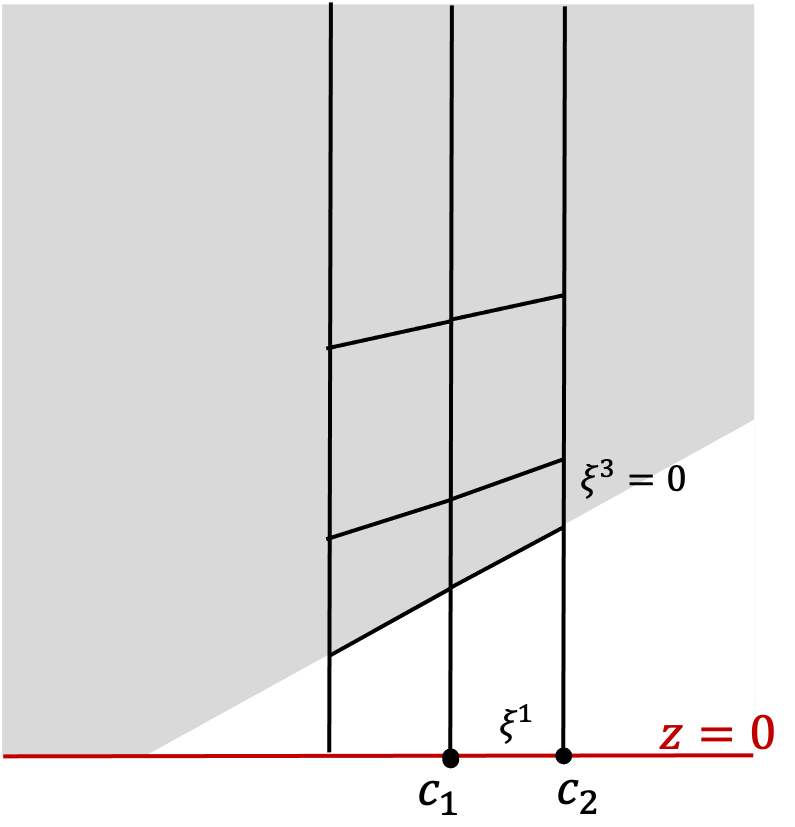
\includegraphics[width=0.45 \textwidth]{CLIMA-numerics/figures/Cartesian-localmap.png}~~~
    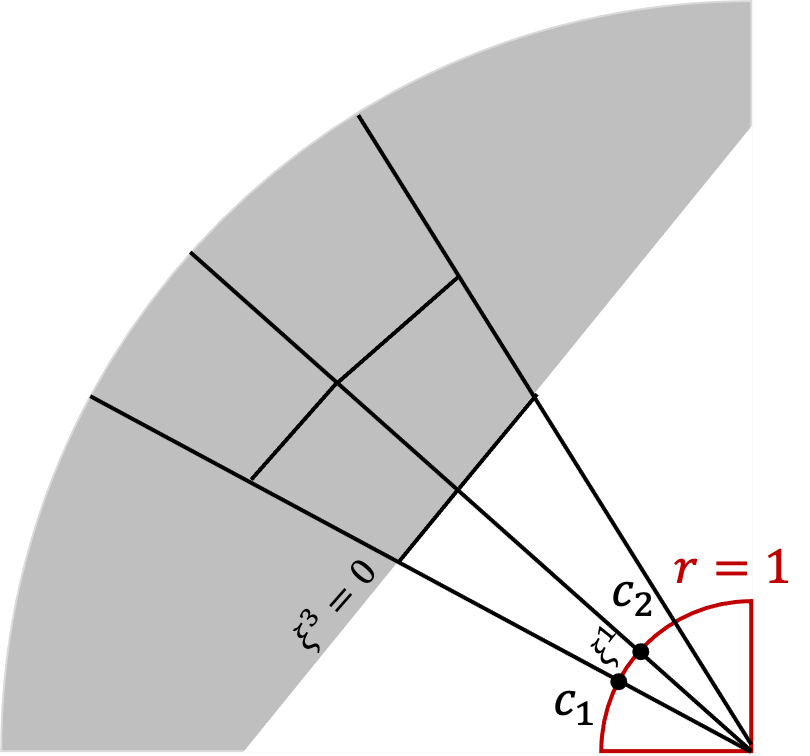
\includegraphics[width=0.45 \textwidth]{CLIMA-numerics/figures/Sphere-localmap.png}
    \caption{2D schematics of the conforming quadrilateral grid mapping $\mathbf{x}(\boldsymbol{\xi}; m)$ for each single element stack extruded by $\vb{c}_1, \vb{c}_2$ for box (left) and sphere (right) domains.}
    \label{fig:conformingmapping}
\end{figure}


% Most approaches use the equidistant central projection \citep{Sadourny1972}, the equiangular central projection \citep{Rancic1996}, or their combination \citep{Fournier2014}. All three of these approaches were compared in \citep{Nair2005}, where the equiangular mapping was found to be the most accurate. However, all three aforementioned projections are based on an inscribed cube and cannot correctly treat elements lying across cube edges. In particular, for an edge of such an element, the reference element maps for the two elements that share this edge may not agree, resulting in a loss of the SEM’s mimetic properties. Here, we present a map that avoids this issue by using a map local to each element. The map uses a bilinear transformation based on elements’ physical coordinates and does not make use of an inscribed cube. It is similar to the map used for triangular elements in \citep{Lauter2008}.


% In this formulation, for each quadrilateral element $\Omega_m$ on the surface of the unit sphere, we denote the map and its inverse by $\mathbf{r}(\boldsymbol{\xi};m)$ and $\boldsymbol{\xi}(\mathbf{r};m)$, respectively, where $\boldsymbol{\xi} = (\xi^1, \xi^2) \in [-1,1]^2$. To construct $\mathbf{r}(\boldsymbol{\xi};m)$, let $c_1$, $c_2$, $c_3$, and $c_4$ be Cartesian coordinates of the vertices of $\Omega_m$ with $c_1=(c_1^x,c_1^y,c_1^z)^T$ etc., and define

% \begin{equation}
% 	\mathbf{r}=\frac{\widetilde{\mathbf{r}}}{||\widetilde{\mathbf{r}}||_2}
% \end{equation}
% with

% \begin{equation}\label{eq:r-tilde}
% \widetilde{\mathbf{r}}=\frac{1}{4}((1-\xi^1)(1-\xi^2)c_1+(1+\xi^1)(1-\xi^2)c_2+(1+\xi^1)(1+\xi^2)c_3+(1-\xi^1)(1+\xi^2)c_4).
% \end{equation}
% We now give an analytical expression for the Jacobian matrix of the coordinate transformation $\mathbf{B}={\partial \mathbf{r}} / {\partial \boldsymbol{\xi}}$. The transformed area element needed to compute integrals in the weak-form of the PDE in a FEM or SEM formulation would be given by $(\det{\mathbf{B}} \text{d}\xi^1 \text{d} \xi^2)$ (note that in a LES formulation the area element would be identically equal to $1$). We use both Cartesian and longitude-latitude coordinates:

% \begin{equation}
% 	\mathbf{r}= \begin{pmatrix}\cos \lambda \cos \theta\\\sin \lambda \cos \theta \\ \sin \theta\end{pmatrix} , \text{ where } \lambda \in [0,2\pi], \, \theta \in \left[-\frac{\pi}{2},\frac{\pi}{2}\right]
% \end{equation}
% Since $\text{d}\mathbf{r}=\cos\theta \, \text{d}\lambda \, \mathbf{e}_{\lambda} + \text{d}\theta \,  \mathbf{e}_{\theta}$, it follows that

% \begin{equation}
% 	\mathbf{B}=\begin{pmatrix} \cos \theta & 0\\ 0 & 1\end{pmatrix} \frac{\partial(\lambda,\theta)}{\partial \boldsymbol{\xi}}=\begin{pmatrix} \cos \theta & 0\\ 0 & 1\end{pmatrix} \frac{\partial(\lambda,\theta)}{\partial \mathbf{r}}\frac{\partial\mathbf{r}}{\partial \boldsymbol{\xi}}.
% \end{equation}
% To avoid the singularity at the poles in the term

% \begin{equation}
% 	\begin{pmatrix} \cos \theta & 0\\ 0 & 1\end{pmatrix} \frac{\partial(\lambda,\theta)}{\partial \mathbf{r}}= \begin{pmatrix} -\sin\lambda &  \cos \lambda& 0\\ 0 & 0 & \frac{1}{\cos \theta}\end{pmatrix},
% \end{equation}
% we further decompose the term $\frac{\partial \mathbf{r}}{\partial \boldsymbol{\xi}}=\frac{\partial \mathbf{r}}{\partial \widetilde{\mathbf{r}}} \frac{\partial \widetilde{\mathbf{r}}}{\partial \boldsymbol{\xi}}$, so that we can extract a factor of $\cos \theta$ from $\frac{\partial \mathbf{r}}{\partial \widetilde{\mathbf{r}}}$. Some algebra shows

% \begin{equation}
% 	\frac{\partial \mathbf{r}}{\partial \widetilde{\mathbf{r}}}= \frac{1}{||\widetilde{\mathbf{r}}||_2}\begin{pmatrix} a_{11}& a_{12 }& a_{13}\\ a_{21}& a_{22 }& a_{23}\\ a_{31}& a_{32 }& a_{33} \end{pmatrix},
% \end{equation}
% where $a_{11} =\sin^2\lambda\cos^2\theta+\sin^2\theta$, $a_{12} =-({1}/{2})\sin 2\lambda \cos^2\theta$, $a_{13} =-({1}/{2})\cos\lambda \sin 2\theta$,  $a_{21} =-({1}/{2})\sin 2\lambda \cos^2\theta$, $a_{22} = \cos^2\lambda \cos^2\theta+\sin^2\theta$, $a_{23} =- ({1}/{2})\sin \lambda \sin 2\theta$, 
% $a_{31} =- ({1}/{2})\cos\lambda \sin 2\theta$, 
% $a_{32} =- ({1}/{2})\sin \lambda \sin 2\theta$, 
% $a_{12} = \cos^2\theta$. 
% Also,

% \begin{equation}
% \frac{\partial \widetilde{\mathbf{r}}}{\partial \boldsymbol{\xi}}= \frac{1}{4} 
% \begin{pmatrix}
% c_1^x & c_2^x & c_3^x & c_4^x \\
% c_1^y & c_2^y & c_3^y & c_4^y \\
% c_1^z & c_2^z & c_3^z & c_4^z
% \end{pmatrix}
% \begin{pmatrix}
% -1+\xi^2 & -1+\xi^1 \\
% 1-\xi^2 & -1- \xi^1 \\ 
% 1+ \xi^2 & 1+ \xi^1 \\ 
% -1- \xi^2 & 1- \xi^1
% \end{pmatrix}.
% \end{equation}
% Altogether, we have

% \begin{align}
% \mathbf{B} &= \frac{1}{||\widetilde{\mathbf{r}}||_2} \frac{1}{4} 
% \begin{pmatrix} 
% -\sin\lambda &  \cos \lambda & 0\\ 
%           0 &             0 & 1
% \end{pmatrix} 
% \cdot 
% \begin{pmatrix}
% a_{11} & a_{12 } & a_{13}\\
% a_{21} & a_{22 } & a_{23}\\ 
% \frac{a_{31}}{\cos\theta}& \frac{a_{32}}{\cos\theta}& \frac{a_{33}}{\cos\theta} 
% \end{pmatrix}\\
% &\cdot 
% \begin{pmatrix} 
% c_1^x & c_2^x & c_3^x & c_4^x \\
% c_1^y & c_2^y & c_3^y & c_4^y \\
% c_1^z & c_2^z & c_3^z & c_4^z 
% \end{pmatrix} 
% \cdot 
% \begin{pmatrix}
% -1 + \xi^2 & -1 + \xi^1 \\
% 1  - \xi^2 & -1 - \xi^1 \\ 
% 1  + \xi^2 &  1 + \xi^1 \\ 
% -1 - \xi^2 &  1 - \xi^1
% \end{pmatrix},
% \end{align}
% where

% \begin{equation}
% \widetilde{\mathbf{r}}= \frac{1}{4} 
% \begin{pmatrix} 
% c_1^x & c_2^x & c_3^x & c_4^x \\
% c_1^y & c_2^y & c_3^y & c_4^y \\
% c_1^z & c_2^z & c_3^z & c_4^z
% \end{pmatrix}
% \begin{pmatrix}
% (1 - \xi^1)(1 - \xi^2) \\ 
% (1 + \xi^1)(1 - \xi^2) \\ 
% (1 + \xi^1)(1 + \xi^2) \\ 
% (1 - \xi^1)(1 + \xi^2) 
% \end{pmatrix}.
% \end{equation}


\section{Arbitrary Quadrilateral Coordinates on the Sphere}

\subsection{Definition}
Consider the reference coordinate system for a single element stack
\begin{align}
\xi^1 &\in [-1,1] & \xi^2 &\in [-1,1] & \xi^3 & \mbox{\ as desired}
\end{align}
where $(\xi_1, \xi_2)$ lie on the reference quadrilateral element $ [-1,1]^2$, and $\xi_3$ denotes a generalized vertical coordinate. The transformation from the reference coordinates to Cartesian coordinates is
\begin{align}\label{eq:phys-to-ref-sphere}
\vb{x}(\xi^1,\xi^2,\xi^3) = r(\xi^1,\xi^2,\xi^3) \vb{r}(\xi^1,\xi^2)
\end{align}
where $r$ is the radial distance from the planet center, and $\vb{r}$ is the unit direction vector:
\begin{align}
\label{eq:vbr-sphere}
\mathbf{r}=\frac{\widetilde{\mathbf{r}}}{\sqrt{\widetilde{\vb{r}} \cdot \widetilde{\vb{r}}}}\\
\widetilde{\vb{r}}=\frac{1}{4} \left[ (1-\xi^1)(1-\xi^2) \vb{c}_1+(1+\xi^1)(1-\xi^2) \vb{c}_2+(1+\xi^1)(1+\xi^2) \vb{c}_3+(1-\xi^1)(1+\xi^2) \vb{c}_4 \right]\\
\vb{c}_i = c_{i,x} \vb{i} + c_{i,y} \vb{j} + c_{i,z} \vb{k}
\end{align}

The $\vb{c}_i$ should satisfy $\vb{c}_i \cdot \vb{c}_i = 1$ and be in counter-clockwise order around the quadrilateral when viewed from above.
And $\{\vb{c}_1, \vb{c}_2, \vb{c}_3, \vb{c}_4\}$ on the unit sphere defines the single element stack.

\subsection{Covariant Basis Vectors}

\begin{align}
\vb{g}_{i} = \pdiff{\vb{x}}{\xi^i} &= \pdiff{r}{\xi^i} \vb{r} + r \pdiff{\vb{r}}{\xi^i}, & \vb{g}_3 = \pdiff{\vb{x}}{\xi^3} &= \pdiff{r}{\xi^3} \vb{r},
\end{align}

\subsection{Covariant Metric Terms}

\begin{align}
\pdiff{\vb{r}}{\xi^i} &= (\tilder \cdot \tilder)^{-3/2} \left[ \pdiff{\tilder}{\xi^i} (\tilder \cdot \tilder) - \tilder \left( \pdiff{\tilder}{\xi^i} \cdot \tilder \right) \right]
\end{align}
\begin{align}
\pdiff{\tilder}{\xi^1} &= \frac{(1-\xi^2)}{4} (\vb{c}_2 - \vb{c}_1) + \frac{(1 + \xi^2)}{4} (\vb{c}_3 - \vb{c}_4) \\
\pdiff{\tilder}{\xi^2} &= \frac{(1-\xi^1)}{4} (\vb{c}_4 - \vb{c}_1) + \frac{(1 + \xi^1)}{4} (\vb{c}_3 - \vb{c}_2)
\end{align}
\begin{align}
\vb{r} \cdot \pdiff{\vb{r}}{\xi^i} &= (\tilder \cdot \tilder)^{-2} \left[ \left( \pdiff{\tilder}{\xi^i} \cdot \tilder \right) (\tilder \cdot \tilder) - (\tilder \cdot \tilder) \left( \pdiff{\tilder}{\xi^i} \cdot \tilder \right) \right] = 0 \\
\pdiff{\vb{r}}{\xi^i} \cdot \pdiff{\vb{r}}{\xi^j} &= (\tilder \cdot \tilder)^{-2} \left[ \left( \pdiff{\tilder}{\xi^i} \cdot \pdiff{\tilder}{\xi^j} \right) (\tilder \cdot \tilder) - \left( \pdiff{\tilder}{\xi^i} \cdot \tilder \right) \left( \pdiff{\tilder}{\xi^j} \cdot \tilder \right) \right]
\end{align}


Let denote $i,j \in \{1,2\}$, we have
\begin{align}
\label{eq:g-sphere}
g_{33} = \pdiff{\vb{x}}{\xi^3} \cdot \pdiff{\vb{x}}{\xi^3} &= \left( \pdiff{r}{\xi^3} \right)^2 \\
g_{3 i} = \pdiff{\vb{x}}{\xi^3} \cdot \pdiff{\vb{x}}{\xi^i} &= \pdiff{r}{\xi^3} \cdot \pdiff{r}{\xi^i} \\
g_{ij} = \pdiff{\vb{x}}{\xi^i} \cdot \pdiff{\vb{x}}{\xi^j} &= \left( \pdiff{r}{\xi^i} \cdot \pdiff{r}{\xi^j} \right) + r^2 \left( \pdiff{\vb{r}}{\xi^i} \cdot \pdiff{\vb{r}}{\xi^j} \right)
\end{align}

\subsection{Metric Determinant}

\begin{align}
\sqrt{g} = \left( \pdiff{r}{\xi^3} \right) r^2 \left[ \left( \pdiff{\vb{r}}{\xi^1} \cdot \pdiff{\vb{r}}{\xi^1} \right) \left( \pdiff{\vb{r}}{\xi^2} \cdot \pdiff{\vb{r}}{\xi^2} \right) - \left( \pdiff{\vb{r}}{\xi^1} \cdot \pdiff{\vb{r}}{\xi^2} \right)^2 \right]^{1/2}
\end{align}


\subsection{Velocity Transformations}

Given that most test cases on the sphere are specified in spherical coordinates, it is useful to know how to transform vectors from spherical coordinates to Cartesian coordinates.

\begin{align}
r &\in [0, \infty) & \lambda &\in [0,2\pi) & \phi &\in [-\pi/2,\pi/2]
\end{align}
Forward transforms:
\begin{align}
r &= \sqrt{x^2 + y^2 + z^2} \\
\lambda &= \mathrm{arctan2}(y,x) \\
\phi &= \mathrm{arcsin}(z)
\end{align}
Reverse transforms:
\begin{align}
x &= r \cos \lambda \cos \phi \\
y &= r \sin \lambda \cos \phi \\
z &= r \sin \phi
\end{align}
Unit vectors:
\begin{align}
\vb{e}_r &= (\cos \lambda \cos \phi) \vb{i} + (\sin \lambda \cos \phi) \vb{j} + (\sin \phi) \vb{k} \\
\vb{e}_\lambda &= (- \sin \lambda) \vb{i} + (\cos \lambda) \vb{j} \\
\vb{e}_\phi &= (-\cos \lambda \sin \phi) \vb{i} + (-\sin \lambda \sin \phi) \vb{j} + (\cos \phi) \vb{k}
\end{align}
Transformation to Cartesian:
\begin{align}
\left( \begin{array}{c} u_x \\ u_y \\ u_z \end{array} \right) = \left( \begin{array}{ccc} \cos \lambda \cos \phi & - \sin \lambda & - \cos \lambda \sin \phi \\ \sin \lambda \cos \phi & \cos \lambda & - \sin \lambda \sin \phi \\ \sin \phi & 0 & \cos \phi \end{array} \right) \left( \begin{array}{c} u_r \\ u_\lambda \\ u_\phi \end{array} \right)
\end{align}
Transformation to Covariant Arbitrary Quadrilateral Coords:
\begin{align}
u_i &= \vb{u} \cdot \vb{g}_i & \mbox{(Definition of covariant components)}
\end{align}
\begin{align}
\left( \begin{array}{c} u_1 \\ u_2 \\ u_3 \end{array} \right) 
&= \left( \begin{array}{ccc} \pdiff{r}{\xi^1} & r \left( \vb{e}_\lambda \cdot \pdiff{\vb{r}}{\xi^1} \right) & r \left( \vb{e}_\phi \cdot \pdiff{\vb{r}}{\xi^1} \right)  \\
[2.0ex]  \pdiff{r}{\xi^2} & r \left( \vb{e}_\lambda \cdot \pdiff{\vb{r}}{\xi^2} \right) & r \left( \vb{e}_\phi \cdot \pdiff{\vb{r}}{\xi^2} \right) \\
[2.0ex] \pdiff{r}{\xi^3}  & 0 & 0 \end{array} \right) \left( \begin{array}{c} u_r \\ u_\lambda \\ u_\phi   \end{array} \right) \\
\end{align}

Transformation to Covariant Arbitrary Quadrilateral Coords on the Sphere:
\begin{align}
\label{eq:cov-cartesian-sphere}
\left( \begin{array}{c} u_1 \\ u_2 \\ u_3 \end{array} \right) 
&= \left( \begin{array}{ccc} \vb{e}_x\cdot\left(\pdiff{r}{\xi^1}\vb{r} + r \pdiff{\vb{r}}{\xi^1}\right) & \vb{e}_y\cdot\left(\pdiff{r}{\xi^1}\vb{r} + r \pdiff{\vb{r}}{\xi^1}\right) & \vb{e}_z\cdot\left(\pdiff{r}{\xi^1}\vb{r} + r \pdiff{\vb{r}}{\xi^1}\right)  \\
[2.0ex]  \vb{e}_x\cdot\left(\pdiff{r}{\xi^2}\vb{r} + r \pdiff{\vb{r}}{\xi^2}\right) & \vb{e}_y\cdot\left(\pdiff{r}{\xi^2}\vb{r} + r \pdiff{\vb{r}}{\xi^2}\right) & \vb{e}_z\cdot\left(\pdiff{r}{\xi^2}\vb{r} + r \pdiff{\vb{r}}{\xi^2}\right) \\
[2.0ex] \vb{e}_x\cdot\left(\pdiff{r}{\xi^3}\vb{r} \right) & \vb{e}_y\cdot\left(\pdiff{r}{\xi^3}\vb{r} \right) & \vb{e}_z\cdot\left(\pdiff{r}{\xi^3}\vb{r} \right) 
\end{array}\right) \left( \begin{array}{c} u_x \\ u_y \\ u_z   \end{array} \right)
\end{align}

\section{Arbitrary Quadrilateral Coords in Cartesian Geometry}

\subsection{Definition}

In this case we don't project the quadrilateral point to the sphere, but otherwise things are similar. The transformation from the reference coordinates in the single element stack to Cartesian coordinates is

\begin{align}\label{eq:phys-to-ref-cartesian}
\vb{x}(\xi^1,\xi^2,\xi^3) = r(\xi^1,\xi^2,\xi^3) \vb{k} + \tilder(\xi^1,\xi^2)
\end{align}
where $r$ is the height with direction vector $\vb{k}$, $\tilder$ is horizontal position vector:
\begin{align}
\label{eq:vbr-cartesian}
\tilder=\frac{1}{4} \left[ (1-\xi^1)(1-\xi^2) \vb{c}_1+(1+\xi^1)(1-\xi^2) \vb{c}_2+(1+\xi^1)(1+\xi^2) \vb{c}_3+(1-\xi^1)(1+\xi^2) \vb{c}_4 \right]\\
\vb{c}_i = c^x_i \vb{i} + c^y_i \vb{j}
\end{align}
here  $\vb{c}_i$ satisfy $\vb{c}_i \cdot \vb{k} = 0$ and be in counter-clockwise order around the quadrilateral when viewed from above.
And $\{\vb{c}_1, \vb{c}_2, \vb{c}_3, \vb{c}_4\}$ denotes the single element stack.


\subsection{Covariant Metric Terms}
\begin{align}
\pdiff{\vb{x}}{\xi^3} &= \pdiff{r}{\xi^3} \vb{k}, & \pdiff{\vb{x}}{\xi^i} &= \pdiff{r}{\xi^i} \vb{k} + \pdiff{\tilder}{\xi^i}
\end{align}
\begin{align}
\vb{k} \cdot \tilder &= 0, & \vb{k} \cdot \pdiff{\tilder}{\xi^i} &= 0
\end{align}

Let denote $i,j \in \{1,2\}$, we have
\begin{align}
\label{eq:g-cartesian}
g_{33} = \pdiff{\vb{x}}{\xi^3} \cdot \pdiff{\vb{x}}{\xi^3} &= \left( \pdiff{r}{\xi^3} \right)^2 \\
g_{3 i} = \pdiff{\vb{x}}{\xi^3} \cdot \pdiff{\vb{x}}{\xi^i} &= \pdiff{r}{\xi^3} \cdot \pdiff{r}{\xi^i} \\
g_{ij} = \pdiff{\vb{x}}{\xi^i} \cdot \pdiff{\vb{x}}{\xi^j} &= \left( \pdiff{r}{\xi^i} \cdot \pdiff{r}{\xi^j} \right) + \left( \pdiff{\tilder}{\xi^i} \cdot \pdiff{\tilder}{\xi^j} \right)
\end{align}


\subsection{Metric Determinant}

\begin{align}
\sqrt{g} &= \left( \pdiff{r}{\xi^3} \right) \left[ \left( \pdiff{\tilder}{\xi^1} \cdot \pdiff{\tilder}{\xi^1} \right) \left( \pdiff{\tilder}{\xi^2} \cdot \pdiff{\tilder}{\xi^2} \right) - \left( \pdiff{\tilder}{\xi^1} \cdot \pdiff{\tilder}{\xi^2} \right)^2 \right]^{1/2}
\end{align}

\subsection{Velocity Transformations}
Transformation to Covariant Arbitrary Quadrilateral Coords in Cartesian Geometry:
\begin{align}
\label{eq:cov-cartesian-cartesian}
\left( \begin{array}{c} u_1 \\ u_2 \\ u_3 \end{array} \right) 
&= \left( \begin{array}{ccc} \vb{e}_x\cdot\left(\pdiff{\tilder}{\xi^1}\right) & \vb{e}_y\cdot\left(\pdiff{\tilder}{\xi^1}\right) & \pdiff{r}{\xi^1} + \vb{e}_z\cdot\left(  \pdiff{\tilder}{\xi^1}\right)  \\
[2.0ex]  \vb{e}_x\cdot\left(\pdiff{\tilder}{\xi^2}\right) & \vb{e}_y\cdot\left(\pdiff{\tilder}{\xi^2}\right) & \pdiff{r}{\xi^2} + \vb{e}_z\cdot\left( \pdiff{\tilder}{\xi^2}\right) \\
[2.0ex] 0& 0 & \pdiff{r}{\xi^3}  
\end{array}\right) \left( \begin{array}{c} u_x \\ u_y \\ u_z   \end{array} \right)
\end{align}

\section{Bubble correction}

Correction so that the integration of the domain gives the exact area of the sphere: this can be done by scaling the metric terms on the interior of the domain.

\section{Implementation}
\begin{enumerate}
    \item build cubed sphere mesh
    \item assign each single element stack a quadrilateral $\vb{c}_1, \vb{c}_2, \vb{c}_3, \vb{c}_4$
    \item  $\xi^3 \in [0, 1]$
    \item compute $r$, $\xi^1$, $\xi^2$, $\xi^3$ from mesh at each nodal point 
    \item compute analytically $\vb{r}$~($\widetilde{\vb{r}}$) following \eqref{eq:vbr-sphere} and \eqref{eq:vbr-cartesian} its derivatives with respect to $\xi^1$ and $\xi^2$ at each nodal point 
    \item compute derivatives of $r$ with respect to $\xi^1$, $\xi^2$, $\xi^3$ numerically in each element at each nodal point \hl{DH: not sure it is continuous at the element edges}
    \item compute $g_{ij}$ following~\eqref{eq:g-sphere}\eqref{eq:g-cartesian} 
    \item compute the transformation matrix between Covariant Arbitrary Quadrilateral Coords and Cartesian Coords following \eqref{eq:cov-cartesian-sphere}  \eqref{eq:cov-cartesian-cartesian} 
\end{enumerate}



%%%%%%%%%%%%%%%%%%%%%%%%%%%%%%%% Old Equidistant & Equiangular Mapping section %%%%%%%%%%%%%%%%%%%%%%%%%%
% Need to extract only relevant parts on equiangular coord to general quadirangular coord  transformation
% part now

\section{Equiangular Cubed Sphere Mesh}\label{s:cubed_sphere_transform}
\label{s:equiangle_cubed_sphere_transform}


In this section, we discuss how the general conforming quadrilateral representation relates to the cubed-sphere coordinates, when we need to specify the mapping presented in \eqref{eq:phys-to-ref-sphere} and \eqref{eq:vbr-sphere}.

% represent vector fields within reference elements on a cubed-sphere mesh with a generalized vertical coordinate. We follow \cite{Nair2005} in the treatment of the horizontal (tangential) directions along spherical shells, but generalize their treatment to spherical shells with radii $r$ that increase outward from the center of the planet (i.e., for a deep atmosphere).

We consider a sphere of radius $r$ that is decomposed into six identical regions, obtained by central projection of the faces of an inscribed cube onto the spherical surface. Each of the six local coordinate systems is free of singularites and employs identical metric terms, thus creating a non-orthogonal curvilinear coordinate system on the surface of the sphere. The center of the inscribed cube coincides with the center of the sphere. 
\begin{figure}
    \centering
    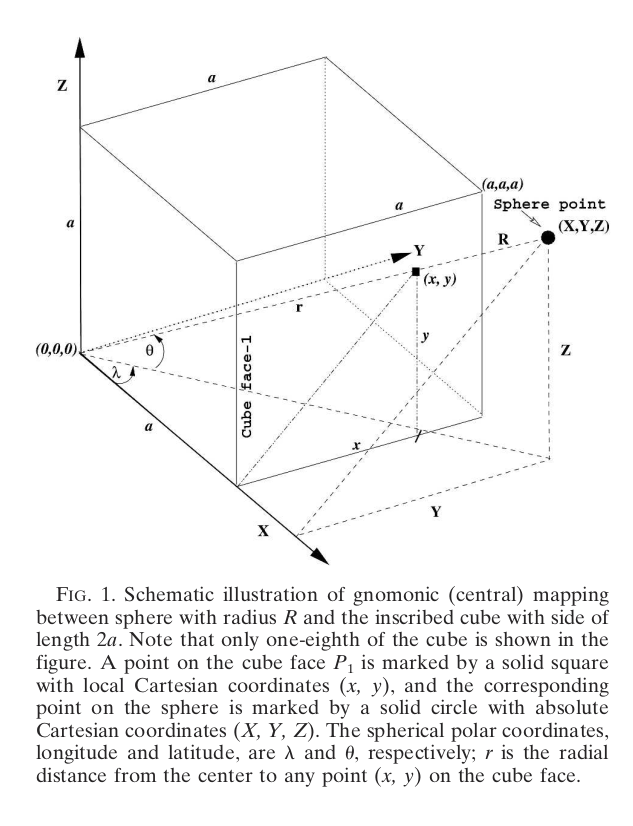
\includegraphics[scale=0.4,trim=0cm 9cm 0cm 0cm, clip]{CLIMA-atmos/figures/numerics/NairFig1.png}
    \caption{One octant of inscribed cube and one quadrant of cube face $P_1$ (from \cite{Nair2005}). Note that $(X,Y,Z)$ in the figure corresponds to $(x,y,z)$ in the text, and $(x,y)$ in the figure corresponds to $(\xi^1,\xi^2)$.}
    \label{fig:NairFig1}
\end{figure}

\begin{figure}
    \centering
    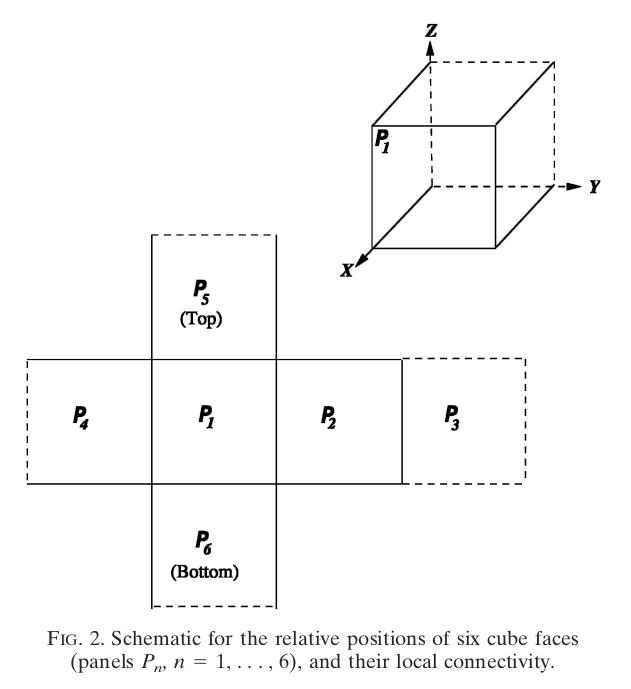
\includegraphics[scale=0.4]{CLIMA-atmos/figures/numerics/NairFig2.png}
    \caption{Relative positions of the six cube faces ($P^n$, $n=1, \dots, 6$) and their local connectivity. (From \cite{Nair2005}. The top-right cube represents only one octant of the cube and one quadrant of the $P^1$ face. The reader should be aware that currently the cube face labelling presented in this figure does not reflect the internal numbering we have in ClimateMachine. }
    \label{fig:NairFig2}
\end{figure}

We assume a Cartesian coordinate system for the Euclidean space in which the sphere and inscribed cube are embedded, with coordinates $(x^1, x^2, x^3) = (x, y, z)$ and associated coordinate vectors directed normal to the faces of the cube; the coordinate origin is at the collocated centers of the cube and sphere (and the $z$ coordinate is not to be confused with the altitude $z$ we defined previously). See Fig.~\ref{fig:NairFig1}. Let $(\xi^1, \xi^2)$ be local coordinates on the surface of each cube face (labeled $n=1,\dots, 6)$,  and let $(\lambda, \phi, r)$ denote the usual spherical polar coordinates with longitude  $\lambda$, latitude $\phi$, and radial distance from the planet center $r=r(\lambda, \phi, \xi^3$). The radius $r$ depends on the horizontal coordinates and a generalized vertical coordinate $\xi^3$. That is, we can view the spherical polar coordinates as functions of the generalized coordinates $(\xi^1, \xi^2, \xi^3, n)$, with longitude $\lambda = \lambda(\xi^1, \xi^2, n)$ and latitude $\phi = \phi(\xi^1, \xi^2, n)$ parameterized by $(\xi^1, \xi^2)$ for each face $n$, and $r = r(\xi^1, \xi^2, \xi^3)$ parameterized by all three generalized coordinates ($r$ will not depend on the face index $n$). Then, we can write the usual transformation from spherical polar coordinates ($\lambda, \phi, r)$ to Cartesian coordinates in the embedding space (as in section~\ref{s:example_coordinates}) as
\begin{subequations} \label{e:spherical-coords-terrain-follow}
    \begin{align}
    x &= r(\xi^1, \xi^2, \xi^3) \cos \lambda(\xi^1, \xi^2, n) \cos \phi(\xi^1, \xi^2, n) , \\
    y &= r(\xi^1, \xi^2, \xi^3) \sin \lambda(\xi^1, \xi^2, n) \cos \phi(\xi^1, \xi^2, n) , \\
    z &= r(\xi^1, \xi^2, \xi^3) \sin \phi(\xi^1, \xi^2, n).
    \end{align}
\end{subequations}
We adopt the convention that lateral faces of the cube (normal to the $x$ and $y$ axes) are labeled $n=1, \dots, 4$; the top and bottom faces (normal to the $z$ axis) are labeled as $n=5$ and $n=6$, respectively (Fig.~\ref{fig:NairFig2}).


% \section{Equidistant Cubed-Sphere Mesh}\label{s:cubed_sphere_transform}

% Let $P^1$ be the cube face with $x$ as the normal direction going from the center through the prime meridian, and consider the first positive octant of the cube. If we adopt local Cartesian coordinates centered on the cube face, so that $(\xi^1, \xi^2) \in [-1, 1]$, the following trigonometric relations hold for $n=1$ (Fig.~\ref{fig:NairFig1}):
% \begin{equation}\label{e:cube-radial-distance-and-coords}
%     \sin \phi = \frac{z}{r}, \quad \tan \lambda = \xi^1 = \frac{y}{x}, \quad \text{and} \quad \frac{y}{z} = \frac{\xi^1}{\xi^2}. 
% \end{equation}
% From the above relations and \eqref{e:spherical-coords-terrain-follow}, we have that
% \begin{subequations} \label{e:P1-sphere-to-cube}
%     \begin{align}
%         \xi^1 &= \tan \lambda,\\
%         \xi^2 &= \tan \phi \sec \lambda .
%     \end{align}
% \end{subequations}
% Equations \eqref{e:P1-sphere-to-cube} give the basic gnomonic transformation between the cube and its circumscribing sphere. In this nondimensional form, the transformations from longitude and latitude to the local coordinates $\xi^1$ and $\xi^2$ on the cube faces do not depend on $r$; thus, $(\xi^1, \xi^2)$ parameterize $(\lambda, \phi)$ for any spherical surface of radius $r$.

% Relations analogous to \eqref{e:P1-sphere-to-cube} hold for the other faces of the cube and can be obtained by rotation of the spherical polar coordinate system. Given the mappings $(\xi^1, \xi^2) \rightarrow (\lambda, \phi)$ for the horizontal coordinates on the surface of the spherical shells, we can obtain the mappings for the 3D coordinates $(\xi^2, \xi^2, \xi^3) \rightarrow (x, y, z)$ from \eqref{e:spherical-coords-terrain-follow}.

% To obtain the mappings, we use the nondimensional radial distance $r_c$ from a point with local Cartesian coordinates ($\xi^1, \xi^2$) on the face of the cube to the center of the cube, with  
% \[
% r_c^2 = 1 + (\xi^1)^2 + (\xi^2)^2.
% \]
% The results for the 6 cube faces, with $r=r(\xi^1, \xi^2, \xi^3)$ understood to depend on all three generalized coordinates, are as follows \citep[cf.][]{Nair2005}.

% \begin{enumerate}
% \item For $P^1$ $\left(-\frac{\pi}{4} \leq \lambda \leq  \frac{\pi}{4}, \quad -\frac{\phi}{4} \leq \lambda \leq  \frac{\phi}{4} \right)$: 
% \begin{equation}
%   \begin{array}{l}
%         \xi^1 = \tan \lambda,\\
%         \xi^2 = \tan \phi \sec \lambda ,
%   \end{array}
% \end{equation}
% and
% \begin{equation}\label{e:P1-cube-to-global-and-vice-versa}
%     \begin{array}{l}
%         x = r/r_c,  \\
%         y = (r/r_c) \xi^1,\\
%         z = (r/r_c) \xi^2,
%     \end{array}
%     \qquad 
%     \begin{array}{l}
%          \xi^1 = {y}/{x}, \\
%          \xi^2 = {z}/{x} .\\
%     \end{array}
% \end{equation}
% % and
% % \begin{equation}
% % \vec{b}_1 = 
% %     \begin{bmatrix}
% %         r\frac{-\xi^1}{r_c^3} + \frac{\partial r}{\partial \xi^1}\frac{1}{r_c}  \\
% %         r(\frac{1}{r_c} - \frac{(\xi^1)^2}{r_c^3})+ \frac{\partial r}{\partial \xi^1}\frac{\xi^1}{r_c} \\
% %         r( - \frac{\xi^1 \xi^2}{r_c^3})+ \frac{\partial r}{\partial \xi^2}\frac{\xi^2}{r_c} \\
% %     \end{bmatrix}
% % \qquad 
% % \vec{b}_2 = 
% %     \begin{bmatrix}
% %         r\frac{-\xi^2}{r_c^3} + \frac{\partial r}{\partial \xi^2}\frac{1}{r_c}  \\
% %         r( - \frac{\xi^1 \xi^2}{r_c^3})+ \frac{\partial r}{\partial \xi^2}\frac{\xi^1}{r_c} \\
% %         r(\frac{1}{r_c} - \frac{(\xi^2)^2}{r_c^3})+ \frac{\partial r}{\partial \xi^2}\frac{\xi^2}{r_c} \\
% %     \end{bmatrix}
% % \qquad 
% % \vec{b}_3 = 
% %     \begin{bmatrix}
% %         \frac{\partial r}{\partial \xi^3}\frac{1}{r_c}  \\
% %         \frac{\partial r}{\partial \xi^3}\frac{\xi^1}{r_c}\\
% %         \frac{\partial r}{\partial \xi^3}\frac{\xi^2}{r_c}\\
% %     \end{bmatrix}
% % \end{equation}

% \item For $P^2$ $\left(\frac{\pi}{4} \leq \lambda \leq  \frac{3\pi}{4}, \quad -\frac{\phi}{4} \leq \lambda \leq  \frac{\phi}{4} \right)$:
% \begin{equation}
% \begin{split} \label{e:P2-sphere-to-cube}
%         \xi^1 &= - \cot \lambda ,\\
%         \xi^2 &= \tan \phi \csc \lambda ,
% \end{split}
% \end{equation}
% and
% \begin{equation}\label{e:P2-cube-to-global-and-vice-versa}
%     \begin{array}{l}
%         x = -(r/r_c) \xi^1 , \\
%         y = (r/r_c),\\
%         z = (r/r_c) \xi^2,
%     \end{array}
% \qquad
%     \begin{array}{l}
%         \xi^1 = -{x}/{y}, \\
%         \xi^2 =  {z}/{y} .\\
%     \end{array}
% \end{equation}
% % and
% % \begin{equation}
% % \vec{b}_1 = 
% %     \begin{bmatrix}
% %         -r(\frac{1}{r_c} - \frac{(\xi^1)^2}{r_c^3}) -\frac{\partial r}{\partial \xi^1}\frac{\xi^1}{r_c} \\
% %         r\frac{-\xi^1}{r_c^3} + \frac{\partial r}{\partial \xi^1}\frac{1}{r_c}  \\
% %         r( - \frac{\xi^1 \xi^2}{r_c^3})+ \frac{\partial r}{\partial \xi^2}\frac{\xi^2}{r_c} \\
% %     \end{bmatrix}
% % \qquad 
% % \vec{b}_2 = 
% %     \begin{bmatrix}
% %         -r( - \frac{\xi^1 \xi^2}{r_c^3}) - \frac{\partial r}{\partial \xi^2}\frac{\xi^1}{r_c} \\
% %         r\frac{-\xi^2}{r_c^3} + \frac{\partial r}{\partial \xi^2}\frac{1}{r_c}  \\
% %         r(\frac{1}{r_c} - \frac{(\xi^2)^2}{r_c^3})+ \frac{\partial r}{\partial \xi^2}\frac{\xi^2}{r_c} \\
% %     \end{bmatrix}
% % \qquad 
% % \vec{b}_3 = 
% %     \begin{bmatrix}
% %         -\frac{\partial r}{\partial \xi^3}\frac{\xi^1}{r_c}\\
% %         \frac{\partial r}{\partial \xi^3}\frac{1}{r_c}  \\
% %         \frac{\partial r}{\partial \xi^3}\frac{\xi^2}{r_c}\\
% %     \end{bmatrix}
% % \end{equation}
% \item For $P^3$ $\left(\frac{3\pi}{4} \leq \lambda \leq  \frac{5\pi}{4}, \quad -\frac{\phi}{4} \leq \lambda \leq  \frac{\phi}{4} \right)$:
% \begin{equation} \label{e:P3-sphere-to-cube}
%     \begin{array}{l}
%         \xi^1 = - \tan \lambda ,\\
%         \xi^2 = - \tan \phi \sec \lambda ,
%     \end{array}
% \end{equation}
% and
% \begin{equation}\label{e:P3-cube-to-global-and-vice-versa}
%     \begin{array}{l}
%         x = -(r/r_c),  \\
%         y = -(r/r_c) \xi^1,\\
%         z = (r/r_c) \xi^2,
%     \end{array}
%     \qquad 
%     \begin{array}{l}
%         \xi^1 = {y}/{x}, \\
%         \xi^2 = - {z}/{x} .\\
%     \end{array}
% \end{equation}
% % and
% % \begin{equation}
% % \vec{b}_1 = 
% %     \begin{bmatrix}
% %         -r\frac{-\xi^1}{r_c^3} - \frac{\partial r}{\partial \xi^1}\frac{1}{r_c}  \\
% %         -r(\frac{1}{r_c} - \frac{(\xi^1)^2}{r_c^3})- \frac{\partial r}{\partial \xi^1}\frac{\xi^1}{r_c} \\
% %         r( - \frac{\xi^1 \xi^2}{r_c^3})+ \frac{\partial r}{\partial \xi^2}\frac{\xi^2}{r_c} \\
% %     \end{bmatrix}
% % \qquad 
% % \vec{b}_2 = 
% %     \begin{bmatrix}
% %         -r\frac{-\xi^2}{r_c^3} - \frac{\partial r}{\partial \xi^2}\frac{1}{r_c}  \\
% %         -r( - \frac{\xi^1 \xi^2}{r_c^3})- \frac{\partial r}{\partial \xi^2}\frac{\xi^1}{r_c} \\
% %         r(\frac{1}{r_c} - \frac{(\xi^2)^2}{r_c^3})+ \frac{\partial r}{\partial \xi^2}\frac{\xi^2}{r_c} \\
% %     \end{bmatrix}
% % \qquad 
% % \vec{b}_3 = 
% %     \begin{bmatrix}
% %         -\frac{\partial r}{\partial \xi^3}\frac{1}{r_c}  \\
% %         -\frac{\partial r}{\partial \xi^3}\frac{\xi^1}{r_c}\\
% %         \frac{\partial r}{\partial \xi^3}\frac{\xi^2}{r_c}\\
% %     \end{bmatrix}
% % \end{equation}


% \item For $P^4$ $\left(\frac{5\pi}{4} \leq \lambda \leq  \frac{7\pi}{4}, \quad -\frac{\phi}{4} \leq \lambda \leq  \frac{\phi}{4} \right)$:
% \begin{equation} \label{e:P4-sphere-to-cube}
%     \begin{array}{l}
%         \xi^1 = - \cot \lambda ,\\
%         \xi^2 = - \tan \phi \csc \lambda ,
%     \end{array}
% \end{equation}
% and
% \begin{equation}\label{e:P4-cube-to-global-and-vice-versa}
%     \begin{array}{l}
%         x = (r/r_c) \xi^1,  \\
%         y = -(r/r_c),\\
%         z = (r/r_c) \xi^2,
%     \end{array}
%     \qquad
%     \begin{array}{l}
%         \xi^1 = -{x}/{y}, \\
%         \xi^2 = -{z}/{y} .\\
%     \end{array}
% \end{equation}
% % and
% % \begin{equation}
% % \vec{b}_1 = 
% %     \begin{bmatrix}
% %         r(\frac{1}{r_c} - \frac{(\xi^1)^2}{r_c^3}) +\frac{\partial r}{\partial \xi^1}\frac{\xi^1}{r_c} \\
% %         -r\frac{-\xi^1}{r_c^3} - \frac{\partial r}{\partial \xi^1}\frac{1}{r_c}  \\
% %         r( - \frac{\xi^1 \xi^2}{r_c^3})+ \frac{\partial r}{\partial \xi^2}\frac{\xi^2}{r_c} \\
% %     \end{bmatrix}
% % \qquad 
% % \vec{b}_2 = 
% %     \begin{bmatrix}
% %         r( - \frac{\xi^1 \xi^2}{r_c^3}) + \frac{\partial r}{\partial \xi^2}\frac{\xi^1}{r_c} \\
% %         -r\frac{-\xi^2}{r_c^3} + \frac{\partial r}{\partial \xi^2}\frac{1}{r_c}  \\
% %         r(\frac{1}{r_c} - \frac{(\xi^2)^2}{r_c^3})+ \frac{\partial r}{\partial \xi^2}\frac{\xi^2}{r_c} \\
% %     \end{bmatrix}
% % \qquad 
% % \vec{b}_3 = 
% %     \begin{bmatrix}
% %         \frac{\partial r}{\partial \xi^3}\frac{\xi^1}{r_c}\\
% %         -\frac{\partial r}{\partial \xi^3}\frac{1}{r_c}  \\
% %         \frac{\partial r}{\partial \xi^3}\frac{\xi^2}{r_c}\\
% %     \end{bmatrix}
% % \end{equation}

% \item For $P^5$ $\left(\pi/4 \leq \phi \leq \pi/2 \right)$:
% \begin{equation} \label{e:P5-sphere-to-cube}
%     \begin{array}{l}
%         \xi^1 = - \sin \lambda \cot \phi ,\\
%         \xi^2 = - \cos \lambda \cot \phi , 
%     \end{array}
% \end{equation}
% and
% \begin{equation}\label{e:P5-cube-to-global-and-vice-versa}
%     \begin{array}{l}
%         x = - (r/r_c) \xi^2,  \\
%         y = (r/r_c) \xi^1,\\
%         z = (r/r_c),
%     \end{array}
%     \qquad
%     \begin{array}{l}
%         \xi^1 = {y}/{z}, \\
%         \xi^2 = -{x}/{z} .\\
%     \end{array}
% \end{equation}
% % and
% % \begin{equation}
% % \vec{b}_1 = 
% %     \begin{bmatrix}
% %         -r( - \frac{\xi^1 \xi^2}{r_c^3})- \frac{\partial r}{\partial \xi^2}\frac{\xi^2}{r_c} \\
% %         r(\frac{1}{r_c} - \frac{(\xi^1)^2}{r_c^3}) +\frac{\partial r}{\partial \xi^1}\frac{\xi^1}{r_c} \\
% %         r\frac{-\xi^1}{r_c^3} + \frac{\partial r}{\partial \xi^1}\frac{1}{r_c}  \\
% %     \end{bmatrix}
% % \qquad 
% % \vec{b}_2 = 
% %     \begin{bmatrix}
% %         -r(\frac{1}{r_c} - \frac{(\xi^2)^2}{r_c^3}) - \frac{\partial r}{\partial \xi^2}\frac{\xi^2}{r_c} \\
% %         r( - \frac{\xi^1 \xi^2}{r_c^3}) + \frac{\partial r}{\partial \xi^2}\frac{\xi^1}{r_c} \\
% %         r\frac{-\xi^2}{r_c^3} + \frac{\partial r}{\partial \xi^2}\frac{1}{r_c}  \\
% %     \end{bmatrix}
% % \qquad 
% % \vec{b}_3 = 
% %     \begin{bmatrix}
% %         -\frac{\partial r}{\partial \xi^3}\frac{\xi^2}{r_c}\\
% %         \frac{\partial r}{\partial \xi^3}\frac{\xi^1}{r_c}\\
% %         \frac{\partial r}{\partial \xi^3}\frac{1}{r_c}  \\
% %     \end{bmatrix}
% % \end{equation}

% \item For $P^6$ $\left(-\pi/2 \leq \phi \leq -\pi/4 \right)$:
% \begin{equation} \label{e:P6-sphere-to-cube}
%     \begin{array}{l}
%         \xi^1 = - \sin \lambda \cot \phi ,\\
%         \xi^2 = -\cos \lambda \cot \phi ,
%     \end{array}
% \end{equation}
% and
% \begin{equation}\label{e:P6-cube-to-global-and-vice-versa}
%     \begin{array}{l}
%         x = (r/r_c) \xi^2,  \\
%         y = (r/r_c)\xi^1,\\
%         z = -(r/r_c),
%     \end{array}
%     \qquad
%     \begin{array}{l}
%         \xi^1 = -{y}/{z}, \\
%         \xi^2 = -{x}/{z}. \\
%     \end{array}
% \end{equation}
% % and
% % \begin{equation}
% % \vec{b}_1 = 
% %     \begin{bmatrix}
% %         r( - \frac{\xi^1 \xi^2}{r_c^3})+ \frac{\partial r}{\partial \xi^2}\frac{\xi^2}{r_c} \\
% %         r(\frac{1}{r_c} - \frac{(\xi^1)^2}{r_c^3}) +\frac{\partial r}{\partial \xi^1}\frac{\xi^1}{r_c} \\
% %         -r\frac{-\xi^1}{r_c^3} - \frac{\partial r}{\partial \xi^1}\frac{1}{r_c}  \\
% %     \end{bmatrix}
% % \qquad 
% % \vec{b}_2 = 
% %     \begin{bmatrix}
% %         r(\frac{1}{r_c} - \frac{(\xi^2)^2}{r_c^3}) + \frac{\partial r}{\partial \xi^2}\frac{\xi^2}{r_c} \\
% %         r( - \frac{\xi^1 \xi^2}{r_c^3}) + \frac{\partial r}{\partial \xi^2}\frac{\xi^1}{r_c} \\
% %         -r\frac{-\xi^2}{r_c^3} + \frac{\partial r}{\partial \xi^2}\frac{1}{r_c}  \\
% %     \end{bmatrix}
% % \qquad 
% % \vec{b}_3 = 
% %     \begin{bmatrix}
% %         \frac{\partial r}{\partial \xi^3}\frac{\xi^2}{r_c}\\
% %         \frac{\partial r}{\partial \xi^3}\frac{\xi^1}{r_c}\\
% %         -\frac{\partial r}{\partial \xi^3}\frac{1}{r_c}  \\
% %     \end{bmatrix}
% % \end{equation}
% \end{enumerate}

% In this nondimensional form, it is clear the generalized coordinates $(\xi^1, \xi^2)$ parameterize the horizontal spherical coordinates $(\lambda, \phi)$, whereas $r = r(\xi^1, \xi^2, \xi^3)$ is the radial (vertical) coordinate. 

% % \subsection{Metrics on the Equidistant Cubed Sphere}
% % \label{sec:metrics-equidistant-cubed-sphere}

% % We can compute the metric tensors for the cubed-sphere coordinates $(\xi^1, \xi^2, \xi^3)$ from the above relations by considering an arbitrary position vector $\vec{r}(x,y,z)$ and determining covariant basis vectors from it according to
% % \begin{equation}
% %     \vec{b}_1 = \frac{\partial \vec{r}}{\partial \xi^1}, \qquad
% %     \vec{b}_2 = \frac{\partial \vec{r}}{\partial \xi^2}, \quad \text{and} \quad
% %     \vec{b}_3 = \frac{\partial \vec{r}}{\partial \xi^3}.
% % \end{equation}
% % The covariant metric tensor then consists of components $g_{ij} = \vec{b}_i \cdot \vec{b}_j$. 

% % From the relations in section~\ref{s:cubed_sphere_transform}, this gives 
% % \begin{align}\label{e:metric-tensor-from-cube-to-sphere}
% %     g_{ij}  &=
% %         \left[ 
% %         \begin{array}{ccc}
% %              \vec{r}_{\xi^1} \cdot \vec{r}_{\xi^1} & \vec{r}_{\xi^1} \cdot \vec{r}_{\xi^2} &  \vec{r}_{\xi^1} \cdot \vec{r}_{\xi^3}\\
% %              \vec{r}_{\xi^2} \cdot \vec{r}_{\xi^1} & \vec{r}_{\xi^2} \cdot \vec{r}_{\xi^2} & \vec{r}_{\xi^2} \cdot \vec{r}_{\xi^3} \\
% %              \vec{r}_{\xi^3} \cdot \vec{r}_{\xi^1} & \vec{r}_{\xi^3} \cdot \vec{r}_{\xi^2} & \vec{r}_{\xi^3} \cdot \vec{r}_{\xi^3}
% %         \end{array}
% %     \right] \nonumber \\
% %     & =    \frac{r^2}{r_c^4}
% %      \left[ 
% %          \begin{array}{ccc}
% %               1^2 + (\xi^2)^2 & - \xi^1\xi^2 & 0\\
% %               & 1^2 + (\xi^1)^2 & 0\\
% %               && 0
% %          \end{array}
% %      \right]
% %     + \left[ 
% %         \begin{array}{ccc}
% %              \big(\frac{\partial r}{\partial \xi^1}\big)^2 
% %              & \big(\frac{\partial r}{\partial \xi^1}\big)\big(\frac{\partial r}{\partial \xi^2}\big) 
% %              & \big(\frac{\partial r}{\partial \xi^1}\big)\big(\frac{\partial r}{\partial \xi^3}\big) \\
% %              & \big(\frac{\partial r}{\partial \xi^2}\big)^2 
% %              & \big(\frac{\partial r}{\partial \xi^2}\big)\big(\frac{\partial r}{\partial \xi^3}\big) \\
% %              &
% %              &\big(\frac{\partial r}{\partial \xi^3}\big)^2
% %         \end{array}
% %     \right],
% % \end{align}
% % with the lower triangles completed by symmetry. The metric tensor $g_{ij}$ has the same formulation on all 6 cube faces, irrespective of their local transformations. 
% % The determinant of \eqref{e:metric-tensor-from-cube-to-sphere} is $\det(g_{ij}) = \frac{r^4}{r^6_c} \big(\frac{\partial r}{\partial \xi^3}\big)^2$, so $J = |\det(g_{ij})|^{1/2} = \frac{r^2}{r_c^3} \frac{\partial r}{\partial \xi^3}$.


% % Without topography, we have $r = r(\xi^3)$, and the metric tensor reduces to that in~\cite{Nair2005}: 
% % \begin{align}\label{e:metric-tensor-from-cube-to-sphere-2}
% %     g_{ij}
% %     =
% %     \frac{r^2}{r_c^4}
% %     \left[ 
% %         \begin{array}{ccc}
% %              1^2 + (\xi^2)^2 & - \xi^1\xi^2  & 0\\
% %              - \xi^1\xi^2    & 1^2 + (\xi^1)^2 & 0 \\
% %              0&0& \frac{r_c^4}{r^2}\big(\frac{\partial r}{\partial \xi^3}\big)^2
% %         \end{array}
% %     \right].
% % \end{align}
% % The determinant of \eqref{e:metric-tensor-from-cube-to-sphere-2} is $\det(g_{ij}) = \frac{r^4}{r^6_c} \big(\frac{\partial r}{\partial \xi^3}\big)^2$, so $J = |\det(g_{ij})|^{1/2} = \frac{r^2}{r_c^3} \frac{\partial r}{\partial \xi^3}$.


A parameterization of the horizontal spherical coordinates $(\lambda, \phi)$ follows from the equiangular projection that employs central angles $(\alpha, \beta)$ as coordinates,
\begin{align}
    \begin{array}{l}
        \xi^1 = \tan{\alpha}, \\
        \xi^2 = \tan{\beta} , \\
    \end{array}
\end{align}
with $\alpha, \beta \in [- \pi/4, \pi/4]$, and for $\xi^1$, $\xi^2$ we adopt local Cartesian coordinates centered on the cube face, so that $(\xi^1, \xi^2) \in [-1, 1]$. Uniformly discretizing $(\alpha, \beta)$ results in a more uniform distribution of grid points on the sphere than uniformly discretizing the equidistant cubed sphere coordinates $(\xi^1, \xi^2)$; hence, the equiangular projection is preferable over equidistant one (not treated here) \citep{Rancic1996, Nair2005}. 

We note that, in this case, the same coordinate transformations given for the six faces of the cube $P^1-P^6$ above still hold. The only difference is that now the general coordinate system in this section would be written in terms of $(\tan \alpha, \tan \beta, \xi^3) \equiv (\xi^1, \xi^2, \xi^3)$, and $r_c^2 = 1 + \tan^2 \alpha + \tan^2 \beta$.

Where we use it, we simply use the relations in chapter~\ref{ch:gov_equations} with $(\xi^1, \xi^2) = (\alpha, \beta)$.

For the equiangular projection coordinate transformation, we refer to \citep{Ronchi1996}. In what follows, we define a generic vector on the sphere as 

\[
    \vec{b} = b_{\xi^1} \vec{\widehat{b}}_{\xi^1} +  b_{\xi^2} \vec{ \widehat{b}}_{\xi^2} = b_{\phi} \vec{\widehat{b}}_{\phi} + b_{\lambda} \vec{\widehat{b}}_{\lambda}
\]

\begin{enumerate}
\item For $P^1$ $\left(-\frac{\pi}{4} \leq \lambda \leq  \frac{\pi}{4}, \quad -\frac{\phi}{4} \leq \lambda \leq  \frac{\phi}{4} \right)$: 
\begin{equation}
  \begin{array}{l}
        \tan\alpha = y/x = \tan \lambda,\\
        \tan\beta = z/x =\tan \phi \sec \lambda 
  \end{array}
\end{equation}
and
\begin{equation}
 x = r/r_c,  \quad
        y = (r/r_c) \tan\alpha, \quad
        z = (r/r_c) \tan\beta,
\end{equation}
% \begin{equation}\label{e:basis-transform-lat-long-to-equiangular-P1-P4}
%     \left(
%     \begin{array}{c}
%         b_{\alpha}\\
%         b_{\beta} 
%     \end{array} 
%     \right) = 
%     \left(
%     \begin{array}{cc}
%         0   &  \left(\frac{(1 + (\xi^1)^2) (1 + (\xi^2)^2) }{r_c} \right)^{1/2}\\
%         -1  & \xi^1 \xi^2 / r_c^{1/2}
%     \end{array}
%     \right)
%     \left(
%     \begin{array}{c}
%         b_{\phi}\\
%         b_{\lambda} 
%     \end{array} 
%     \right)
% \end{equation}

\item For $P^2$ $\left(\frac{\pi}{4} \leq \lambda \leq  \frac{3\pi}{4}, \quad -\frac{\phi}{4} \leq \lambda \leq  \frac{\phi}{4} \right)$:

\begin{equation}
  \begin{array}{l}
        \tan\alpha = -x/y = -1 / \tan \lambda,\\
        \tan\beta =  z/y =  \sin \lambda / \tan \phi 
  \end{array}
\end{equation}
and
\begin{equation}
            x = -(r/r_c) \tan\alpha , \quad
        y = (r/r_c),\quad
        z = (r/r_c) \tan\beta,
\end{equation}

\item For $P^3$ $\left(\frac{3\pi}{4} \leq \lambda \leq  \frac{5\pi}{4}, \quad -\frac{\phi}{4} \leq \lambda \leq  \frac{\phi}{4} \right)$:
\begin{equation} \label{e:P3-sphere-to-cube}
    \begin{array}{l}
        \tan\alpha =  y/x =  \tan \lambda ,\\
        \tan\beta = -z/x = -  \cos \lambda / \tan \phi  ,
    \end{array}
\end{equation}
and
\begin{equation}
            x = -(r/r_c),  \quad
        y = -(r/r_c) \tan\alpha,\quad
        z = (r/r_c) \tan\beta,
\end{equation}

\item For $P^4$ $\left(\frac{5\pi}{4} \leq \lambda \leq  \frac{7\pi}{4}, \quad -\frac{\phi}{4} \leq \lambda \leq  \frac{\phi}{4} \right)$:
\begin{equation} \label{e:P4-sphere-to-cube}
    \begin{array}{l}
        \tan\alpha = - x/y = -1 / \tan \lambda ,\\
        \tan\beta = - z/y = -\tan \phi \csc \lambda  ,
    \end{array}
\end{equation}
and
\begin{equation}
            x = (r/r_c) \tan\alpha,  \quad
        y = -(r/r_c),\quad
        z = (r/r_c) \tan\beta,
\end{equation}
\item For $P^5$ $\left(\pi/4 \leq \phi \leq \pi/2 \right)$:
\begin{equation} \label{e:P5-sphere-to-cube}
    \begin{array}{l}
        \tan\alpha =   y/z = \tan \phi \sin \lambda \ ,\\
        \tan\beta = - x/z = - \tan \phi \cos \lambda , 
    \end{array}
\end{equation}
and
\begin{equation}
            x = - (r/r_c) \tan\beta,  \quad
        y = (r/r_c) \tan\alpha,\quad
        z = (r/r_c),
\end{equation}

% \begin{equation}
%     \left(
%     \begin{array}{c}
%         b_{\alpha}\\
%         b_{\beta} 
%     \end{array} 
%     \right) = 
%     \frac{1}{(r_c - 1)^{1/2}}
%     \left(
%     \begin{array}{cc}
%         (1 + (\xi^2)^2) \xi^1   &  -(1 + (\xi^2)^2) \xi^2 / r_c^{1/2}\\
%         (1 + (\xi^1)^2) \xi^2   &   (1 + (\xi^1)^2) \xi^1 / r_c^{1/2}
%     \end{array}
%     \right)
%     \left(
%     \begin{array}{c}
%         b_{\phi}\\
%         b_{\lambda} 
%     \end{array} 
%     \right)
% \end{equation}

\item For $P^6$ $\left(-\pi/2 \leq \phi \leq -\pi/4 \right)$:
\begin{equation} \label{e:P6-sphere-to-cube}
    \begin{array}{l}
        \tan\alpha = - y/z = - \tan \phi \sin \lambda,\\
        \tan\beta = - x/z = - \tan \phi \cos \lambda,
    \end{array}
\end{equation}
and
\begin{equation}
            x = (r/r_c) \tan\beta,  \quad
        y = (r/r_c)\tan\alpha,\quad
        z = -(r/r_c),
\end{equation}

% \begin{equation}
%     \left(
%     \begin{array}{c}
%         b_{\alpha}\\
%         b_{\beta} 
%     \end{array} 
%     \right) = 
%     \frac{1}{(r_c - 1)^{1/2}}
%     \left(
%     \begin{array}{cc}
%         - (1 + (\xi^2)^2) \xi^1   &  (1 + (\xi^2)^2) \xi^2 / r_c^{1/2}\\
%         - (1 + (\xi^1)^2) \xi^2   &  -(1 + (\xi^1)^2) \xi^1 / r_c^{1/2}
%     \end{array}
%     \right)
%     \left(
%     \begin{array}{c}
%         b_{\phi}\\
%         b_{\lambda} 
%     \end{array} 
%     \right)
% \end{equation}

\end{enumerate}


% \subsection{Metrics on the Equiangular Cubed Sphere}
% \label{sec:metrics-equiangular-cubed-sphere}


% From the relations in section~\ref{s:equiangle_cubed_sphere_transform}, the covariant metric tensor is
% \begin{align}\label{e:metric-tensor-from-cube-to-equiangle-sphere}
%     g_{ij}  &=
%         \left[ 
%         \begin{array}{ccc}
%              \vec{r}_{\xi^1} \cdot \vec{r}_{\xi^1} & \vec{r}_{\xi^1} \cdot \vec{r}_{\xi^2} &  \vec{r}_{\xi^1} \cdot \vec{r}_{\xi^3}\\
%              \vec{r}_{\xi^2} \cdot \vec{r}_{\xi^1} & \vec{r}_{\xi^2} \cdot \vec{r}_{\xi^2} & \vec{r}_{\xi^2} \cdot \vec{r}_{\xi^3} \\
%              \vec{r}_{\xi^3} \cdot \vec{r}_{\xi^1} & \vec{r}_{\xi^3} \cdot \vec{r}_{\xi^2} & \vec{r}_{\xi^3} \cdot \vec{r}_{\xi^3}
%         \end{array}
%     \right]  \nonumber \\
%     & =\frac{r^2}{r_c^4\cos^2\alpha\cos^2\beta}\left[ 
%         \begin{array}{ccc}
%              1 + \tan^2 \alpha        & - \tan \alpha \tan \beta   & 0 \\
%                                       & 1 + \tan^2 \beta           & 0 \\
%                                       &                            & 0
%         \end{array}
%     \right] 
%     + 
%     \left[ 
%         \begin{array}{ccc}
%              {\big(\frac{\partial r}{\partial \alpha}\big)}^2 
%              & \big(\frac{\partial r}{\partial \alpha}\big)\big(\frac{\partial r}{\partial \beta}\big) 
%              & \big(\frac{\partial r}{\partial \alpha}\big)\big(\frac{\partial r}{\partial \xi^3}\big) \\
%              & {\big(\frac{\partial r}{\partial \beta}\big)}^2 
%              & \big(\frac{\partial r}{\partial \beta}\big)\big(\frac{\partial r}{\partial \xi^3}\big) \\
%              &
%              &{\big(\frac{\partial r}{\partial \xi^3}\big)}^2
%         \end{array}
%     \right],
% \end{align}
% with the lower triangles completed by symmetry. Again, the same formulation of the metric tensor $g_{ij}$ is used on all 6 cube faces. The determinant of \eqref{e:metric-tensor-from-cube-to-equiangle-sphere} is $\mathrm{det}(g_{ij}) = \frac{r^4}{r_c^6\cos^4\alpha\cos^4\beta}\Big(\frac{\partial r}{\partial \xi^3}\Big)^2$, so $J = |\det(g_{ij})|^{1/2} = \frac{r^2}{r_c^3\cos^2\alpha\cos^2\beta} \frac{\partial r}{\partial \xi^3}$.

% Without topography, we have $r = r(\xi^3)$,  the metric tensor becomes 
% \begin{align}
% \label{e:metric-tensor-from-cube-to-equiangle-sphere2}
%     g_{ij} =
%     \frac{r^2}{r_c^4 \cos^2 \alpha \cos^2 \beta}
%     \left[ 
%         \begin{array}{ccc}
%              1 + \tan^2 \alpha        & - \tan \alpha \tan \beta & 0\\
%              & 1 + \tan^2 \beta & 0\\
%              &&\frac{r_c^4 \cos^2 \alpha \cos^2 \beta}{r^2}\big(\frac{\partial r}{\partial \xi^3}\big)^2
%         \end{array}
%     \right],
% \end{align}
% The determinant of \eqref{e:metric-tensor-from-cube-to-equiangle-sphere2} is $\mathrm{det}(g_{ij}) = \frac{r^4}{r_c^6\cos^4\alpha\cos^4\beta}\Big(\frac{\partial r}{\partial \xi^3}\Big)^2$, so $J = |\det(g_{ij})|^{1/2} = \frac{r^2}{r_c^3\cos^2\alpha\cos^2\beta} \frac{\partial r}{\partial \xi^3}$.


% \section[Vector and Velocity Transform]{Vector and Velocity Transform}




% The transformation matrices related to changing velocity in different coordinate systems can be obtained from aforementioned metrics.


% The transformation between covariant~($u_i$) and contravariant~($u^i$) velocities in the cubed-sphere coordinates is
% \[u^i =  g^{ij} u_j \]
% here $g^{ij}$ are obtained by inverting $g_{ij}$ in~\eqref{e:metric-tensor-from-cube-to-sphere}.

% The transformation between covariant~($u_i$) velocities in the cubed-sphere coordinates to the velocities in the global Cartesian coordinate $(x, y, z)$ is \hl{[TS] Maybe clearer to state this here in the general form (2.44).}
% \begin{align} 
% \label{eq:covariant_to_Cartesian}
% \begin{bmatrix}
%              \check{u}^{1} \\ \check{u}^{2} \\ \check{u}^{3}
%         \end{bmatrix}  
%         = \begin{bmatrix}
%              \vec{b}_{1} & \vec{b}_{2} & \vec{b}_{3}
%              \end{bmatrix}
%              [g^{ij}]
%              \begin{bmatrix}
%              u_{1} \\ u_{2} \\ u_{3}
%         \end{bmatrix}
% \end{align}
% where $\vec{b}_i$ are defined in section~\ref{sec:metrics-equidistant-cubed-sphere}.

% The transformation between covariant~($u_i$) velocities in the cubed-sphere coordinates to the angular velocities in the local Cartesian coordinate (on the sphere) is \hl{[TS] We used $\check{u}$ for the physical (local Cartesian) velocities before, which requires adding the factors for the length of the coordinate vectors here, right?}
% \begin{align}
% \label{eq:covariant_to_Sphere}
% \begin{bmatrix}
%         \check{u}^{1} \\ \check{u}^{2} \\ \check{u}^{3}
%         \end{bmatrix} 
%         &= 
%         \begin{bmatrix}
% -\sin \lambda & \cos \lambda & 0 \\
% -\sin \phi\cos\lambda & -\sin\phi\sin  \lambda & \cos \phi \\
% \cos\phi\cos\lambda & \cos\phi\sin\lambda  & \sin\phi \\
% \end{bmatrix}
%         \begin{bmatrix}
%              \vec{b}_{1}&  \vec{b}_{2}& \vec{b}_{3}
%         \end{bmatrix}
%         [g^{ij}]
%         \begin{bmatrix}
%              u_{1} \\ u_{2} \\ u_{3}
%         \end{bmatrix}
% \end{align}

% These velocity transformations are equally applicable for any vector field transformations between different coordinate systems.

% The matrix 
% The spherical velocity $(u,v)$ is written in terms of $(u^1, u^2)$ using \eqref{e:v-in-terms-of-u}, as follows
% \begin{align}\label{e:dual-transformations}
%     \left[ 
%         \begin{array}{c}
%              u \\
%              v
%         \end{array}
%     \right] = 
%         \boldsymbol{B}
%     \left[ 
%         \begin{array}{c}
%              u^{1} \\
%              u^{2}
%         \end{array}
%     \right] , \qquad
%         \left[ 
%         \begin{array}{c}
%              u^{1} \\
%              u^{2}
%         \end{array}
%     \right] =
%     \boldsymbol{B}^{-1}
%     \left[ 
%         \begin{array}{c}
%              u \\
%              v
%         \end{array}
%     \right],
% \end{align}

% \noindent where $\boldsymbol{B}$ is such that $g_{ij} = \boldsymbol{B}^T \boldsymbol{B}$, and $\boldsymbol{B}$ and $\boldsymbol{B}^{-1}$ are interpreted as the ``cube-to-sphere'' and ``sphere-to-cube'' transformation matrices, respectively. The entries of the matrix $\boldsymbol{B}$ depend on the central projection method chosen (e.g., an equiangular or an equidistant projection), local transformation laws and local coordinates. 


% \section[Treatment of Vectors Along the Cube-Face Edges]{Treatment of Vectors Along the Cube-Face Edges}

% The treatment of vector quantities such as flux terms requires special attention along cube edges, because the contiguous faces of the cube employ different local coordinate systems. 

% Let $B^{n}$ denote the vector transform matrix on the cube face $P^n$, which transforms the vector from the local coordinate system~(e.g., the cubed sphere covariant coordinate system) to the global system~(e.g., local Cartesian coordinate system). The transform matrices are defined in \eqref{eq:covariant_to_Cartesian} and \eqref{eq:covariant_to_Sphere}, which satisfy
% \begin{align*}
% \begin{bmatrix}
%         \check{u}^{1} \\ \check{u}^{2} \\ \check{u}^{3}
%         \end{bmatrix} 
%         &= 
%       B^{n}\begin{bmatrix}
%              u_{1} \\ u_{2} \\ u_{3}
%         \end{bmatrix}.
% \end{align*}

% Some operators on the cube-face edges require $B^{n}$ and $(B^{n})^{-1}$.
% For example, it is common to add numerical flux vectors together. Since the (momentum) flux vectors are represented in the local cubed sphere covariant coordinate system (consistent with the velocity vectors).
% To add these vectors, we need to transform them to the global coordinate with $B^{n}$, add them, and then transform them back with $(B^{n})^{-1}$ to local coordinate systems.





% Let $(F^{-}_n, G^{-}_n)$ and $(F^{+}_n, G^{+}_n)$ be the left and right vectors located at a common point (an LGL point) but having two different local coordinate systems. In the case of flux vectors, $\boldsymbol{\mathcal{F}}$, we could use the notation $\boldsymbol{\mathcal{F}}^{\pm} = \boldsymbol{\mathcal{F}}(U^{\pm})$ and $\boldsymbol{\mathcal{G}}^{\pm} = \boldsymbol{\mathcal{G}}(U^{\pm})$. To compute numerical fluxes in the $\xi^1$ direction across the edge of $P^n$ in a DG discretization, but even to ensure continuity across cube edges in a CG formulation, both the \emph{left} and \emph{right} components, $F^{-}_n$ and $F^{+}_n$, respectively, are required. The right component $F^{+}_n$ is computed from $(F^{+}_l, G^{+}_l)$ by the procedure described below.

% First, transform $(F^{+}_l, G^{+}_l)$ defined on $P^l$ into the corresponding spherical components $(F^{+}_s, G^{+}_s)$ by applying the matrix $\vec{B}_l$. Next, transform $(F^{+}_s, G^{+}_s)$ into $(F^{+}_n, G^{+}_n)$ defined on $P^n$ by applying the inverse matrix $\vec{B}^{-1}$. The dual transformations based on \eqref{e:dual-transformations} are summarized below:

% \begin{align}
% \textrm{Step 1.} \qquad
%     \left[ 
%         \begin{array}{c}
%              F^{+}_s \\
%              G^{+}_s
%         \end{array}
%     \right] = 
%         \boldsymbol{B}_l
%     \left[ 
%         \begin{array}{c}
%              F^{+}_l \\
%              G^{+}_l
%         \end{array}
%     \right],
% \end{align}

% \begin{align}
% \textrm{Step 2.} \qquad
%     \left[ 
%         \begin{array}{c}
%              F^{+}_n \\
%              G^{+}_n
%         \end{array}
%     \right] = 
%         \boldsymbol{B}^{-1}_n
%     \left[ 
%         \begin{array}{c}
%              F^{+}_s \\
%              G^{+}_s
%         \end{array}
%     \right],
% \end{align}

% \begin{align}
% \textrm{Combined:} \qquad 
% \Rightarrow
%     \left[ 
%         \begin{array}{c}
%              F^{+}_n \\
%              G^{+}_n
%         \end{array}
%     \right] = 
%         \boldsymbol{B}^{-1}_n\boldsymbol{B}_l
%     \left[ 
%         \begin{array}{c}
%              F^{+}_l \\
%              G^{+}_l
%         \end{array}
%     \right]
% \end{align}

% \noindent This procedure extends to any pair of cube faces and transformation matrices, and dual transformation matrices $\boldsymbol{B}^{-1}_n\boldsymbol{B}_l$ can be precomputed.

% When using an equiangular transformation, the angles $(\alpha,\beta)$ are the independent variables instead of the local $(\xi^1, \xi^2)$ on the cube faces. For an equiangular projection, the basis vectors introduced right after \eqref{e:metric-tensor-from-cube-to-sphere}, $\vec{r}_1 = \vec{r}_\alpha$ and $\vec{r}_2 =\vec{r}_{\beta} $ may be written as

% \begin{subequations}
%     \begin{align}
%         \vec{r}_{\alpha} &= \frac{l}{cos^2 \alpha} \vec{r}_{\xi^1} ,\\
%         \vec{r}_{\beta} &= \frac{l}{cos^2 \beta} \vec{r}_{\xi^2},
%     \end{align}
% \end{subequations}

% \noindent where $ \vec{r}_{\xi^1}$ and $ \vec{r}_{\xi^2}$ are defined as follows. We emphasize here the use spherical coordinates $(\lambda, \phi)$ rather than the absolute Cartesian coordinates $(x,y,z)$. For any horizontal vector $\vec r$ on the sphere, we have the following differential form

% \begin{align}
%     d \vec{r} = \vec{i} r \cos \phi \, d \lambda + \vec{j} r \, d \phi,
% \end{align}

% \noindent where the vector is decomposed into the east $(\lambda)$ and the north $(\phi)$ directions. The basis vectors can then be expressed as

% \begin{subequations}\label{e:basis-vecs-spherical-wrt-cube}
%     \begin{align}
%         \vec{b}_{1} &= \vec{r}_{\xi^1} = \vec{i} r \cos \phi \frac{d\lambda}{d \xi^1} + \vec{j} r \frac{d \phi}{d \xi^1},\\
%         \vec{b}_{2} &= \vec{r}_{\xi^2} = \vec{i} r \cos \phi \frac{d\lambda}{d \xi^2} + \vec{j} r \frac{d \phi}{d \xi^2} .
%     \end{align}
% \end{subequations}

% When the central angels $\alpha, \beta \in [- \pi / 4, \pi / 4]$ are independent variables instead of local Cartesian coordinates $(\xi^1, \xi^2)$ on the cube faces, we can write the basis vectors using the central equiangular projection:

% \begin{align}
%     \vec{r}_{\alpha} &= \frac{1}{\cos^2 \alpha} \vec{r}_{\xi^1} \\
%     \vec{r}_{\beta}  &= \frac{1}{\cos^2  \beta} \vec{r}_{\xi^2}
% \end{align}

% \noindent where we use $\vec{r}_{\xi^1}$ and $\vec{r}_{\xi^2}$ as defined in \eqref{e:basis-vecs-spherical-wrt-cube}.


% \begin{align}
%     g_{ij} &=
%     \left[ 
%         \begin{array}{ccc}
%              \vec{r}_{\alpha} \cdot \vec{r}_{\alpha} & \vec{r}_{\alpha} \cdot \vec{r}_{\beta} &  \vec{r}_{\alpha} \cdot \vec{r}_{\xi^3}\\
%              \vec{r}_{\beta} \cdot \vec{r}_{\alpha} & \vec{r}_{\beta} \cdot \vec{r}_{\beta} & \vec{r}_{\beta} \cdot \vec{r}_{\xi^3} \\
%              \vec{r}_{\xi^3} \cdot \vec{r}_{\alpha} & \vec{r}_{\xi^3} \cdot \vec{r}_{\beta} & \vec{r}_{\xi^3} \cdot \vec{r}_{\xi^3}
%         \end{array}
%     \right] \nonumber  = \\
%     &=
%     \left[ 
%         \begin{array}{ccc}
%              1 + \tan^2 \alpha        & - \tan \alpha \tan \beta   & 0 \\
%                                       & 1 + \tan^2 \beta           & 0 \\
%                                       &                            & 0
%         \end{array}
%     \right] 
%     + 
%     \left[ 
%         \begin{array}{ccc}
%              \big(\frac{\partial r}{\partial \alpha}\big)^2 
%              & \big(\frac{\partial r}{\partial \alpha}\big)\big(\frac{\partial r}{\partial \beta}\big) 
%              & \big(\frac{\partial r}{\partial \alpha}\big)\big(\frac{\partial r}{\partial \xi^3}\big) \\
%              & \big(\frac{\partial r}{\partial \beta}\big)^2 
%              & \big(\frac{\partial r}{\partial \beta}\big)\big(\frac{\partial r}{\partial \xi^3}\big) \\
%              &
%              &\big(\frac{\partial r}{\partial \xi^3}\big)^2
%         \end{array}
%     \right] ,
% \end{align}

% \noindent with the lower triangles completed by symmetry.

% Furthermore, as in \eqref{e:metric-tensor-from-cube-to-sphere-2}, when there is no topography, namely $r = r(\xi^3)$, the metric tensor becomes that in~\cite{Nair2005}:

% \begin{align}
%     g_{ij} =
%     \left[ 
%         \begin{array}{cc}
%              \vec{r}_{\alpha} \cdot \vec{r}_{\alpha} & \vec{r}_{\alpha} \cdot \vec{r}_{\beta} \\
%              \vec{r}_{\beta} \cdot \vec{r}_{\alpha} & \vec{r}_{\beta} \cdot \vec{r}_{\beta}
%         \end{array}
%     \right] =
%     \frac{r^2}{\delta^4 \cos^2 \alpha \cos^2 \beta}
%     \left[ 
%         \begin{array}{cc}
%              1 + \tan^2 \alpha        & - \tan \alpha \tan \beta \\
%              - \tan \alpha \tan \beta & 1 + \tan^2 \beta 
%         \end{array}
%     \right] = \widetilde{\vec{B}}^T \widetilde{\vec{B}},
% \end{align}

% \noindent where the Jacobian of the transformation and the matrix $\widetilde{\vec{B}}$ are, respectively,

% \begin{align}
%     (\det({g}_{ij}))^{(1/2)} =
%     \frac{r^2}{\delta^3 \cos^2 \alpha \cos^2 \beta},  \quad \textrm{ and } \qquad
%     \widetilde{\vec B}=
%     \left[ 
%         \begin{array}{cc}
%              r \cos \phi \lambda_{\alpha}   & r \cos \phi \lambda_{\beta} \\
%              r \phi_{\alpha}                & r \phi_{\beta}  
%         \end{array}
%     \right] .
% \end{align}

% \noindent The matrices $\widetilde{\vec{B}}$ and $\widetilde{\vec B}^{-1}$ are needed for the transformations between the cube faces and the sphere. So we write them explicitly here

% \begin{align}
%     \widetilde{\vec{B}} = \vec{B}
%     \left[ 
%         \begin{array}{cc}
%              l / \cos^2{\alpha}   & 0 \\
%              0                    & l/ \cos^2{\beta}  
%         \end{array}
%     \right] , \; \textrm{ and } \qquad
%     \widetilde{\vec B}^{-1} =
%     \frac{1}{l}
%     \left[ 
%         \begin{array}{cc}
%              \cos^2{\alpha}  & 0 \\
%              0               & \cos^2{\beta}  
%         \end{array}
%     \right] .
% \end{align}

%%%%%%%%%%%%%%%%%%%%%%%%%%%%%%%% Vertical Discretization Chapter %%%%%%%%%%%%%%%%%%%%%%%%%%%%%%%%%%%%%%%%
\chapter{Vertical Discretization on A Staggered Grid}
The prognostic variables are staggered on a vertical Arakawa-C/Lorenz grid with $\rho$, $u_1$, $u_2$, $\theta$, $\cdots$  defined at the
centre of a cell and the vertical velocity component $u_3$ defined on the top and bottom cell faces. Recall the governing equations formulated in the reference coordinate system
\begin{subequations}
\begin{align}
\frac{\partial}{\partial t}  \rho + \frac{1}{J} \frac{\partial}{\partial \xi^j} \left(\rho J u^j\right)
    & = \rho \mathcal{S}_\rho,
    \label{e:equations_coord_hor_vert:density}\\
    \frac{\partial}{\partial t} u_i + \epsilon_{ikl} (2\Omega^k + \omega^k) u^l 
    &=  -\frac{1}{\rho} \frac{\partial p}{\partial\xi^i} 
   -  \frac{\partial}{\partial \xi^i} (\Phi + K)  \nonumber\\
    & \quad + \mathcal{S}'_{u, i} - g_{ij} \frac{1}{\rho} \nabla_k (\rho \tau^{jk}) - \mathcal{S}_\rho u_i,
    \label{e:equations_coord_hor_vert:velocity}\\
        \frac{\partial}{\partial t}  (\rho \theta) + \frac{1}{J} \frac{\partial}{\partial \xi^j} \left(\rho J (u^j \theta + \mathcal{T}^j)\right)
    & = \rho \mathcal{S}_\theta.
    \label{e:equations_coord_hor_vert:theta}
\end{align}
\end{subequations}



\begin{figure}
    \centering
    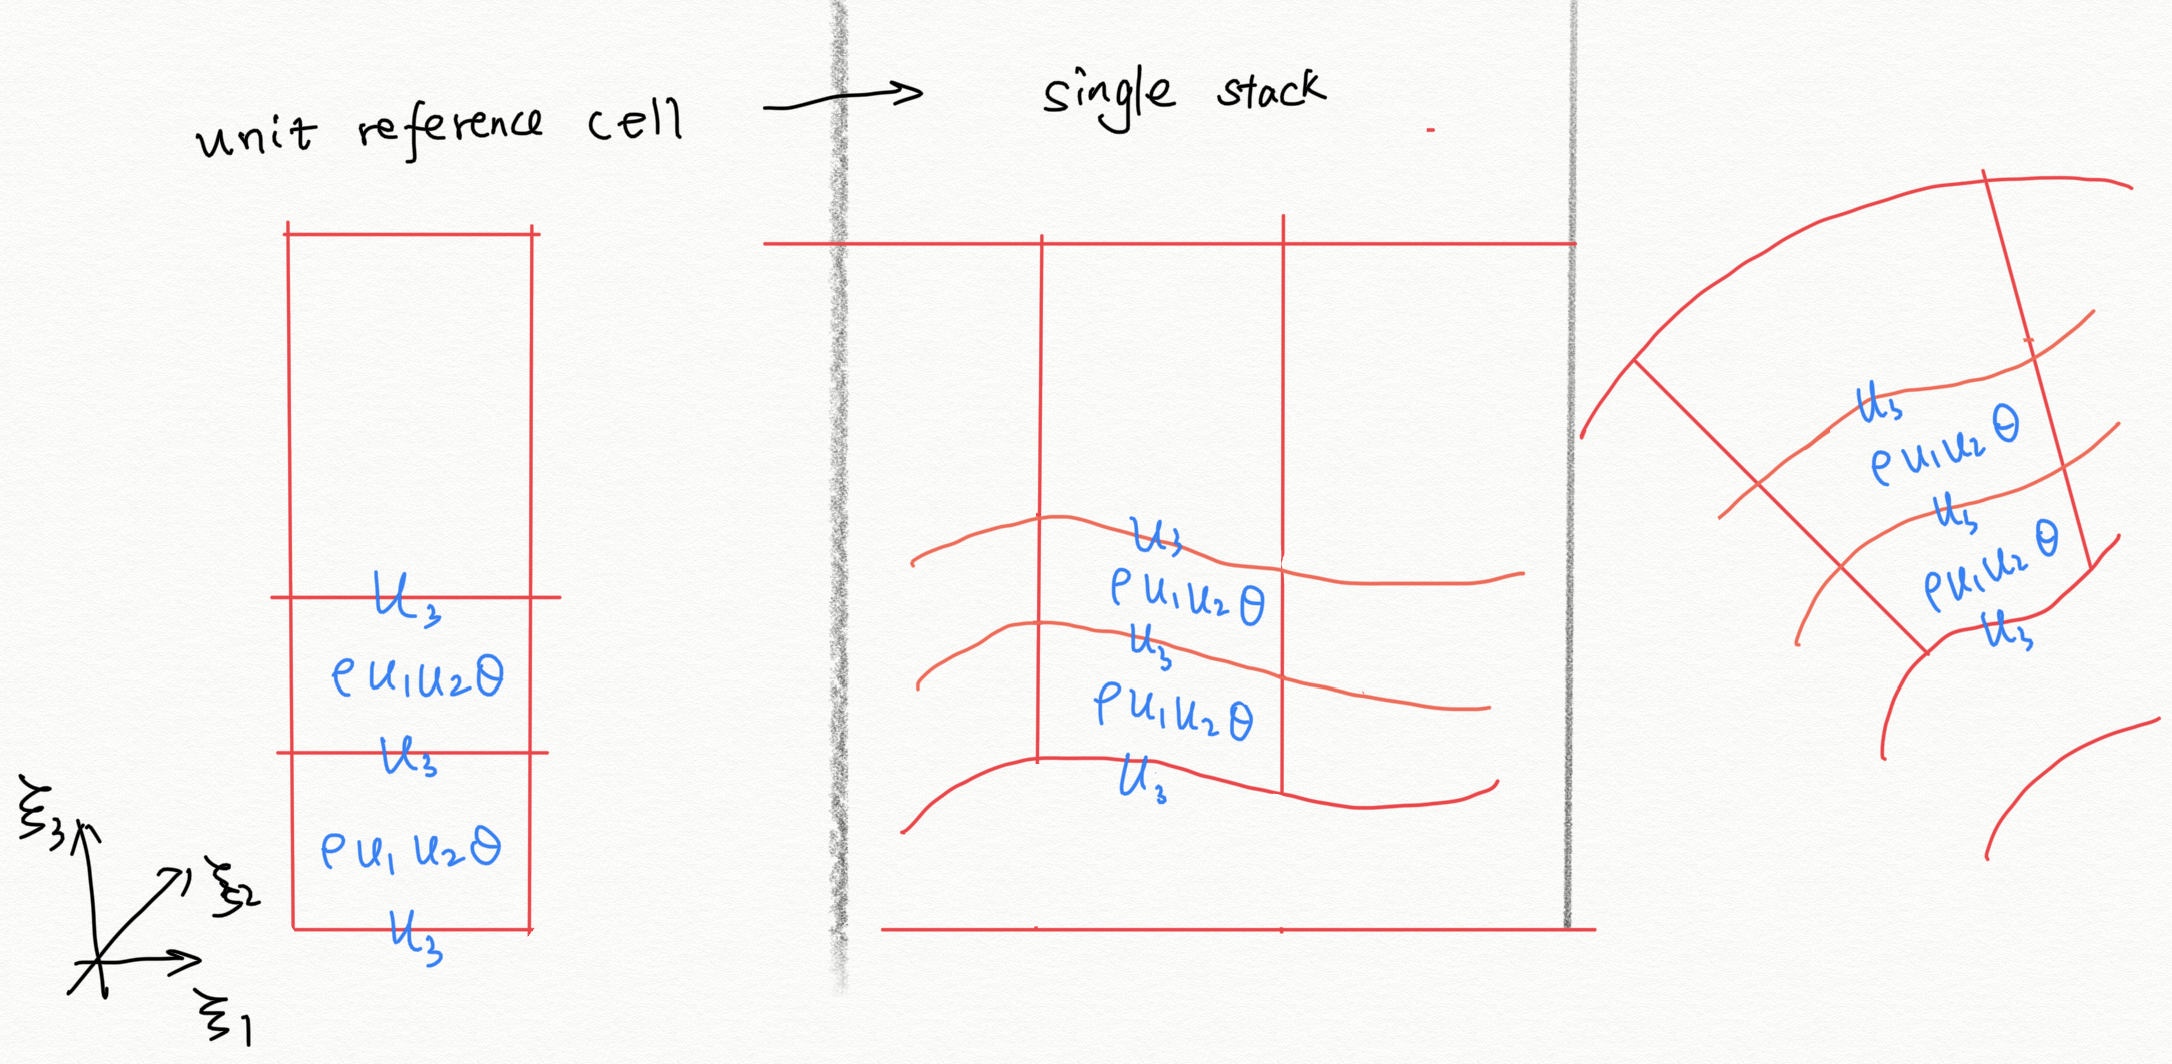
\includegraphics[width=0.8 \textwidth]{CLIMA-numerics/figures/staggered/StaggeredGrid.png}
    \caption{Schematics of staggered grid.}
    \label{fig:staggered-grid}
\end{figure}

Since we use terrain-follow coordinate system, the no penetration condition $\vec{u} \cdot \vec{n} = 0$ leads $u_3 = 0$ and $u^3 = 0$.

At each time step, we need to interpolate $u_3$ at cell centers, and interpolate  $\rho$, $u_j (j = 1,2)$, $\theta$, $J$, $g_{ij}$ \hl{do we need to interpolate metric terms} at cell faces (except top and bottom boundaries). And then compute $u^j$ at both cell centers and faces (except top and bottom boundaries). \hl{not sure should we interpolate $u^j$?}

The vertical derivative $\frac{\partial}{\partial\xi^3}$ is computed by the finite different method, as following
\begin{align*}
    \frac{\partial Q(\xi^3_{l})}{\partial\xi^3} \approx \frac{Q(\xi^3_{l+\frac{1}{2}}) - Q(\xi^3_{l-\frac{1}{2}})}{\xi^3_{l+\frac{1}{2}} - \xi^3_{l-\frac{1}{2}}}\\
    \frac{\partial Q(\xi^3_{l+\frac{1}{2}})}{\partial\xi^3} \approx \frac{Q(\xi^3_{l+1}) - Q(\xi^3_{l})}{\xi^3_{l+1} - \xi^3_{l}}\\
\end{align*}

The horizontal derivatives $\frac{\partial}{\partial\xi^1}$ $\frac{\partial}{\partial\xi^2}$ are computed by continuous Galerkin in the weak form  with 2D test functions \hl{not sure}.

Quantities involving first order derivatives, like $\Omega^k$, $\omega^k$, $\mathcal{T}^j$, at cell centers, are computed by combining the CG horizontal gradient and the finite different vertical gradient.  The values at cell faces are interpolated from cell center values. \hl{not sure}


Since $\xi^3$ is the vertical direction ($\frac{\partial Q}{\partial \xi^3} = \frac{\partial Q}{\partial r} \frac{\partial r}{\partial \xi^3}$), we have 
\begin{align*}
    \frac{\partial p_{ref}}{\partial \xi^3} = -\rho_{ref} \frac{\partial \Phi}{\partial \xi^3}
\end{align*}
The vertical velocity equation becomes 
\begin{align*}
    \frac{\partial}{\partial t} u_3 + \epsilon_{3kl} (2\Omega^k + \omega^k) u^l 
    &=  -\frac{1}{\rho} \frac{\partial p}{\partial\xi^3} 
    + \frac{1}{\rho_{ref}}\frac{\partial p_{ref}}{\partial\xi^3} 
   -  \frac{\partial}{\partial \xi^3} (K)  \nonumber\\
    & \quad + \mathcal{S}'_{u, 3} - g_{3j} \frac{1}{\rho} \nabla_k (\rho \tau^{jk}) - \mathcal{S}_\rho u_3,
    \label{e:equations_coord_hor_vert:velocity}\\
\end{align*}
\hl{not sure how to handle horizontal gradient}



\section{Governing equations}
\subsection{Potential temperature density}
Consider the 1-D model problem with potential temperature density
\begin{align*}
&\frac{\partial \rho}{\partial t} = - \frac{\partial (\rho w)}{\partial z}  \\
&\frac{\partial w}{\partial t} = - \frac{ \Theta}{\rho}\frac{\partial  \Pi}{\partial z} - g , \qquad \Pi = c_p\left(\frac{R_d\Theta}{p_0}\right)^{R/c_v}\\
&\frac{\partial \Theta}{\partial t} = - \frac{\partial (\Theta w)}{\partial z}
\end{align*}
where $\rho$ denotes density, $w$ vertical momentum component and $\Theta$ potential temperature density.

\subsection{Total energy density}
Consider instead the 1-D model problem with total energy density in place of the potential temperature conservation equation
\begin{align*}
&\frac{\partial \rho}{\partial t} = - \frac{\partial (\rho w)}{\partial z}  \\
&\frac{\partial w}{\partial t} = - \frac{\partial  w^2/2}{\partial z} - \frac{1}{\rho}\frac{\partial p}{\partial z} - g \\
&\frac{\partial E}{\partial t} = - \frac{\partial (E + p)w}{\partial z},  \qquad E = \frac{\rho w^2}{2} + \frac{p}{\gamma-1} + \rho g z
\end{align*}
where $E$ denotes total energy density.

\hl{[JK: Shouldn't the energy equation be?]}
\begin{align*}
E = \frac{\rho w^2}{2} + \frac{p}{\gamma-1} + \rho g z
\end{align*}

\section{Staggered Grid}
\subsection{Potential temperature density}
In a Finite Difference formulation, we use a staggered grid with $N$ cells so that different variables are defined at different discrete locations. We use cell-interfaces (points in 1D, edges in 2D, and faces in 3D) for the vertical momentum component, $w$, and cell-centers for $\rho$ and $\Theta$ that are thus collocated together.
\begin{align*}
&w_{1/2},          w_{1+1/2},          \cdots w_{N+1/2} \\
&\rho_{1}, \rho_{2} \cdots \rho_{N} \\
&\Theta_{1}, \Theta_{2} \cdots \Theta_{N}
\end{align*}

\begin{align*}
&\frac{\partial \rho_{i}}{\partial t} = - \frac{ \rho_{i+1/2} w_{i+1/2} - \rho_{i-1/2} w_{i-1/2} }{\Delta z}  \qquad \rho_{i+1/2} = \frac{ \rho_{i+1} +  \rho_{i}}{2}\\
&\frac{\partial w_{i+1/2}}{\partial t} = - \frac{1}{2}\left(\frac{ \Theta_{i+1}}{\rho_{i+1}} + \frac{ \Theta_{i}}{\rho_{i}}\right)\frac{ \Pi_{i+1}- \Pi_{i}}{\Delta z} - g \\
&\frac{\partial \Theta_{i}}{\partial t} = - \frac{\Theta _{i+1/2} w_{i+1/2} -  \Theta _{i-1/2} w_{i-1/2}   }{\Delta z} \qquad \Theta _{i+1/2} = \frac{\Theta _{i+1} + \Theta _{i}}{2}
\end{align*}

To obtain discrete hydrostatic balance, we require
\begin{align*}
   &\left(\frac{ \Theta_{i+1}}{\rho_{i+1}} + \frac{ \Theta_{i}}{\rho_{i}}\right)\frac{ \Pi_{i+1}- \Pi_{i}}{\Delta z}  = -2g \\
   & \rho_{i+1} = \frac{\Theta_{i+1}}{- \frac{2\Delta z g}{ \Pi_{i+1}- \Pi_{i} } -  \frac{ \Theta_{i}}{\rho_{i}}}
\end{align*}

\begin{figure}
    \centering
    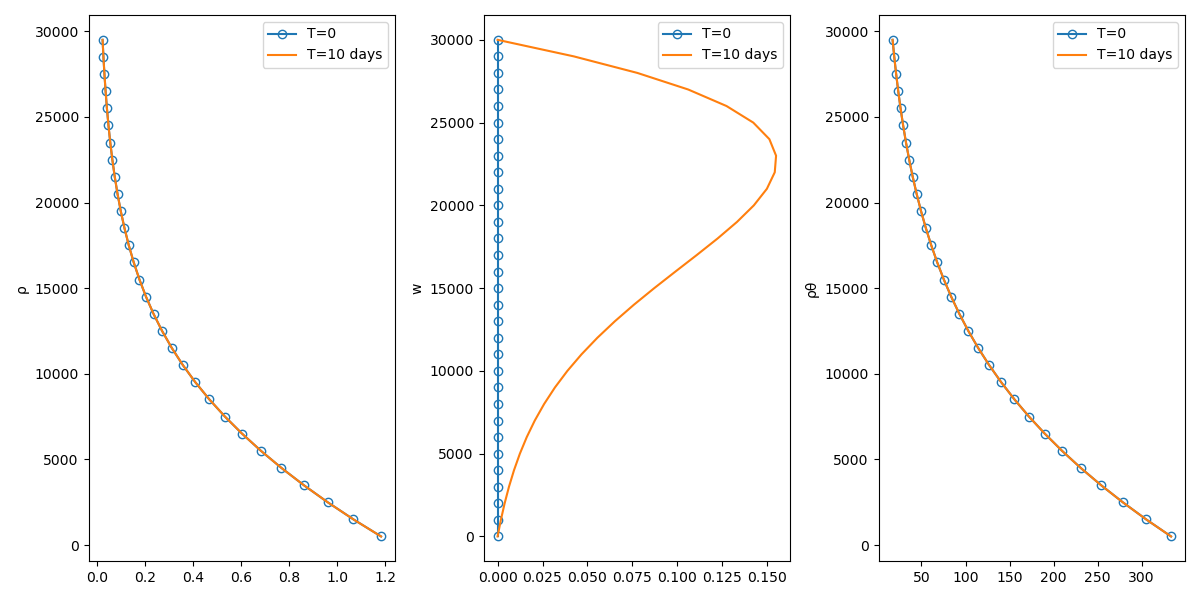
\includegraphics[width=0.45 \textwidth]{CLIMA-numerics/figures/staggered/HB-Theta-10-HB-false.png}
    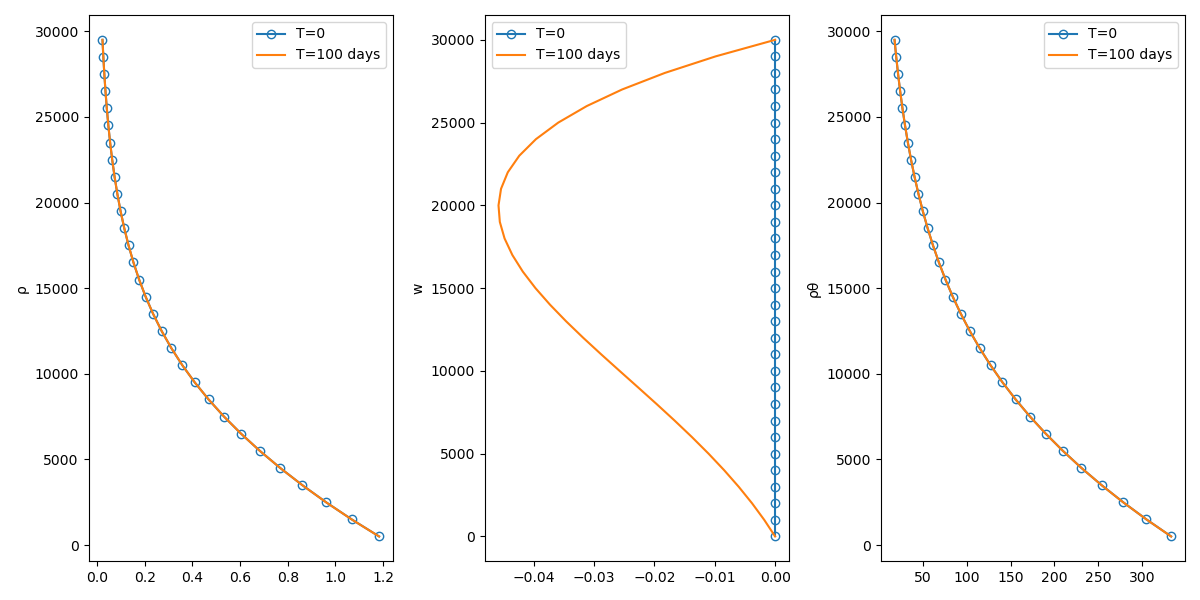
\includegraphics[width=0.45 \textwidth]{CLIMA-numerics/figures/staggered/HB-Theta-100-HB-false.png}
    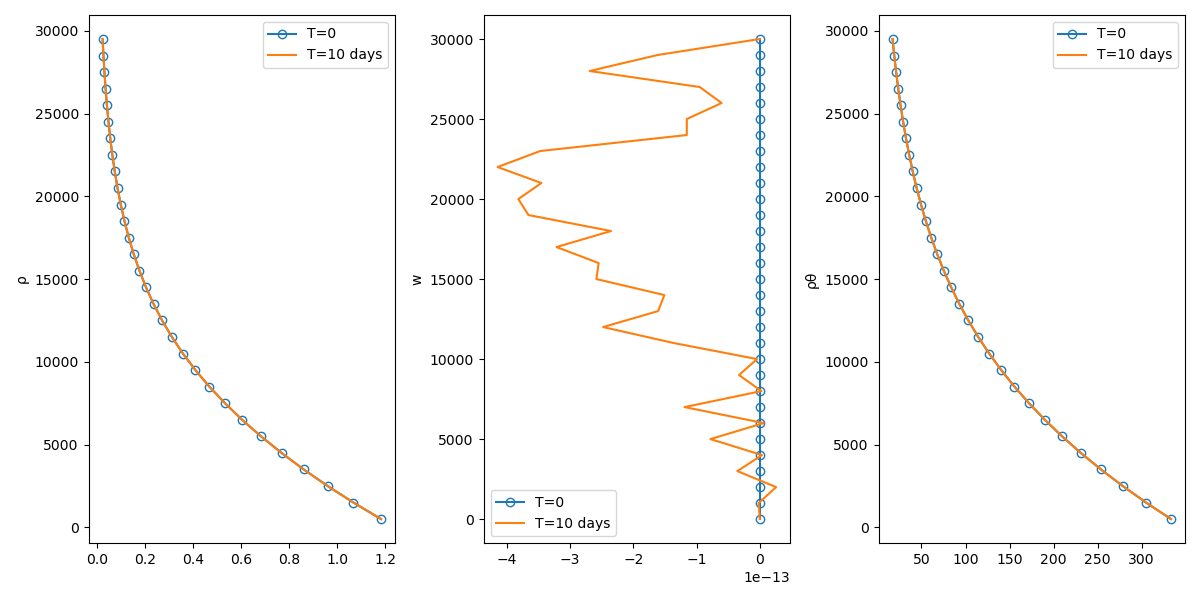
\includegraphics[width=0.45 \textwidth]{CLIMA-numerics/figures/staggered/HB-Theta-10-HB-true.png}
    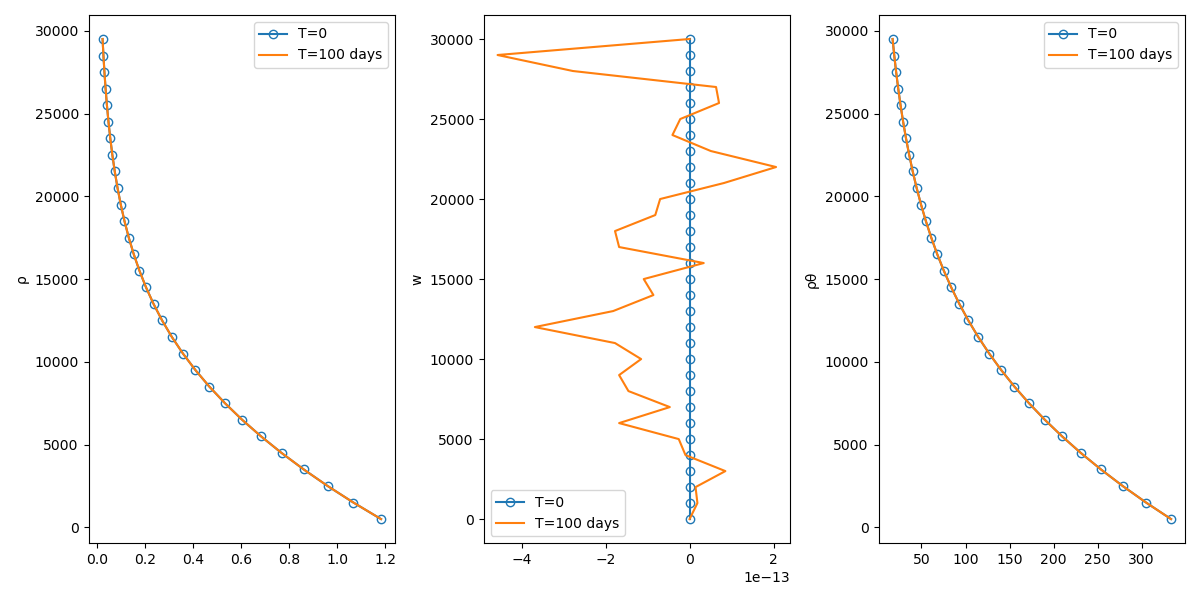
\includegraphics[width=0.45 \textwidth]{CLIMA-numerics/figures/staggered/HB-Theta-100-HB-true.png}
    \caption{Single column decaying temperature profile simulation with potential temperature density on staggered grid without discrete hydrostatic initialization (top)/with discrete hydrostatic initialization (bottom) for 10 days (left) and 100 days (right). Explicit RK4 with CFL=1.}
    \label{fig:my_label}
\end{figure}



\subsection{Total energy density}
Again, in a Finite Difference formulation, we use a staggered grid with $N$ cells so that different variables are defined at different discrete locations. We use a staggered grid with $N$ cells and use cell-interfaces (points in 1D, edges in 2D, and faces in 3D) for the vertical momentum component, $w$, and cell-centers for $\rho$ and $E$ that are thus collocated together.
\begin{align*}
&w_{1/2},          w_{1+1/2},          \cdots w_{N+1/2} \\
&\rho_{1}, \rho_{2} \cdots \rho_{N} \\
&E_{1}, E_{2} \cdots E_{N}
\end{align*}

\begin{align*}
&\frac{\partial \rho_{i}}{\partial t} = - \frac{ \rho_{i+1/2} w_{i+1/2} - \rho_{i-1/2} w_{i-1/2} }{\Delta z}\\
&\frac{\partial w_{i+1/2}}{\partial t} = -  \frac{ w_{i+3/2}^2 - w_{i-1/2}^2}{4\Delta z} - \frac{1}{2}\left(\frac{1}{\rho_{i+1}} +  \frac{1}{\rho_{i}}\right)\frac{ p_{i+1} - p_{i}}{\Delta z}  - g  \\
&\frac{\partial E_{i}}{\partial t} = - \frac{(E_{i+1/2} + p_{i+1/2}) w_{i+1/2} -  (E_{i-1/2} + p_{i-1/2}) w_{i-1/2}   }{\Delta z} \\
&p_{i+1/2} = (\gamma-1)\left( E_{i+1/2} - \frac{\rho_{i+1/2} w_{i+1/2}^2}{2} - \rho_{i+1/2} g z_{i+1/2} \right)
\quad E_{i+1/2} = \frac{E_{i+1} + E_{i}}{2} 
\quad \rho_{i+1/2} = \frac{\rho_{i+1} + \rho_{i}}{2} \\
&p_{i} = (\gamma-1)\left( E_{i} - \frac{\rho_{i} w_{i}^2}{2} - \rho_{i} g z_{i}\right) \quad w_{i} = \frac{w_{i+1/2} + w_{i-1/2}}{2}
\end{align*}



To obtain discrete hydrostatic balance, we require
\begin{align*}
   &\frac{1}{2}\left(\frac{1}{\rho_{i+1}} +  \frac{1}{\rho_{i}}\right)\frac{ p_{i+1} - p_{i}}{\Delta z}  = -g \\
   &E_{i+1}  = \frac{\frac{-2g}{\frac{1}{\rho_{i+1}} + \frac{1}{\rho_i}}\Delta z + p_i}{\gamma - 1} + \frac{\rho_{i+1}w_{i+1}^2}{2} + \rho_{i+1} g z_{i+1}
\end{align*}


\begin{figure}
    \centering
    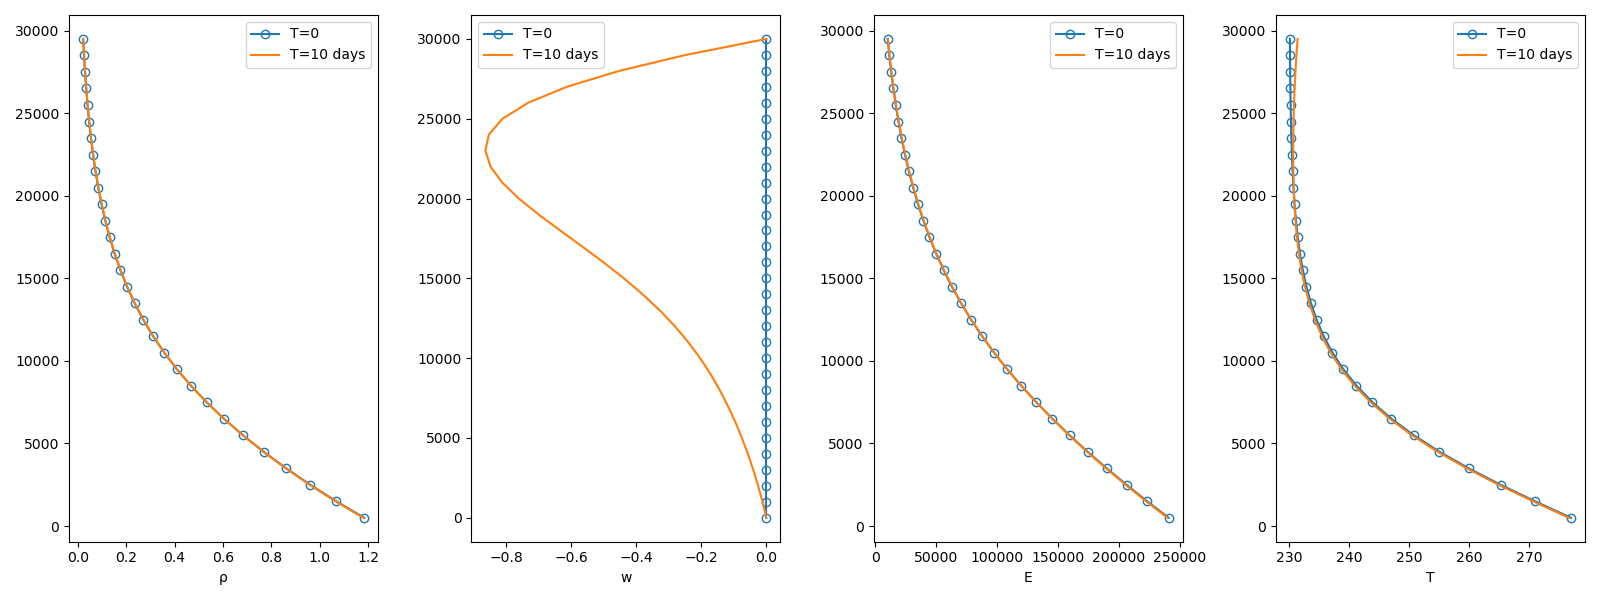
\includegraphics[width=0.45 \textwidth]{CLIMA-numerics/figures/staggered/HB-E-10-HB-false.png}
    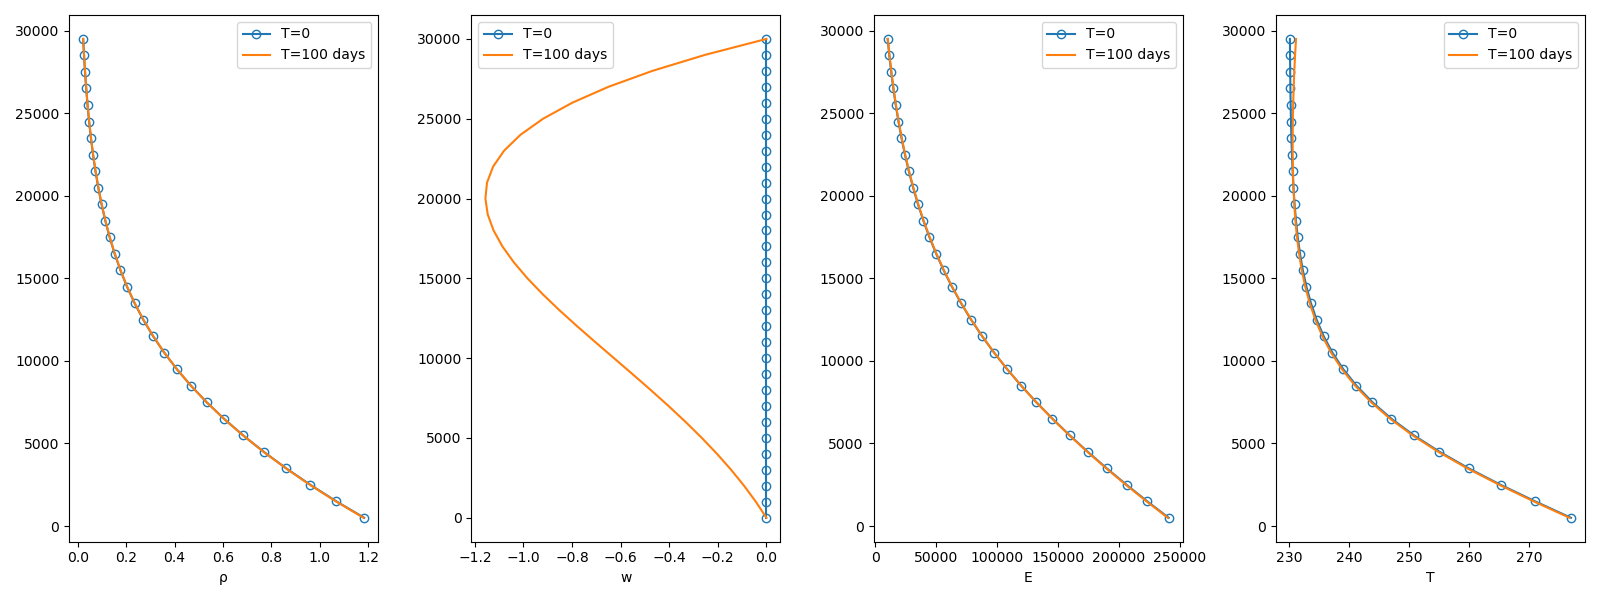
\includegraphics[width=0.45 \textwidth]{CLIMA-numerics/figures/staggered/HB-E-100-HB-false.png}
    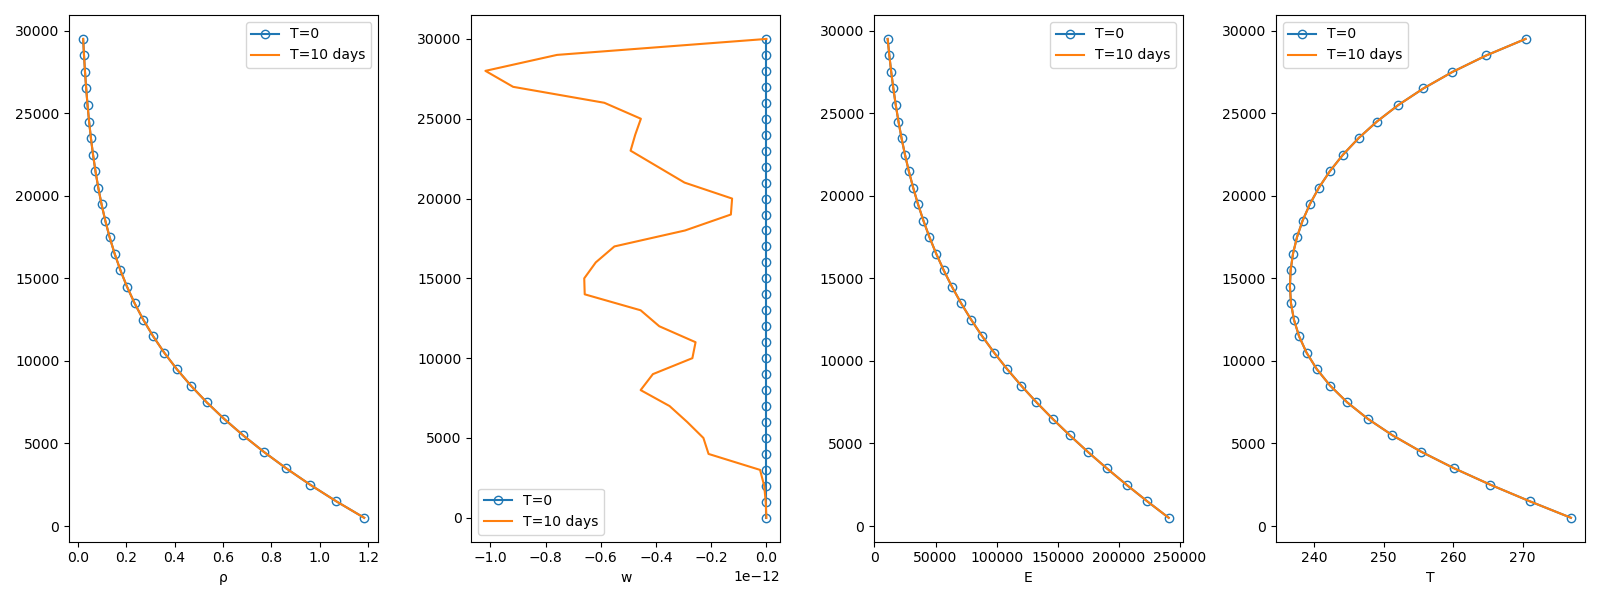
\includegraphics[width=0.45 \textwidth]{CLIMA-numerics/figures/staggered/HB-E-10-HB-true.png}
    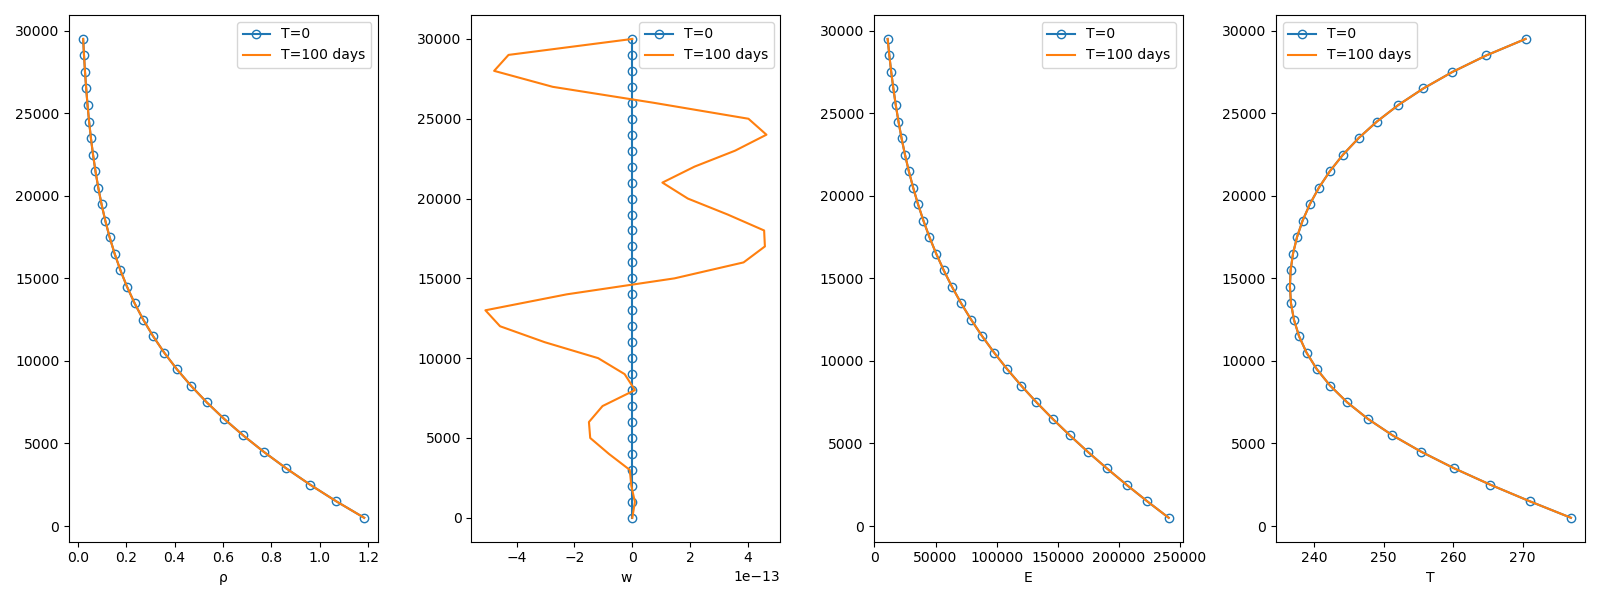
\includegraphics[width=0.45 \textwidth]{CLIMA-numerics/figures/staggered/HB-E-100-HB-true.png}
    \caption{Single column decaying temperature profile simulation with total energy density on staggered grid without discrete hydrostatic initialization (top)/with discrete hydrostatic initialization (bottom) for 10 days (left) and 100 days (right). Explicit RK4 with CFL=1.}
    \label{fig:my_label}
\end{figure}

Using energy as prognostic variable introduces larger error (without discrete hydrostatic balance treatment). And its discrete hydrostatic balance treatment is not straightforward. Simply updating $E_i$, which introduces errors, leads to weird temperature profile.

\subsection{With source term}
An artificial momentum source term $10\sin(\frac{2\pi t}{3600})$ is added at the second bottom layer, wave is generated 


\begin{figure}
    \centering
    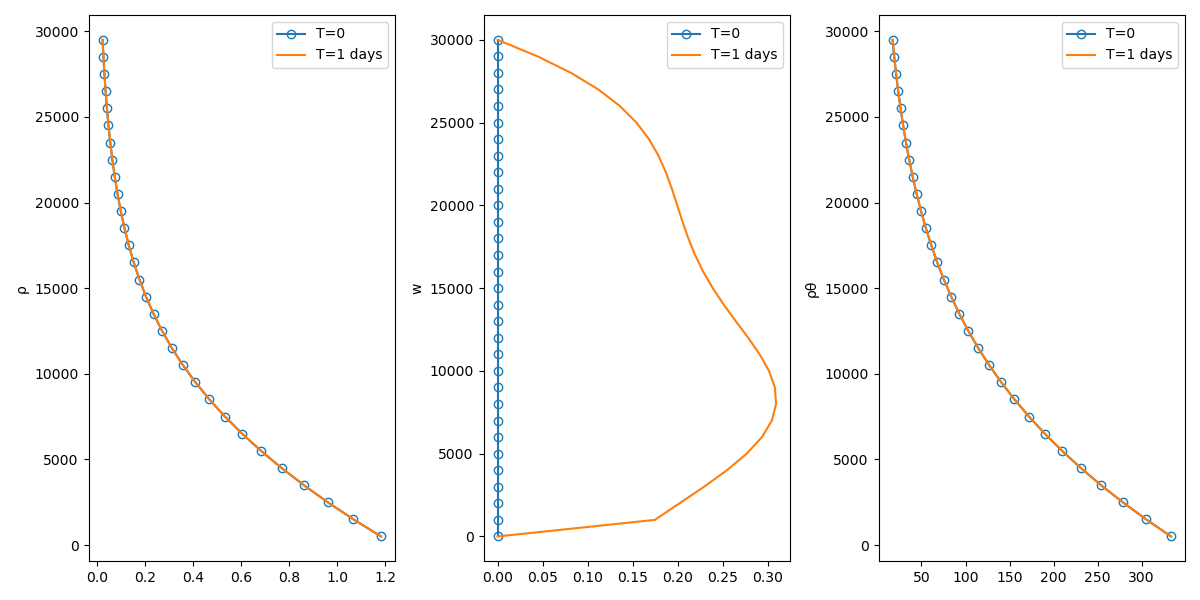
\includegraphics[width=0.45 \textwidth]{CLIMA-numerics/figures/staggered/wave-Theta-1-HB-true.png}\\
    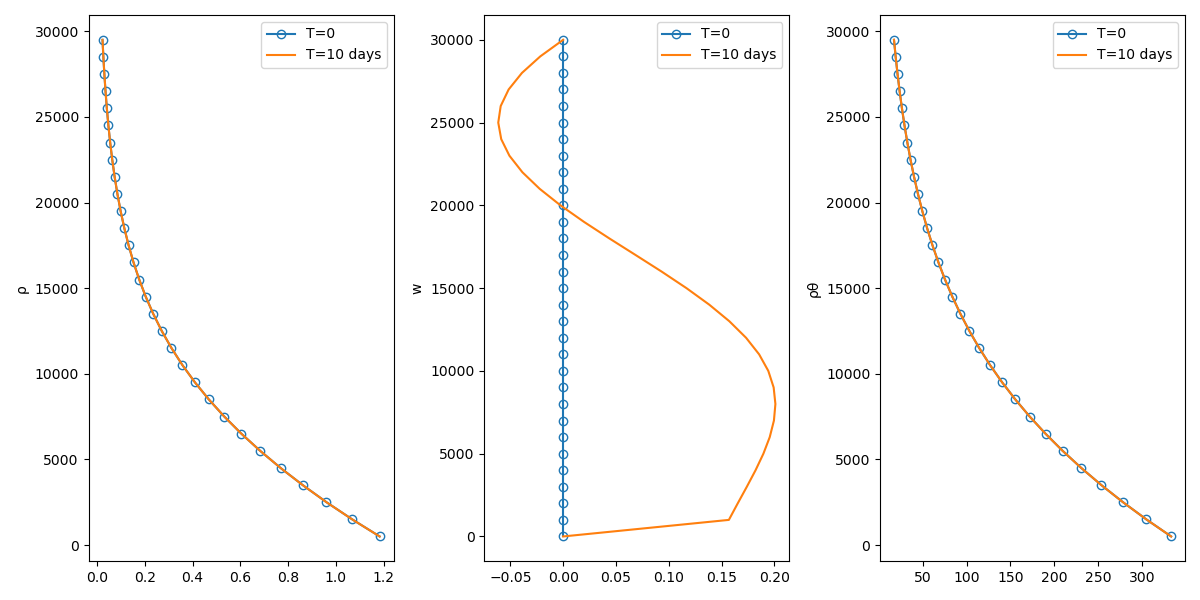
\includegraphics[width=0.45 \textwidth]{CLIMA-numerics/figures/staggered/wave-Theta-10-HB-true.png}\\
    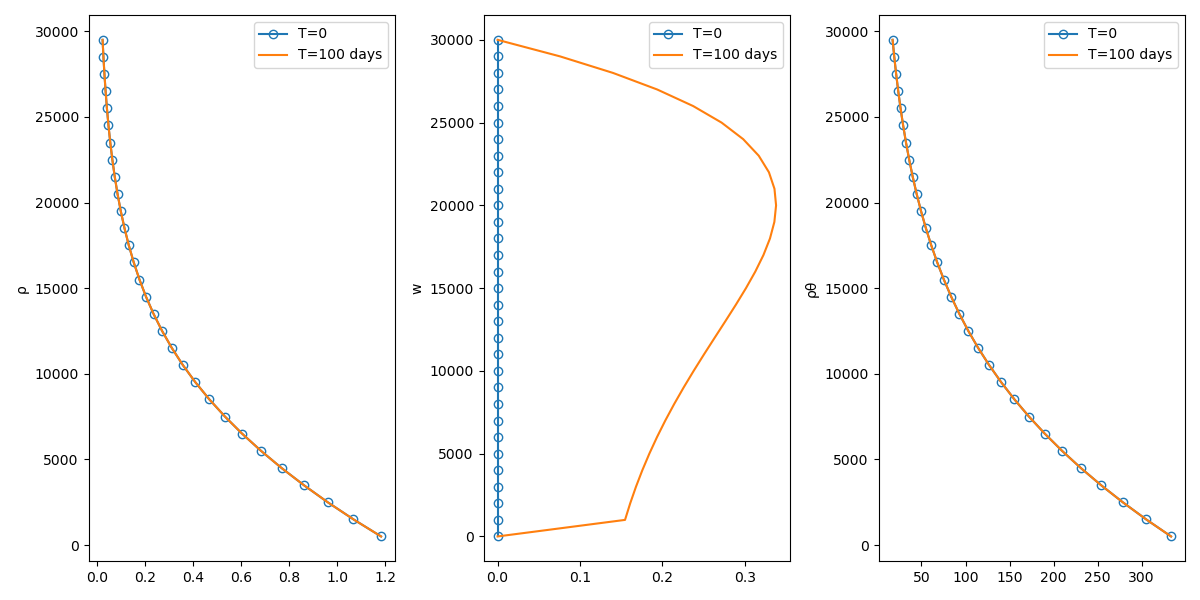
\includegraphics[width=0.45 \textwidth]{CLIMA-numerics/figures/staggered/wave-Theta-100-HB-true.png}
    \caption{Single column decaying temperature profile simulation with potential tempearature density on staggered grid with discrete hydrostatic initialization and a momentum source term for 1/10/100 days (top-to-bottom). Explicit RK4 with CFL=1.}
    \label{fig:my_label}
\end{figure}


\chapter{Spectral Element Discretization}

We discretize equations such as the balance laws in flux form \eqref{e:balance_equations_coord} or the equations in advective form \eqref{e:advective_equations_coord} using spectral elements in the generalized coordinates $(\xi^1, \xi^2, \xi^3)$. We assume the generalized horizontal coordinates parameterize a reference element of a spectral element discretization and are nondimensionalized such that $\xi^{i} \in [-1, 1]$, with $\xi^1$ and $\xi^2$ parameterizing the horizontal and $\xi^3$ the vertical. We require the discretization to have flexibility in the vertical so that different polynomial orders can be chosen for different variables (e.g., horizontal and vertical velocity components), so as to mimic the numerically beneficial effects of staggered grids \citep{Ullrich15c,Guerra16a}.

\hl{[describe CG implementation; horizontal as in CAM-SE/HOMME, following Taylor and Fournier and subsequent papers]}

We define the volume integrals for element $e = {[-1, 1]}^{d}$ as
\begin{align}
    \inner{\phi}{f}_{e} = \int_{e} \phi f,
\end{align}
and surface integrals
\begin{align}
    \inner{\phi}{f}_{\partial e} = \int_{\partial e} \phi f.
\end{align}
Volume and surface Jacobian determinants are added directly into expressions below.

The variational formulation for density \eqref{e:equations_coord_hor_vert:density} on the element $e$ is:
%\begin{subequations}
\begin{align}
   \inner{\phi}{\frac{\partial \rho J}{\partial t}}_{e}
   -
   \inner{\frac{\partial \phi}{\partial \xi^j}}
   {\rho J u^j}_{e}
    =&\; \inner{\phi}{J\rho \mathcal{S}_\rho}_{e} 
    - \inner{\phi}{J_{S} {\left(\rho u^j n_j\right)}^*}_{\partial e}.
\end{align}
The starred boundary integral indicates that, for the case of CG, only appears at the boundary whereas it contains a numerical flux if DG is used.
The term $J_{S}$ is the surface Jacobian which arises from the surface integral transformation.
Since we are tensor product in the reference space, on faces $\xi^{i}=\pm 1$ this will be
$J_{S} = |\vec{b}_{i+1} \times \vec{b}_{i+2}|$ (summation defined cyclically).
The unit normal is defined such that $J_{S} \vec{n} = \pm \vec{b}_{i+1} \times \vec{b}_{i+2}$
for faces $\xi^{i} = \pm 1$.

In the same way, the general tracer, $\theta$, \eqref{e:equations_coord_hor_vert:theta} is approximated as:
\begin{align}
   \inner{\phi}{\frac{\partial \rho \theta J}{\partial t}}_{e}&
   -
   \inner{\frac{\partial \phi}{\partial \xi^j}}
   {\rho \theta J u^j + \mathcal{T}^{j}}_{e}\nonumber\\
    &= \inner{\phi}{J\rho \mathcal{S}_\theta}_{e}
    - \inner{\phi}{J_{S}{\left(\left(\rho u^j + \mathcal{T}^{j}\right)n_{j}\right)}^*}_{\partial e}.
\end{align}
where $\mathcal{T}^j$ is computed within each element and is not DSSed (although possible terms appearing in the definition of $\mathcal{T}^j$ such as the diffusion coefficient may be DSSed to improve stability). For example:
\begin{align}
    \mathcal{T}^j = -D_t^{ji}\frac{\partial \hat{\xi}^k}{\partial \xi^i}\frac{\partial \theta}{\partial \hat{\xi}^k}
\end{align}
where $D_t^{ji}$ may or may not be DSSed.

For the velocity \eqref{e:equations_coord_hor_vert:velocity}, it is useful to consider
\begin{align}
  \int_{e} &\phi^{i}\frac{Jg_{ij}}{\rho} \nabla_{k}\left(\rho \tau^{jk}\right)\nonumber\\
  &=
  \int_{e} \phi^{i}\frac{g_{ij}}{\rho}\left[
  \frac{\partial}{\partial \xi^{k}}\left(J\rho\tau^{jk}\right)
  +
  J \rho \Gamma_{kl}^{j} \tau^{kl}
  \right]\nonumber\\
  &=
  \int_{e} \left[-
  J\rho\tau^{jk}
  \frac{\partial}{\partial \xi^{k}}\left(
  \frac{g_{ij}}{\rho}
  \phi^{i}
  \right)
  +
  Jg_{ij}\phi^{i} \Gamma_{kl}^{j} \tau^{kl}
  \right]
  +
  \int_{\partial e }
  \phi^{i} J_{S} {\left(\tau^{jk} g_{ij}n_{k}\right)}^{*}
  \nonumber\\
  &=
  -\inner{
  \frac{\partial}{\partial \xi^{k}}\left(
  \frac{g_{ij}}{\rho}
  \phi^{i}
  \right)
  }{
  J\rho\tau^{jk}
  }_{e}
  +
  \inner{\phi^{i}}{Jg_{ij} \Gamma_{kl}^{j} \tau^{kl}}_{e}
  +
  \inner{\phi^{i}}{J_{S} {\left(\tau^{jk} g_{ij}n_{k}\right)}^{*}}_{\partial e}
\end{align}
\hl{[JK] Is this correct? Idea is to try to move the derivative to the test function because ${\boldsymbol \tau}$ will involve derivatives.
I sort expected to get a $\nabla \vec{\phi}$ type term with just a boundary term, but I am not seeing it.} \hl{[TS] I think the way to discretize this is as in a flux-form equation: That is, you discretize the derivative, then divide nodal values pointwise by $\rho$ and multiply by $g_{ij}$. Here that amounts to not having $g_{ij}/\rho$ inside the integral but multiplying by this factor after discretization. Another $J$ factor should appear in the integral metric. --- But unfortunately, there is no way to write the whole thing as derivative plus boundary term, short of transforming velocities/stress tensor to Cartesian system (Vinokur 1974), because the Christoffel terms remain. The good news is that we will basically never need the Christoffel terms: We will only use fully 3d stress tensors in a box (LES), where the apparent sources from the coordinate transformation vanish; on a sphere, where they don't vanish, we will not use the fully 3d stress tensors, just hyperdiffusion, plus vertical diffusion, which can be written without Christoffel terms.}

The proposed velocity equation approximation is:
\begin{align}\label{e:var_equations_coord_hor_vert_mome}
    \inner{\phi^i}{J\frac{\partial  u_i}{\partial t}}_{e}&
    + \inner{\phi^i}{J\epsilon_{ikl}(2\Omega^k + \omega^k)}_{e}
    \nonumber\\
    =&
    -\inner{\phi^{i}}{\frac{J}{\rho}\frac{\partial p}{\partial \xi^k}}_{e}
    - \inner{\phi^i}{ J \frac{\partial}{\partial \xi^k} \left(\Phi + K \right)}_{e}
    \nonumber\\
    &
    +\inner{\phi^i }{J\left(S'_{u,i}-S_{\rho}u_i\right)}_{e}
    +\inner{
    \frac{\partial}{\partial \xi^{k}}\left(
    \frac{g_{ij}}{\rho}
    \phi^{i}
    \right)
    }{
    J\rho\tau^{jk}
    }_{e}
    \nonumber\\
    &
    -
    \inner{\phi^{i}}{Jg_{ij} \Gamma_{kl}^{j} \tau^{kl}}_{e}
    -
    \inner{\phi^{i}}{J_{S} {\left(\tau^{jk} g_{ij}n_{k}\right)}^{*}}_{\partial e}
    \nonumber\\
    &
    +
    \highlight{
    \inner{\phi^i}{J
    \left(
    g_{ij}u^{j}u^{k}n_{k}
    -
    {\left(g_{ij}u^{j}u^{k}n_{k}\right)}^{*}
    \right)}_{\partial e}
    }
    \end{align}
    where 
    \begin{align}
    \tau^{ij} &\propto 0.5 (g^{jk} \nabla_k u^i + g^{ik} \nabla_k u^j),\\
    \nabla_k u^i &= \frac{\partial u^i}{\partial \xi^k} + \Gamma_{kl}^i u^{l},\\
    \omega^{k} &= \frac{1}{J} \epsilon_{ijk} \frac{\partial u_{i}}{\partial \xi^{j}}.
\end{align}

Discretely, we approximate inner products with Legendre-Gauss–Lobatto (LGL) quadrature:
\begin{align}
    \inner{\phi}{\psi}_{e} &= \sum_{i,j=0}^{N_h}\sum_{k=0}^{N_v}w_{ijk}\phi_{ijk}\psi_{ijk}\\
    w_{ijk} &= w_i^h w_j^h w_k^v\\
    \phi_{ijk} &= \phi_i^h \phi_j^h \phi_k^v
\end{align}
where $N_h+1$ and $N_v+1$ are the number of LGL points in the horizontal and vertical directions, respectively.

\subsection*{Discrete Forms}

\hl{[JK] In the discrete forms below I do not have the boundary terms.
It's a bit unclear to me what's wanted, or how to do this in general, because
usually this is done for the equation as a whole, not the different operators.]}

Key discrete properties of LGL: let $(r_{[j]}, w_{[j]})$ for $j = 1, \dots, N_q$ be LGL quadrature points and weights.
We define the LGL derivative matrix $\mat{D}$ as
\begin{align}
    \mat{D}_{[i,j]} = l_{[i]}'(r_{[j]}),
\end{align}
where $l_{[i]}(x)$ is the Lagrange polynomial associated with LGL node $r_{[j]}$.
We also define the diagonal matrix of quadrature weights is $\mat{W}$
One of the key properties of LGL quadrature is that with $N_q = N + 1$ LGL nodes, we can exactly integrate polynomials of degree $2N - 1 = 2N_q -3$.
This means that though the integral of the product of two degree $N$ polynomials is not exact, we do have exact integration-by-parts
\begin{align}
    \dvec{\theta}^{T} \mat{W} \mat{D} \dvec{\sigma} =
    \int_{-1}^{1} \theta \sigma' =  
    {\left[\theta \sigma\right]}_{-1}^{1} - \int_{-1}^{1} \theta' \sigma' =
    \theta_{[N_q]} \sigma_{[N_q]} - \theta_{[1]} \sigma_{[1]} -  \dvec{\theta}^{T} \mat{D}^{T} \mat{W} \dvec{\sigma}.
\end{align}
Here $\dvec{\sigma}$ and $\dvec{\theta}$ are the vector of values at the LGL grid points.
this is often referred to as the summation-by-parts property and written as
\begin{align}
    \dvec{\theta}^{T} \mat{W} \mat{D} \dvec{\sigma} + \dvec{\theta}^{T} \mat{D}^{T} \mat{W} \dvec{\sigma}
    =  \theta_{[N]} \sigma_{[N]} - \theta_{[0]} \sigma_{[0]}
    =
    \dvec{\theta}^{T} \dvec{e}_{[N]} \dvec{e}_{[N]}^{T} \dvec{\sigma}
    -
    \dvec{\theta}^{T} \dvec{e}_{[0]} \dvec{e}_{[0]}^{T} \dvec{\sigma}
\end{align}
where $\dvec{e}_{[0]}$ and $\dvec{e}_{[N]}$ are the canonical unit basis vectors associated with the first and last grid points.

In multiple dimensions, we do not have exact integration by parts, but we do have a discrete equivalent:
\begin{align}
   \dvec{\theta}^{T} \mat{W} \mat{D}_{\xi^i} \dvec{\sigma} + \dvec{\theta}^{T} \mat{D}_{\xi^i}^{T} \mat{W} \dvec{\sigma}
   =
   \dvec{\theta}_{[\xi^i=-1]}^{T} \mat{W}_{i} \dvec{\sigma}_{[\xi^i=-1]}
   -
   \dvec{\theta}_{[\xi^i=1]}^{T} \mat{W}_{i} \dvec{\sigma}_{[\xi^i=1]}
\end{align}
where $\mat{D}_{\xi^i}$ is the tensor product derivative in the $\xi^{i}$ direction
and $\mat{W}_{i}$ is the mass matrix for surface integrals that along faces $\xi^{i} = \pm 1$,
and
$\dvec{\theta}_{[i=\pm1]}$ is the solution restricted to the face $\xi^{i} = \pm 1$.
Not that the LGL quadrature approximation is not exact for the surface integrals.

Assuming that in multiple dimensions that vectors are ordered with fastest index first,
\begin{align}
   \dvec{\sigma} =
   \begin{bmatrix}
   \sigma_{[1,1,1]}\\
   \sigma_{[2,1,1]}\\
   \vdots\\
   \sigma_{[N_q, 1, 1]}\\
   \sigma_{[1, 2, 2]}\\
   \vdots\\
   \sigma_{[N_q, N_q, N_q]}
   \end{bmatrix},
\end{align}
the tensor product form of the differentiation matrices are
\begin{align}
    \mat{D}_{\xi^1} = \mat{I} \otimes \mat{I} \otimes \mat{D},\\
    \mat{D}_{\xi^2} = \mat{I} \otimes \mat{D} \otimes \mat{I},\\
    \mat{D}_{\xi^3} = \mat{D} \otimes \mat{I} \otimes \mat{I}.
\end{align}

\subsubsection*{Strong-form Gradient of a Scalar on an element}
To compute the covariant components $u_{i}$ as a strong-form gradient $\theta$ we use
\begin{align}
    \inner{\phi}{J u_{i}} =  \inner{\phi}{J \frac{\partial \theta}{\partial \xi^{i}}},
\end{align}
which discretely gives
\begin{align}
    \dvec{\phi}^{T} \mat{W} \mat{J} \dvec{u}_{i} =   \dvec{\phi}^{T} \mat{W} \mat{J} \mat{D}_{\xi^i} \dvec{\theta},
\end{align}
which solving for $\dvec{u}_{i}$ is
\begin{align}
    \dvec{u}_{i} = \mat{D}_{\xi^i} \dvec{\theta}.
\end{align}

\subsubsection*{Weak-form Divergence of a vector field on an element}
To compute $\theta$ as a weak-form divergence $\vec{u}$ represented with contravariant components $u^j$
\begin{align}
   \inner{\phi}{J \theta}
   =
   -\inner{\frac{\partial \phi}{\partial \xi^j}}{Ju^j},
\end{align}
which discretely is
\begin{align}
   \dvec{\phi}^{T} \mat{W} \mat{J} \dvec{\theta}
   =
   -\dvec{\phi}^{T} \mat{D}_{\xi^j}^{T} \mat{W} \mat{J} \dvec{u^{j}}
\end{align}
or solving for $\dvec{\theta}$ gives
\begin{align}
   \dvec{\theta}
   =
   -\mat{W}^{-1} \mat{J}^{-1} \mat{D}_{\xi^j}^{T} \mat{W} \mat{J} \dvec{u^{j}}
\end{align}

For a continuous field the weak and strong form divergences are equivalent after the gather-scatter,
but for a field that is discontinuous they are different.
Such a discontinuous field might result from the (element) gradient of a field such as those that are used
for diffusion (div-grad).

\subsubsection*{Strong-form Divergence of a vector field on an element}
Included for completeness, but I see no reason that we will need this.

To compute $\theta$ as a strong-form divergence $\vec{u}$ represented with contravariant components $u^j$
\begin{align}
   \inner{\phi}{J\theta}
   =
   \inner{\phi}{\frac{\partial Ju^j}{\partial \xi^j}}
\end{align}
which discretely is
\begin{align}
   \dvec{\phi}^{T} \mat{W} \mat{J} \dvec{\theta}
   =
   \dvec{\phi}^{T} \mat{W} \mat{D}_{\xi^j} \mat{J} \dvec{u^{j}}
\end{align}
or solving for $\dvec{\theta}$ gives
\begin{align}
   \dvec{\theta}
   =
   \mat{J}^{-1} \mat{D}_{\xi^j} \mat{J} \dvec{u^{j}}
\end{align}

\subsubsection*{Strong-form Curl of a vector field on an element}
To compute the contravariant components $\sigma^i$ of the curl of a vector field $\vec{u}$ in terms
of the covariant components $u_j$ it is most natural to use the strong form
\begin{equation}
   \inner{\phi}{J v^i} = \inner{\phi}{\epsilon^{ijk} \frac{\partial u_k}{\partial \xi^j}},
\end{equation}
which leads to the discrete forms
\begin{equation}
   \dvec{\phi}^{T} \mat{W} \mat{J} \dvec{v}^i = \epsilon^{ijk} \dvec{\phi}^{T} \mat{W} \mat{D}_{\xi^j} \dvec{u}_{k},
\end{equation}
or solving for $\dvec{v}^i$ this is
\begin{equation}
   \dvec{v}^i = \epsilon^{ijk} \mat{J}^{-1} \mat{D}_{\xi^j} \dvec{u}_{k}.
\end{equation}

\subsubsection*{Weak-form divergence of a tensor on an element}
To compute the contraviant component $u^{i}$ as the weak-form
divergence of the tensor $\mat{\tau}$  with contravariant
components $\tau^{ij}$
we use
\begin{align}
  \int_{e} &\phi_{i}J u^{i}\nonumber\\
  &=
  \int_{e} \phi_{i}J \nabla_{j}\left(\tau^{ij}\right)\nonumber\\
  &=
  \int_{e} \phi_{i}\left[
  \frac{\partial}{\partial \xi^{j}}\left(J\tau^{ij}\right)
  +
  J \Gamma_{jk}^{i} \tau^{jk}
  \right]\nonumber\\
  &=
  \int_{e} \left[-
  J \tau^{ij}
  \frac{\partial}{\partial \xi^{j}}\left(
  \phi_{i}
  \right)
  +
  J\phi_{i} \Gamma_{jk}^{i} \tau^{jk}
  \right]
  +
  \int_{\partial e }
  \phi_{i} J_{S} {\left(\tau^{ij} n_{j}\right)}^{*}
  \nonumber\\
  &=
  -\inner{
  \frac{\partial}{\partial \xi^{j}}\left(
  \phi_{i}
  \right)
  }{
  J \tau^{ij}
  }_{e}
  +
  \inner{\phi_{i}}{J \Gamma_{jk}^{i} \tau^{jk}}_{e}
  +
  \inner{\phi_{i}}{J_{S} {\left(\tau^{ij} n_{j}\right)}^{*}}_{\partial e}.
\end{align}
Dropping the boundary term we get the discretization
\begin{align}
  \dvec{\phi}_{i}^{T} \mat{W} \mat{J} \dvec{u}^{i}
  =
  -\dvec{\phi}_{i}^{T} \mat{D}_{\xi^j}^{T} \mat{W} \mat{J} \dvec{\tau}^{ij}
  +
  \dvec{\phi}_{i}^{T} \mat{W} \mat{J} \mat{\Gamma}^{i}_{jk} \dvec{\tau}^{jk}.
\end{align}
Since the test function $\phi^{i}$ is arbitrary, we can solve for
$\dvec{u}^{i}$ to get
\begin{align}
  \dvec{u}^{i}
  =
  -\mat{W}^{-1} \mat{J}^{-1} \mat{D}_{\xi^j}^{T} \mat{W} \mat{J} \dvec{\tau}^{ij}
  +
  \mat{\Gamma}^{i}_{jk} \dvec{\tau}^{jk}.
\end{align}

Assuming that $\mat{\tau}$ comes from the gradient of a velocity field,
using the weak-form divergence is preferable to the strong form so that
symmetry of the operator results.

\subsubsection*{Strong-form divergence of a tensor on an element}
Included for completeness, to compute the contraviant component $u^{i}$ as
the strong-form divergence of the tensor $\mat{\tau}$  with contravariant
components $\tau^{ij}$ we use
\begin{align}
  \int_{e} &\phi_{i}J u^{i}
  =
  \int_{e} \phi_{i}J \nabla_{j}\left(\tau^{ij}\right)
  =
  \inner{
  \phi_{i}
  }{
  \frac{\partial}{\partial \xi^{j}}\left(
  J \tau^{ij}
  \right)
  }_{e}
  +
  \inner{\phi_{i}}{J \Gamma_{jk}^{i} \tau^{jk}}_{e}.
\end{align}
After discretization this becomes
\begin{align}
  \dvec{\phi}_{i}^{T} \mat{W} \mat{J} \dvec{u}^{i}
  =
  \dvec{\phi}_{i}^{T} \mat{W} \mat{D}_{\xi^j} \mat{J} \dvec{\tau}^{ij}
  +
  \dvec{\phi}_{i}^{T} \mat{W} \mat{J} \mat{\Gamma}^{i}_{jk} \dvec{\tau}^{jk},
\end{align}
and solving for $\dvec{u}^{i}$ we get
\begin{align}
  \dvec{u}^{i}
  =
  \mat{J}^{-1} \mat{D}_{\xi^j} \mat{J} \dvec{\tau}^{ij}
  +
  \mat{\Gamma}^{i}_{jk} \dvec{\tau}^{jk}.
\end{align}

\subsubsection*{Strong-form directional derivative of a scalar on an element}
To compute the scalar $\sigma$ as the directional derivative
$\vec{u} \cdot \nabla \theta$ of a scalar $\theta$ in the direction
vector $\vec{u}$ we compute
\begin{equation}
  \inner{\phi}{J \sigma} =
  \inner{\phi}{J u^j \frac{\partial\theta}{\partial \xi^j}}.
\end{equation}
Discretely this is
\begin{equation}
  \dvec{\phi}^{T} \mat{W} \mat{J} \dvec{\sigma}
  =
  \dvec{\phi}^{T} \mat{W} \mat{J}
  ~
  \mat{U}^j)
  ~
  \mat{D}_{\xi^{j}} \dvec{\theta},
\end{equation}
where $\mat{U}^j = \text{\tt Diagonal}(\vec{u}^{j})$.
After solving for $\dvec{\sigma}$ we have
\begin{equation}
  \dvec{\sigma}
  =
  \mat{U}^j \mat{D}_{\xi^{j}} \dvec{\theta}.
\end{equation}

\subsubsection*{Skew-form Scalar Diffusion on an element}

To compute the scalar $\beta$ which is the scalar diffusion of $\theta$
with diffusive tensor $\mat{T}$ we consider
\begin{equation}
  \inner{\phi}{J\beta}_{e}
  =
  \inner{\frac{\partial \phi}}{{\partial \xi^{i}}{J T^{ij} \frac{\partial\theta}{\partial \xi^j}}}_{e}.
\end{equation}
Discretely this is
\begin{equation}
  \dvec{\phi}^{T} \mat{W} \mat{J} \dvec{\beta}
  =
  \dvec{\phi}^{T} \mat{D}_{\xi^{i}} \mat{W} \mat{J} \mat{T}^{ij} \mat{D}_{\xi^{j}}\dvec{\theta},
\end{equation}
which upon solving for $\dvec{\beta}$ gives
\begin{equation}
  \dvec{\beta}
  =
  \mat{W}^{-1} \mat{J}^{-1} \mat{D}_{\xi^{i}} \mat{W} \mat{J} \mat{T}^{ij} \mat{D}_{\xi^{j}}\dvec{\theta},
\end{equation}

\subsubsection*{Skew-form Scalar Diffusion on an element}

\hl{[waiting on form to be written down]}

\subsubsection*{Gather-Scatter operation}
Once the element / discontinuous tendency is formed, we need to make it continuous.
This is essentially a discrete L2 projection operation from the discontinuous polynomial space
to the continuous polynomial space. For SEM, this can be achieved by a Jacobian determinant
weighted average of the ``duplicated'' nodes on the face.

Let $\sigma$ be a discontinuous piecewise polynomial field over the elements.
We are interested in defining a globally continuous piecewise polynomial solution $\theta$
such that
\begin{align}
  \int \phi J \theta = \int \phi J \sigma,
\end{align}
for all globally continuous piecewise polynomials $\phi$.
To do this discretely with SEM, it is natural to do it in a manner consistent with the LGL quadrature.
Namely we use an LGL approximation of each element for the integral approximation.

To do this, we let
$\bar{\dvec{\theta}}$ and $\bar{\dvec{\phi}}$
be the
global (unique node) CG field and test function. Additionally we define $\mat{Q}$ to be the scatter matrix
from the global CG to the element local (DG-storage) representation, thus the
solution $\sigma$ represented at the local / DG-storage nodes is
\begin{align}
    \label{eqn:DGCGProj}
    \dvec{\theta} = \mat{Q} \bar{\dvec{\theta}}.
\end{align}
Note that the matrix $\mat{Q}$ is only ones and zeros, with a row sum of $1$ and
column sum equal the the multiplicity of the nodes;
see \citet[page 192ff]{deville_fischer_mund_2002} for a discussion of $\mat{Q}$.

Let $\mat{W}_g = \mat{I}_{K} \otimes \mat{W}$ be the diagonal DG mass matrix
and $\mat{J}_{g}$ the diagonal global DG matrix of the Jacobian determinants.
With this the approximation of projection \eqref{eqn:DGCGProj} is
\begin{align}
   \bar{\dvec{\phi}}^{T} \mat{Q}^{T} \mat{W}_{g} \mat{J}_{g} \mat{Q} \bar{\dvec{\theta}}
   =
   \bar{\dvec{\phi}}^{T} \mat{Q}^{T} \mat{W}_{g} \mat{J}_{g} \dvec{\sigma}.
\end{align}
Solving for the desired CG solution vector we have that
\begin{align}
   \bar{\dvec{\theta}}
   =
   {\left(\mat{Q}^{T} \mat{W}_{g} \mat{J}_{g} \mat{Q}\right)}^{-1}
   \mat{Q}^{T} \mat{W}_{g} \mat{J}_{g} \dvec{\sigma}.
\end{align}
Typically we do not want to store $\bar{\dvec{\theta}}$ but instead the scattered solution
$\dvec{\theta}$, so we instead compute
\begin{align}
   \dvec{\theta}
   =
   \mat{Q} \bar{\dvec{\theta}}
   =
   \mat{Q} {\left(\mat{Q}^{T} \mat{W}_{g} \mat{J}_{g} \mat{Q}\right)}^{-1}
   \mat{Q}^{T} \mat{W}_{g} \mat{J}_{g} \dvec{\sigma}.
\end{align}
The matrix $\mat{Q}^{T} \mat{W}_{g} \mat{J}_{g} \mat{Q}$ is diagonal, and it can be shown that
\begin{align}
   \mat{Q} {\left(\mat{Q}^{T} \mat{W}_{g} \mat{J}_{g} \mat{Q}\right)}^{-1}
   = \text{\tt Diagonal}\left(\mat{Q} \mat{Q}^{T}
   \text{\tt diagm}\left(\mat{W}_{g}^{-1} \mat{J}_{g}^{-1}\right)\right) \mat{Q}.
\end{align}
Here the vector $\text{\tt diagm}\left(\mat{W}_{g}^{-1} \mat{J}_{g}^{-1}\right)$
is the inverse DG LGL weights and the Jacobian determinants at the nodal points. Using this we then have that
\begin{align}
   \dvec{\theta}
   =
   \text{\tt Diagonal}\left(\mat{Q} \mat{Q}^{T} \text{\tt diagm}\left(\mat{W}_{g}^{-1} \mat{J}_{g}^{-1}\right)\right) \mat{Q}\mat{Q}^{T} \mat{W}_{g} \mat{J}_{g} \dvec{\sigma}.
\end{align}
The matrix $\mat{Q} \mat{Q}^{T}$ is often called the direct stiffness summation (DSS),
but for efficiency it might be best for the whole operation with the mass matrices should be
implemented as a single kernel.

Note that to apply the projection operations to vectors which are stored as covariant and contravariant form,
the vectors components need to be expressed in the same
coordinate system. For example, with covariant velocities the the gather-scatter might be written as
\begin{align}
   \dvec{u}_{i}
   =
   \mat{T}_{ij}
   \mat{Q} {\left(\mat{Q}^{T} \mat{W}_{g} \mat{J}_{g} \mat{Q}\right)}^{-1}
   \mat{Q}^{T} \mat{W}_{g} \mat{J}_{g} \mat{R}_{jk}\dvec{v}_{k}.
\end{align}
where $\mat{R}_{jk}$ is the rotation from local to conforming coordinates and
$\mat{T}_{ij}$ is the rotation from conforming to local coordinates. With SEM the conforming
coordinate system need not be the global coordinate system, it could be one of the elements
as long as all shared nodes are rotated to the same coodinate frame.

\subsection*{Discrete Properties of Taylor and Fournier}

\subsubsection*{The discrete divergence theorem for periodic domains}

This follows directly from the SBP property of LGL and the fact that we are using weak
derivatives for divergence and strong derivatives for gradients (even with metric terms):
\begin{align}
   \inner{u^{i}}{J \frac{\partial f}{\partial^{i}}}_{e}
   &+
   \inner{\frac{\partial Ju^{i}}{\partial \xi^{i}}}{f}_{e}
   \approx
   {\left(\dvec{u}^{i}\right)}^{T} \mat{J} \mat{W} \mat{D}_{\xi^i} \dvec{f}
   +
   {\left(\dvec{u}^{i}\right)}^{T} \mat{J} \mat{D}^{T}_{i} \mat{W} \dvec{f}
   \nonumber\\
   &=
   \sum_{i=1}^{d} {\left[\mat{J}\dvec{u}^{i}\right]}_{i=-1}^{T} \mat{W}_{i} {\left[\dvec{f}\right]}_{i=-1}
   -
   \sum_{i=1}^{d} {\left[\mat{J}\dvec{u}^{i}\right]}_{i=1}^{T} \mat{W}_{i} {\left[\dvec{f}\right]}_{i=1}.
\end{align}
Since our element is aligned with the coordinate system $(\xi^{1}, \xi^{2}, \xi^{3})$
on face $\xi^{i} = \pm 1$ we will have that $J_{S} \vec{n} \cdot \vec{u} = \pm J \vec{u}^{i}$
where $J_{S}$ is the surface Jacobian and the $\vec{n}$ is the outward pointing normal to the face.
Thus if $\vec{J}_{S} \vec{n}$ and $\vec{u}$ are continuous across the face, then the (discrete)
surface integrals will vanish when summed over the whole (periodic) mesh.
Note that this assumes that the elements are conforming.

\subsubsection*{The discrete stokes}

TBD

\subsubsection*{Annihilator properties (WIP!)}

What we wish to show is that $\nabla \times \nabla f = \vec{0}$ and $\nabla \cdot \nabla \times \vec{u} = 0$.
Showing this is zero within an element is trivial because of the exactness of differentiation with LGL,
thus it is more interesting to show this holds when the intermediate quantities are DSSed.
Namely when approximating
\begin{align}
    \vec{v} &= \nabla f, \quad \nabla \times \vec{v} = \vec{u} = \vec{0}?,\\
    \vec{v} &= \nabla \times \vec{u}, \quad \nabla \cdot \vec{v} = f = 0?.
\end{align}
Let's consider the first equations, the CG discretization would be
\begin{align}
   \inner{\phi^{i}}{Jv_{i}}_{e} &= \inner{\phi^{i}}{J \frac{\partial f}{\partial \xi^{i}}}_{e}.\\
   \inner{\psi_{i}}{Ju^{i}}_{e} &= \inner{\psi_{i}}{\epsilon^{ijk} \frac{\partial v_{k}}{\partial \xi^{j}}}_{e},
\end{align}
where we $\phi^{i}$ and $\psi_{i}$ are the test functions and
$v_{i}$ and $u^{i}$ are the trial functions (all in continuous spaces).

\hl{[JK: Taylor-Fournier lacks details here, this will take more work\dots
need to consider DSS etc\dots
Also, Taylor-Fournier only considers 2-D and has restrictions on the mesh to certain connectivities
not sure if this means things don't work for more general meshes or just they didn't need it?]}

% \begin{subequations}
% \begin{align}
%  \frac{1}{J} \frac{\partial}{\partial t}  (\rho J) + \frac{1}{J} \frac{\partial}{\partial \xi^j} \left(\rho J u^j\right)
%    & = \rho \mathcal{S}_\rho,\\
%     \frac{\partial}{\partial t} u_i + \epsilon_{ikl} (2\Omega^k + \omega^k) u^l 
%     &=  -\frac{1}{\rho} \frac{\partial p}{\partial\xi^i} 
%    -  \frac{\partial}{\partial \xi^i} (\Phi + K)  \nonumber\\
%     & \quad + \mathcal{S}'_{u, i} - g_{ij} \frac{1}{\rho} \nabla_k (\rho \tau^{jk}) - \mathcal{S}_\rho u_i,\\
%         \frac{1}{J} \frac{\partial}{\partial t}  (\rho J \theta) + \frac{1}{J} \frac{\partial}{\partial \xi^j} \left(\rho J (u^j \theta + \mathcal{T}^j)\right)
%     & = \rho \mathcal{S}_\theta.
% \end{align}
% \end{subequations}


\section{Boundary Conditions}

\section{Filters}

All filters (spectral, SGS) need to act on conservable specific quantities, e.g., specific total enthalpy ($h_\mathrm{tot}$, \textbf{not} $\rho e$ etc.). To filter not conservable variables such as pressure and density, only filter fluctuations around hydrostatic reference state (locally computed, ideally).

On curved elements, filters need to conserve mass. This means that in addition to damping the highest modes, we also want the lowest mode to be the same before and after filtering.

\subsection{Hyperviscosity and Hyperdiffusion}

follow \citet{Dennis12a} and \citet{Guba14a} for CG implementation 

\subsection{Spectral Filters}

%%%%%%%%%%%%%%%%%%%%%%%%%%%%%%%%% Time Discretization Chapter %%%%%%%%%%%%%%%%%%%%%%%%%%%%%%%%%%%%%%%%
\chapter{Time Discretization}\label{s:timestepping}

For the atmosphere, the general, compressible equations of motion we use permit a variety of wave modes with different characteristic speeds. Additionally, the equations contain sources that can add stiffness, for example, microphysical processes that occur on timescales of seconds or less. Similarly, stiffness in the land model arises near where the soil reaches saturation and timescales become very short.

The atmosphere equations permit the following wave modes:
\begin{itemize}
    \item Acoustic waves. They have phase speeds around $300~\mathrm{m~s^{-1}}$ in the atmosphere. Density variations and the terms involving pressure in the momentum and energy equations are essential for their existence.
    \item Gravity waves. They have a spectrum of phase speeds. In a deep atmosphere (e.g., in a GCM), the gravest, external mode has phase speed $(gH)^{1/2} \approx 280~\mathrm{m~s^{-1}}$, where $H\approx 8~\mathrm{km}$ is the atmospheric scale height. The gravity term $-\rho \nabla \Phi$ in the momentum equation and the gravitational potential energy $\Phi$ in the energy equation are responsible for their existence.
    \item Inertia-gravity, Rossby waves, and several other wave modes that owe their existence to the Coriolis acceleration $-2\vec{\Omega} \times \rho \vec{u}$ in the momentum equation. They have smaller phase speeds than the acoustic and external gravity waves.
\end{itemize}
Additional stiffness in the equations arises from:
\begin{itemize}
    \item Falling precipitation, whose fall velocity $w_{p,i}$ can reach $10~\mathrm{m~s^{-1}}$ and thus exceeds typical vertical velocities resolved in GCMs.
    \item Microphysical source terms, for example, in the equations for suspended specific humidities $q_k$; they depend on the precipitation specific humidity $q_{p,i}$, which can change rapidly because precipitate falls rapidly. 
    \item SGS diffusive fluxes, whose effective vertical velocity can exceed that of the resolved velocities.
    \item Other parameterized SGS fluxes, for example, convective updrafts, whose vertical velocities can likewise be large.
\end{itemize}
By contrast, radiation evolves on longer timescales than the dynamical quantities and hence, because it is expensive to evaluate, usually is evolved forward in time with longer timesteps than the dynamical quantities. 

We need a stable and computationally efficient time discretization strategy that allows some state vector components to be treated implicitly (e.g., falling precipitation and convective updrafts) and allows other terms (e.g., radiative energy fluxes) to be evaluated less frequently than dynamical terms. In particular, we need a computationally efficient way of handling the physically insignificant acoustic waves.
     
\section{Decomposition of Time Tendencies}

To circumvent the time-step restriction due to the fast acoustic and gravity waves, using implicit-explicit (IMEX) methods is one option. For the LES model, if the aspect ratio of the horizontal ($\Delta_h$) to vertical ($\Delta_v$) grid spacing is near unity, using fully 3D-IMEX methods may be an option.  For LES models with aspect ratios of grid elements $\Delta_h/\Delta_v > 1$ and for global atmospheric models, which generally have $\Delta_h/\Delta_v \gg 1$, we use 1D-IMEX methods in which the time-integrator is fully explicit in the horizontal direction (HE) and implicit in the vertical direction (so-called HEVI schemes). 

IMEX methods require the solution of one or more linear systems at each time step. The linear system is global in 3D, and this may limit scalability of IMEX methods in a multi-node computational setting. In that case, explicit methods in the horizontal, potentially with subcycling of fast terms in a multirate setting, may be a more scalable option to deal with the timestep restrictions. For HEVI schemes, the linear solves are restricted to independent atmospheric columns, which are generally represented on a single compute node. So their scalability across nodes is less restricted.

All of these approaches are based on a decomposition of time tendencies $\Tvector$ into four terms: 
\begin{itemize}
    \item terms to be treated implicitly, labeled by $I$ (the fastest terms);
    \item terms evaluated at the dynamical (advective) timestep, labeled by $d$;
    \item terms to be subcycled $f$ times for each dynamical timestep, labeled by $+f$ (for fast);
    \item terms to be evaluated every $s$ dynamical timesteps, labeled by $-s$ (for slow).
\end{itemize}
With this, we can write the system of ODEs obtained by the space discretization symbolically as
\[
\frac{\partial \vec{Y}}{\partial t} = \Tvector  = \Tvector_{I} + \Tvector_{d} + \Tvector_{+f} + \Tvector_{-s},
\]
where $\vec{Y}$ is a vector of state variables of the model. 

To obtain a linear problem for linear implicit solves, let us linearize the implicit tendency terms $\Tvector_{I}$ by Taylor expansion around a reference state $\vec{Y}_r$,
\begin{equation}\label{e:imex_linearization}
\Tvector_{I}(\vec{Y}) =  \Tvector_I(\vec{Y}_r) + \vec{\mathcal{L}}_I (\vec{Y} - \vec{Y}_r) + \Tvector^N_{I}(\vec{Y}),
\end{equation}
where 
\begin{equation}
    \vec{\mathcal{L}}_I = \left. \frac{\partial\Tvector_I}{\partial\vec{Y}}\right|_{\vec{Y}_r}
\end{equation} 
is the linear component of the tendency operator and $\Tvector^N_{I}(\vec{Y})$ is the nonlinear residual. This then allows us to write the equation of motion \eqref{e:eom_compact} as
\begin{equation}
\label{e:IMEX}
\frac{\partial\vec{Y}}{\partial t} =  \vec{\mathcal{L}}_I \vec{Y} + \Bigl(\Tvector_I(\vec{Y}_r) - \vec{\mathcal{L}}_I \vec{Y}_r\Bigr) + \Tvector^N_{I}(\vec{Y}) + \Tvector_{d} + \Tvector_{+f} + \Tvector_{-s}.
\end{equation}
Usually, the reference state $\vec{Y}_r$ is chosen so that the tendency of the reference state, $\Tvector_I(\vec{Y}_r)$, and the linear tendency of the reference state, $\vec{\mathcal{L}}_I \vec{Y}_r$, either vanish individually or cancel each other, so that $\Tvector_I(\vec{Y}_r) - \vec{\mathcal{L}}_I \vec{Y}_r=0$. We will justify this in section~\ref{s:IMEX_general}.

\section{Reference State for Linearization}

Solving for the fastest waves implicitly by a linear solve requires linearization of the fastest tendency terms. We generally use reference states characterized by a temperature $T_r(z)$ that may depend on height $z$ but does not depend on horizontal coordinates or time. We enforce hydrostatic balance, and assume the reference state is dry.
%so that the reference state variables are obtained as described in section~\ref{s:initial_conditions} with zero relative humidity ($\mathrm{RH}=0$): the pressure is obtained from \eqref{e:hydro_pressure}, the density from \eqref{e:hydro_density}, and the total specific humidity is set to zero, $q_{t,r}=0$.

Because the reference temperature and thus the reference pressure are assumed to be constant in the horizontal, the reference state is assumed at rest, $\vec{u}_r = 0$, consistent with geostrophic balance. Because the reference state is assumed dry, $q_k= 0$ for $k \in \{ t, v, l, i, p\}$ in the reference state.

More sophisticated reference states for linearization are possible, for example, with a latitudinally varying hydrostatically balanced temperature profile, and with a reference velocity in geostrophic and hydrostatic balance with this temperature field. However, we focus on hydrostatic states at rest for now. 
 
 \section{Solving for Acoustic and Gravity Waves Implicitly}
 \label{s:IMEX_general}

Let us lay out in general terms the linearizations for acoustic and gravity waves that underlie IMEX methods in 1D and 3D. The tendency terms responsible for acoustic waves and gravity waves are
 \begin{equation}
 \Tvector_{I}= -\nabla_{1/3} \cdot
 \begin{pmatrix}
 \rho \vec{u} \\
 p \vec{I}_3 \\
 \bigl(e^{\mathrm{tot}} + (\delta_{\mathrm{gw}}-1) \Phi + p/\rho \bigr) \rho \vec{u} \\
 0\\
 \vdots
 \end{pmatrix}
 - \begin{pmatrix}
 0 \\
 \delta_{\mathrm{gw}} \rho \nabla_{1/3} \Phi \\
 0\\
 0\\
 \vdots
 \end{pmatrix},
 \label{e:3D-imex/tendencies}
 \end{equation}
where all components indicated by dots are zero. The operator $\nabla_{1/3}$ is the 3D differential operator $\nabla_3 = \nabla$ for 3D-IMEX, and it is the 1D operator $\nabla_1 = \vec{k} \partial/\partial_z$ for 1D-IMEX. (The geopotential gradient $\nabla_{1/3} \Phi$ only has a vertical component as long as we consider a spherical planet, so this gradient even in 3D usually only has a vertical component.) The switch $\delta_{\mathrm{gw}}$ (which can only take the value of either $0$ or $1$) is included to indicate whether gravity waves are included in the implicit tendencies: 
\begin{itemize}
    \item $\delta_{\mathrm{gw}}=1$: both acoustic and gravity waves are included in $\Tvector_I$;
    \item $\delta_{\mathrm{gw}}=0$: only acoustic waves are included in $\Tvector_I$.
\end{itemize}

In the tendency \eqref{e:3D-imex/tendencies}, the terms that need to be linearized are the pressure $p$, which depends nonlinearly on state variables, and the total enthalpy flux $(\rho e^{\mathrm{tot}} + p/\rho) (\rho \vec{u})$. Linearization around a state of rest ($\vec{u}_r=0$) with reference total energy $e^{\mathrm{tot}}_r$, pressure $p_r$, and density $\rho_r$ leads to
 \begin{equation}\label{e:IMEX_linear}
 \vec{\mathcal{L}}_I \vec{Y} = 
 -\nabla_{1/3} \cdot \begin{pmatrix}
 \textcolor{blue}{\rho \vec{u}} \\
 \textcolor{blue}{p_L} \vec{I}_3  \\
 \Bigl(e^{\mathrm{tot}}_r  + (\delta_{\mathrm{gw}}-1)\Phi + p_r/\rho_r \Bigr) \textcolor{blue}{\rho \vec{u}}\\
 0\\
\vdots
\end{pmatrix}
-
\begin{pmatrix}
0 \\
\delta_{\mathrm{gw}} \textcolor{blue} \rho \nabla_{1/3} \Phi \\
0\\
0\\
\vdots
\end{pmatrix}.
\end{equation}
This is linear with respect to \textcolor{blue}{$\rho$} and \textcolor{blue}{$\rho \vec{u}$} (all state variables and linear functions thereof are colored \textcolor{blue}{blue}; all other terms are constants or fixed functions of height $z$). For it to be a linear function of all state variables, the pressure \textcolor{blue}{$p_L$} needs to be expressed as a linear function of state variables. To derive a linear approximation for the pressure, we use the ideal gas law $p = R_m (\rho T)$ and the expression derived from the temperature equation 
%Eq.~\eqref{e:temperature} 
for $\rho T$ in terms of the internal energy and specific humidities,
\begin{equation}\label{e:pressure}
\begin{split}
p &= R_m (\rho T) \\
  &= \rho R_m T_0 + \frac{R_m}{c_{vm}} \left[\rho e^{\mathrm{tot}} - \rho \Phi - 0.5 \rho \|\vec{u}\|^2 - (\rho q_t - \rho q_l) I_{v,0} + \rho q_i (I_{i,0} + I_{v,0}) \right],
\end{split}
\end{equation}
where we have used the relation $I = e^{\mathrm{tot}} - \Phi - 0.5 \|\vec{u}\|^2$ between total and internal energy. Linearization $p_L = p_r + (\partial p/\partial\vec{Y})\cdot(\vec{Y}-\vec{Y}_r)$ around the reference state $\vec{Y}_r$ with pressure $p_r$ and zero specific humidities leads to 
\begin{equation}\label{e:pressure_linear}
\textcolor{blue}{p_L} = \textcolor{blue}{\rho} R_d T_0 + \frac{R_d}{c_{vd}} \bigl[ \textcolor{blue}{\rho e^{\mathrm{tot}}} - \textcolor{blue}{\rho} \Phi - (\textcolor{blue}{\rho q_t} - \textcolor{blue}{\rho q_l})I_{v,0} + (\textcolor{blue}{\rho q_i}) (I_{i,0} + I_{v,0}) \bigr].
\end{equation}
If only the total specific humidity $q_t$ is available as a prognostic variable and condensate is determined by saturation adjustment, the condensate specific humidities $q_l$ and $q_i$ in this linearized expression for the pressure can be set to zero. Note that the temperature $T_0$ that appears here is the \emph{reference temperature in the definition of internal energy}, a model constant; it is \emph{not} the temperature $T_r$ of the reference state about which we linearized. In fact, the linearized pressure \eqref{e:pressure_linear} does not depend on the reference state: the zeroth-order term $p_r$ in the linearization cancels the terms involving the reference state in the linear term, which ensures that the linearized pressure vanishes when the density vanishes. 

We can now see that the sum of the terms involving the reference state in the decomposition \eqref{e:imex_linearization} vanishes,
\[
\Tvector_I(\vec{Y}_r) - \vec{\mathcal{L}}_I \vec{Y}_r = 0.
\]
To see this, it is useful to distinguish the cases when gravity waves are included in the implicit term and when they are not included: 
\begin{itemize}
    \item Acoustic and gravity waves included ($\delta_{\mathrm{gw}}=1$). In this case, it is evident that $\Tvector_I(\vec{Y}_r)=0$ because the pressure gradient ($-\nabla_{1/3} p_r(z)$) and geopotential gradient ($-\rho_r\nabla_{1/3}\Phi$) in the momentum equation (second component of tendency vector) cancel for a hydrostatic reference state with $p_r = p_r(z)$. The same is true for the linear term for a reference state at rest, for which $p_L = p_r$ and $\vec{\mathcal{L}}_I \vec{Y}_r = 0$. 
    \item Only acoustic waves included ($\delta_{\mathrm{gw}}=0$). In this case, neither $\Tvector_I(\vec{Y}_r)$ nor $\vec{\mathcal{L}}_I\vec{Y}_r$ vanish individually, because the geopotential term needed for the cancellation of terms in hydrostatic balance does not appear in the momentum tendency. However, $p_L = p_r$ in a reference state at rest, so that $\Tvector_I(\vec{Y}_r) = \vec{\mathcal{L}}_I\vec{Y}_r$.
\end{itemize}
Thus, in either case, the terms involving the reference state do not appear  in the decomposition \eqref{e:imex_linearization}. 

The nonlinear term follows as the residual 
\begin{equation}\label{e:nonlinear_residual}
\begin{split}
\Tvector^N_{I}(\vec{Y}) & =  \Tvector_I(\vec{Y}) - \vec{\mathcal{L}}_I \vec{Y} \\
& = 
-\nabla_{1/3} \begin{pmatrix}
0 \\
(p - p_L) \vec{I}_3\\
(e^{\mathrm{tot}}  + p/\rho - e^{\mathrm{tot}}_r - p_r/\rho_r) \rho \vec{u}\\
0\\
\vdots
\end{pmatrix}.
\end{split}
\end{equation}
We can verify that the nonlinear residual is small relative to the linear tendency term, as is required for an IMEX approach, as follows. The full pressure (Eq.~\ref{e:pressure}) differs from its linearized counterpart (Eq.~\ref{e:pressure_linear}) in the inclusion of the kinetic energy term $0.5 \|\vec{u} \|^2$ and of the effects of moisture on the gas constant and specific heat. Relative to the internal energy, the kinetic energy is of order $\|\vec{u}\|^2/c_s^2$ (where $c_s$ is the speed of sound; 
%see section~\ref{s:energy_balance})
and the moisture effects on the gas constant and specific heat are of order $q_t$. Thus, the nonlinear residual $p-p_L$ is small relative to the full pressure $p$: typically of order $10^{-3}$ in Earth's atmosphere. The nonlinear residual in the energy equation depends on the choice of reference state. With a reference temperature $T_r(z)$ that depends on height $z$ only, one may expect $T - T(z) \lesssim 30~\mathrm{K}$ in Earth's atmosphere. Because the internal energy deviation from the reference state dominates the residual $e^{\mathrm{tot}} - e^{\mathrm{tot}}_r$, one may expect a size of the residual $e^{\mathrm{tot}} - e^{\mathrm{tot}}_r$ relative to the full total energy $e^{\mathrm{tot}}$ of order $30~\mathrm{K}/300~\mathrm{K} = 10^{-1}$. Hence, the nonlinear residual in the energy equation is likewise small compared with the linear tendency term. 
 
The decomposition of $\Tvector_I$ up to this point is general and holds for 3D-IMEX and 1D-IMEX, with the appropriate differential operator substituted for $\nabla_{1/3}$.

\chapter{Integration Tests}\label{s:testing}

\section{Box}

\subsection{2D}

\subsubsection{Point Jet}

\subsection{3D}

\subsubsection{Adjustment Test: Taylor-Green Vortex}
\subsubsection{Adjustment Test: Thermal Bubble}
\subsubsection{Adjustment Test: Density Current}

\section{Sphere}

\subsection{2D}

\subsubsection{Balancing Test: Rossby-Haurwitz Wave}
\subsubsection{Adjustment Test: Barotropic Instability}
\subsubsection{Point Jet}

\subsection{3D}

\subsubsection{Conservation Test: Convection}
\subsubsection{Balancing Test: Hydrostatic Solid-body Rotation}
\subsubsection{Balancing Test: Hydrostatic Zonal Flow}
\subsubsection{Adjustment Test: Baroclinic Wave}
\subsubsection{Held-Suarez}

%-------Bibliography
\bibliographystyle{agufull08}
\bibliography{CLIMA-refs}

\end{document}
